\documentclass[conference]{IEEEtran}

\usepackage{cite}
\usepackage{amsmath,amssymb,amsfonts}
\usepackage{microtype}
\usepackage{graphicx}
\usepackage{textcomp}
\usepackage{xcolor}
\usepackage{newtxtext}
\usepackage[vvarbb]{newtxmath}
\usepackage{algorithm}
\usepackage{algpseudocode}
\usepackage[english]{babel}
\usepackage{array}
\usepackage{subcaption}
\usepackage{paralist}
\usepackage{graphics}
\usepackage{fdsymbol}
\usepackage[frozencache]{minted}
\usepackage{xcolor}
\usemintedstyle{manni}
\usepackage{caption}
\undef\openbox
\usepackage[appendix=append]{apxproof}
% Lax marks on restated statements: a mark inside a theoremrep body would be
% typeset twice, once in the text and once in the appendix restatement, so
% each copy gets its own mark, guarded by where it is typeset.
\newif\ifinappendix
\let\laxappendixprelim\appendixprelim
\renewcommand{\appendixprelim}{\laxappendixprelim\global\inappendixtrue}
\DeclareRobustCommand{\laxmain}[1]{\ifinappendix\else#1\fi}
\DeclareRobustCommand{\laxapp}[1]{\ifinappendix#1\fi}
\renewcommand{\appendixsectionformat}[2]{Material for Section~#1 (#2)}
\usepackage{booktabs}
\usepackage{pifont}
\usepackage{listings}
\usepackage[pdfborder={0 0 0}]{hyperref}
% mathalfa makes \mathbb a lazily initialised math alphabet, which breaks
% under LuaLaTeX once math is nested in \text; pdfLaTeX typesets the paper,
% LuaLaTeX only derives the Lax archive's web view, with newtxmath's own
% blackboard bold.
\usepackage{iftex}
\ifpdftex
  \usepackage[bb=boondox]{mathalfa}
\fi
\newcommand{\defeq}{\overset{\text{\tiny def}}{=}}

\newcommand{\revision}[1]{{#1}}

\newcommand\leanmain{\href{https://provsql.org/lean-docs/Provenance.html}{\fbox{
\includegraphics[height=.6em]{lean}}}}
\newcommand\lean[2]{\href{https://provsql.org/lean-docs/Provenance/#1.html\##2}{\fbox{
\includegraphics[height=.6em]{lean}}}}

\newtheoremrep{theorem}{Theorem}
\newtheoremrep{proposition}[theorem]{Proposition}
\newtheoremrep{corollary}[theorem]{Corollary}
\newtheorem{definition}[theorem]{Definition}
\newtheorem{example}[theorem]{Example}

% Allow floats occupying a big fraction of a column, but with still text
% on that column
\renewcommand{\floatpagefraction}{.9}

\newcommand{\sil}[1]{{\color{teal}{{\textbf{Silviu}: #1}}}}
\newcommand{\rjok}[1]{{\color{orange}{{\textbf{Aryak}: #1}}}}
\newcommand{\pierre}[1]{{\color{blue}{{\textbf{Pierre}: #1}}}}

\newcommand\bN{\mathbb{N}}
\newcommand\set[1]{\left\{\,#1\,\right\}}
\newcommand\mset[1]{\left\{\!\!\left\{\,#1\,\right\}\!\!\right\}}

\newcommand{\cmark}{\ding{51}}%
\newcommand{\xmark}{\ding{55}}

\newcommand{\qtpc}{$\mathcal{Q}^{\text{TPC}}$}
\newcommand{\qtpce}{$\mathcal{Q}^{\text{TPC*}}$}
\newcommand{\qcust}{$\mathcal{Q}^{\text{cust}}$}
\newcommand{\qmay}{$\mathcal{Q}^{\text{MayBMS}}$}
\newcommand{\qprob}{$\mathcal{Q}^{\text{prob}}$}
\newcommand{\qgprom}{$\mathcal{Q}^{\text{GProm}}$}
\newcommand{\RA}{\mathsf{RA}}
\newcommand\sem[2]{\lBrack #2\rBrack^{#1}}
\newcommand\ansem[2]{\lAngle #2\rAngle^{#1}}

\DeclareMathOperator\Prov{Prov}
\newcommand{\qex}{q_{\mathrm{city}}}
\newcommand{\qexhat}{\hat q_{\mathrm{city}}}
\newcommand{\mintkeyword}[1]{\textcolor[HTML]{00689b}{\ttfamily\upshape\bfseries #1}}
% \newcommand{\defeq}{\overset{\mathrm{\scriptscriptstyle def}}{=}}


\renewcommand{\epsilon}{\varepsilon}
\renewcommand{\phi}{\varphi}
\renewcommand{\leq}{\leqslant}
\renewcommand{\geq}{\geqslant}

\begin{document}

\title{ProvSQL: A General System for Keeping Track of~the~Provenance~and~Probability~of~Data}

\author{%
  \IEEEauthorblockN{%
    Aryak Sen\IEEEauthorrefmark{1},
    Silviu Maniu\IEEEauthorrefmark{1}\IEEEauthorrefmark{2},
    Pierre Senellart\IEEEauthorrefmark{3}\IEEEauthorrefmark{2}
  }
  \IEEEauthorblockA{\IEEEauthorrefmark{1}{Univ.\ Grenoble Alpes, CNRS, Grenoble INP, LIG}
  Grenoble, France}
  \IEEEauthorblockA{\IEEEauthorrefmark{2}{CNRS@CREATE LTD, Singapore}}
\IEEEauthorblockA{\IEEEauthorrefmark{3}DI ENS, ENS, CNRS, PSL University
\& Inria, Paris, France}
}

%\input{author_response}

\maketitle

\begin{abstract}
	We present the data model, design choices, and performance of
	ProvSQL, a general and easy-to-deploy provenance tracking and
	probabilistic database system implemented as a PostgreSQL extension.
	ProvSQL's data and query models closely reflect that of a large core of
	SQL, including multiset semantics, the full relational algebra, and
	aggregation. A key part of its implementation relies on generic
	provenance circuits stored in memory-mapped files. We propose
	benchmarks to measure the overhead of provenance and probabilistic
	evaluation and demonstrate its scalability and
	competitiveness with respect to other state-of-the-art systems.
\end{abstract}


\begin{IEEEkeywords}
data provenance, probabilistic database, semiring provenance, ProvSQL
\end{IEEEkeywords}

\section{Introduction}
\label{sec:introduction}

As data is increasingly used for decision making and training machine
learning models, it is crucial to account for two of its main inherent
challenges. The first is that \emph{sources matter}. Indeed, more and
more importance is given to being able to trace final results back to the
original data, to ensure that the results being presented to final users
represent the truth. Secondly, in many cases data itself is
\emph{uncertain}, be it from the data collection process or as a result
of data processing, such as using machine learning. To
tackle these issues, it is important to have systems able to keep track
of the \emph{provenance} of data, and are also capable to \emph{reason} about its uncertainty.

Data provenance -- tracking data throughout a transformation process --
has a long history in research, especially within relational data
management. The main aims of data provenance are to keep track of \emph{where}
results come from, and to show \emph{why} and \emph{how} these results
are computed.
Early works on
provenance~\cite{dblp:conf/fsttcs/bunemankt00,bunemankt01} reflected on
the importance of determining the origin of query output, specifically in
the form of \emph{where} and \emph{why} provenance. A related
concept is that of data lineage~\cite{dblp:conf/vldb/agrawalbshnsw06},
introduced in the Trio system for uncertain data
management. A breakthrough was achieved through the \emph{provenance
	semiring} framework~\cite{green2007provenance} which
concisely models many different forms of provenance, including
why-provenance and Trio's lineage. In this framework, relations are
\emph{annotated} with elements of semirings and relational algebra
operators are mapped to semiring operations. Extensions of this framework
to more complex
queries~\cite{dblp:journals/japll/geertsp10,amsterdamer2011provenance,DBLP:conf/sigmod/BourhisDM20}
have since been proposed.

Managing data uncertainty was another parallel line of research.
Uncertainty was initially accounted for via concepts such as NULL values~\cite{dblp:journals/sigmod/codd75b} and c-tables \cite{imielinskil84}.
More recently, tuple-independent databases, where each tuple is
independently annotated with a probability value, were introduced
by Dalvi and Suciu~\cite{dblp:conf/vldb/dalvis04}, and extended to block-independent
databases in~\cite{dblp:journals/jcss/dalvirs11}, as a simple probabilistic
model of uncertainty. Even in these simple frameworks,
\emph{probabilistic query evaluation}, i.e., computing the probability of
a query result, is a \textsf{\#P}-hard problem.
Some tractable cases are however known: when queries have some
specific properties (e.g., \emph{safe queries} over tuple-independent databases~\cite{dalvi2013dichotomy}), or when data
itself has a tree-like structure~\cite{amarilli2015provenance}, captured
by the notion of treewidth~\cite{maniu2019experimental}.
\revision{We are focusing in this work on the probabilistic database
  approach to modeling uncertainty, though we note that other approaches
  exist in the literature, e.g.,
\cite{UmanoFukami1994,AbelloCheney2024}.}

Though most of the works cited so far are theoretical in nature, various
systems implement some form of provenance and
probability evaluation or both: examples include Trio
\cite{dblp:conf/vldb/agrawalbshnsw06}, Orchestra
\cite{DBLP:conf/sigmod/GreenKTBIT07},
Orion \cite{singh2008orion}, MayBMS
\cite{huang2009maybms},
Perm~\cite{DBLP:conf/icde/GlavicA09},
and more recently GProM \cite{bahareh2018gprom}. Except
GProM, these systems are unfortunately unmaintained, have become hard to
deploy or are even defunct.
None of these systems provide a generic tool able to both keep track of
the probability and provenance of data, for a wide variety of provenance frameworks.

In this article, we explain how the rich
literature on provenance and probabilistic query evaluation is a basis
for the implementation of ProvSQL, a plugin for the PostgreSQL database
management system. ProvSQL aims to provide a generic, easy-to-deploy, and
scalable solution to store and evaluate data provenance and
probabilities. \revision{A proof-of-concept of} ProvSQL was the subject
of an early demonstration paper~\cite{senellart2018provsql} in 2018; \revision{significant changes
were brought to ProvSQL since:
a complete architecture change (described
in Section~\ref{sec:impl_relations}), support
for aggregation queries, computation of probability relying on tree decomposition
techniques (see Section~\ref{sec:impl_prob}), etc.
ProvSQL} was used as a
provenance computation tool in several lines of research, by a variety of authors
\cite{DBLP:conf/ijcai/CalvaneseLOP019,DBLP:conf/sigmod/DavidsonDFKKM22,DBLP:journals/corr/abs-2109-06339,DBLP:conf/ideas/PintorCM22,DBLP:conf/dlog/BorgwardtBK23,yunus2025using}.

This paper is the first to provide a comprehensive presentation of its
data model, query evaluation approach, and implementation aspects, as
well as its real-world performance. Specifically, we provide the
following contributions:
\begin{asparaenum}[(i)]
	\item We detail how the \textbf{theoretical results on provenance and
		probability are applied to real-world systems} using the SQL data
	model, using a generic representation of provenance and relying on
	a multiset semantics, and by evaluating the probability of Boolean
  provenance formulas for
	probabilistic
	query evaluation. We also discuss practical implementations of
  extensions to the basic semiring model via the monus operator \cite{dblp:journals/japll/geertsp10} and semimodules for aggregates \cite{amsterdamer2011provenance}.
	\item We present \textbf{design choices in ProvSQL} for provenance and
	probability computation, such as rewriting queries for
	provenance tracking, memory-mapped storage of provenance
	circuits, and knowledge compilation for probability
	computation.
	\item To enable fair comparison with other systems and to
	quantitatively assess the performance of ProvSQL in real-world
	scenarios, we \textbf{propose publicly available benchmarks}, inspired from the TPC-H relational query benchmark, for both provenance and probabilistic query evaluation.
	\item We \textbf{evaluate the performance of ProvSQL} on these benchmarks, both by itself (by measuring the provenance and probability overhead ProvSQL adds to PostgreSQL) and by comparing it to other systems that provide some of the features of ProvSQL. Specifically, we compare to GProM for provenance management and MayBMS for probabilistic query evaluation.
\end{asparaenum}

%Our findings show that ProvSQL is able to handle provenance and
%probabilistic query evaluation at scale (on multi-gigabyte databases), with a reasonable overhead in
%most cases. Indeed, we find that in aggregate the overhead of provenance
%tracking is constant (around 2 to 3 times the cost of the query without
%provenance); variations exist for individual queries, suggesting
%potential for further optimization. In contrast with other
%similar systems, ProvSQL also
%captures a larger subset of SQL (notably including the full relational
%algebra with multiset semantics as well as
%aggregation), and readily allows for
%provenance computation in arbitrary semirings and extensions thereof.
%Thanks to the compact representation of provenance circuits, ProvSQL
%scales better than GProM for provenance tracking.
%When comparing probability computation, we find that MayBMS is
%competitive with ProvSQL \emph{on those queries MayBMS support}; however,
%ProvSQL often performs similarly even though it does not use any
%query-based optimization.
Our findings show that ProvSQL handles
provenance and probabilistic query evaluation at
scale (on multi-gigabyte databases), with reasonable overhead.
Performance varies by query, leaving room for
optimization. Compared with similar systems,
ProvSQL supports a larger subset of SQL
(including multiset semantics and aggregation)
and works with arbitrary semirings. Its
compact provenance circuits let it scale
better than GProM. For probability computation,
MayBMS is competitive with ProvSQL \emph{on those queries MayBMS support}; however,
ProvSQL often performs similarly even though it
does not use any
query-based optimization as MayBMS does.

%Section~\ref{sec:related} reviews some of the most prominent
%systems for keeping track of the provenance of data and for managing
%probabilistic data. We provide the definition of the query language
%studied, an extension of the relational algebra with multiset semantics,
%in Section~\ref{sec:prelim}. In Section~\ref{sec:annotated},
%we introduce annotated relations and how they are used for provenance
%tracking and probabilistic query evaluation. We then explain in
%Section~\ref{sec:implementation} how these concepts are implemented in
%practice in ProvSQL. Finally, we present the result of our experimental evaluation
%in Section~\ref{sec:experiments}\ and conclude in Section~\ref{sec:conlusion}.

ProvSQL is available as open source\footnote{\url{https://github.com/PierreSenellart/provsql}}. A companion
repository\footnote{\url{https://github.com/Aryak320/benchmark_suite}}
complements this paper, including benchmark scripts, additional details, proofs of
all results, and links to formal definitions and proofs for the Lean proof
assistant (also identified and linked to by \leanmain{} throughout the paper).

\section{Related Systems} \label{sec:related}
Trio \cite{dblp:conf/vldb/agrawalbshnsw06} was an early system for
managing uncertain data, focusing on the representation on different
forms of uncertainty, including probabilities. It
does not support computation of arbitrary marginals, which is at the core
of modern probabilistic databases. Though it adopts a mediator approach,
it is tied to specific and obsolete versions of PostgreSQL (8.2 or 8.3).

Obsolescence is a common problem for systems of this era: the provenance
tracking system Perm \cite{DBLP:conf/icde/GlavicA09} and the
probabilistic datbase system Orion \cite{singh2008orion} are respectively
unmaintained forks of PostgreSQL 8.3 and 8.4; the distributed Orchestra
system
\cite{DBLP:conf/sigmod/GreenKTBIT07}, which provides
an early implementation of provenance semirings, cannot be compiled because
some of its dependencies are on servers that have disappeared; MystiQ
\cite{DBLP:conf/sigmod/BoulosDMMRS05}, implementing safe query
plan evaluation, requires Java 5.0, which reached end-of-service in
2009.

MayBMS
\cite{huang2009maybms}\footnote{\url{https://maybms.sourceforge.net/}} is a probabilistic database system
implementing the general and compact model of U-relations
\cite{DBLP:conf/icde/AntovaJKO08}. Its query evaluator, SPROUT
\cite{DBLP:conf/icde/OlteanuHK09} was designed for efficiency and is in
particular able to exploit the structure of \emph{safe}
queries~\cite{dalvi2013dichotomy}. It was developed as a fork of
PostgreSQL 8.3, which is obsolete and hard to deploy. Some
effort has been made in keeping the system compilable, however, though it
requires using a virtual machine running an older operating system. It
does not support provenance semirings. We
use MayBMS in our experiments as a state-of-the-art system for
probabilistic query evaluation.

GProM~\cite{bahareh2018gprom}\footnote{\url{https://github.com/IITDBGroup/gprom}}
is a middleware layer that adds provenance support to various
database backends (in particular, Oracle and PostgreSQL). It translates
declarative queries with provenance requirements into SQL code, which is
subsequently executed by the backend database system. GProM supports the
capture of provenance for SQL queries, as well as some Datalog queries.
Some features not present in ProvSQL are support for
transactions and PROV-JSON serialization~\cite{provjson}. On the other
hand, in contrast with ProvSQL, it does not support probabilistic query
evaluation, arbitrary semiring provenance, or provenance of
non-monotone queries. As it is modern, actively maintained, and
feature-rich, we use it as a comparison point in
Section~\ref{sec:experiments}.

ProbLog
\cite{DBLP:journals/tplp/FierensBRSGTJR15}\footnote{\url{https://dtai.cs.kuleuven.be/problog/}}
is an actively maintained and easy-to-use probabilistic programming
system, inspired from Prolog and Datalog. SQL queries
and probabilistic databases can be encoded into ProbLog in a
straightforward way. Data can also be stored in a
SQLite database and ProbLog uses knowledge compilation to compute
probabilities of program outputs. However, our experiments showed it does not
scale, as even though the data is stored in a
database, it is loaded in main memory when needed by the query evaluator,
and none of the usual query optimization infrastructure is used.
Indeed, on the simplest query of our benchmark (query~1 of~\qcust, see
Section~\ref{sec:experiments}), ProbLog ran out-of-memory on the smallest
database scale factor used in our experiments (1~GB). On a database 10
times smaller, it did not complete after 5 hours.

\section{Extended Relational Algebra}
\label{sec:prelim}

We now present the query language underlying ProvSQL; it is an extension
of the relational algebra with multiset (or \emph{bag}) semantics, allowing for
aggregation. We first give basic definitions and notation about multisets.

\begin{definition}
	A \emph{multiset} m over a set~$V$ is a function $V\to\mathbb{N}^*$. It
	is
	is \emph{finite} if it has finite domain. For $v\in V$, we note $v\in m$ if $m(v)>0$
	and $v\not\in m$ otherwise.
	Given two
	multisets $m_1$ and $m_2$ over~$V$, we define the \emph{multiset union} of
	$m_1$ and~$m_2$ as $m_1\uplus m_2: x\mapsto
		m_1(x)+m_2(x)$ and the \emph{cross product} of $m_1$ and~$m_2$ as the multiset
	over $V^2$ defined by $m_1\times m_2:(x_1,x_2)\mapsto m_1(x_1)\times
		m_2(x_2)$. Any set~$V$ can be seen as the multiset over~$V$ where $m(v)=1$ for
	all $v\in V$.

	A finite multiset with
	domain $\{a_1,\dots,a_n\}$ can be
	written in the form
	\(\mset{\underbrace{a_1,\dots,a_1}_{\text{$m(a_1)$ times}},\dots,
	\underbrace{a_n,\dots,a_n}_{\text{$m(a_n)$ times}}}.\)
	Finally, we also use the notation $\mset{f(x)\mid x\in m}$ or
	$\biguplus_{x\in m} \mset{f(x)}$ for
	a finite multiset~$m$ with domain $\{a_1,\dots,a_n\}$ and some function
	$f$ over~$V$
	to mean the multiset
	\(\mset{\underbrace{f(a_1),\dots,f(a_1)}_{\text{$m(a_1)$ times}},\dots,
	\underbrace{f(a_n),\dots,f(a_n)}_{\text{$m(a_n)$ times}}}.\)
\end{definition}

We define an algebra for queries over relational databases under the
multiset semantics
which is as close as possible to a simple subset of SQL as
dealt with by standard DBMSs.
Our algebra is based on the relational algebra with set
semantics typically used in database
theory~\cite{DBLP:books/aw/AbiteboulHV95} but includes
operators to explicitly control
duplicate elimination as
in~\cite{DBLP:conf/pods/DayalGK82,DBLP:journals/iandc/GrumbachM99} and
to express aggregation \cite{DBLP:journals/tcs/Libkin03}.

To simplify the presentation, we adopt an ordered, unnamed, and untyped
perspective: attributes are referred to by their positions within the
relation, do not have a name, and are assumed to be from a universal
domain~$\mathcal{V}$. In practical SQL implementations, attributes do have names and
types, but it is straightforward to propagate them throughout query
execution.

% lax begin Lax392996.Databases
Let us fix a set $\mathcal{L}$ of relation labels and a set $\mathcal{V}$
of values. A~database schema
$\mathcal{D}:\mathcal{L}\to\bN$ assigns arities to a \emph{finite}
set of relation labels.
A \emph{relation of arity~$k\in\bN$} is a \emph{finite multiset} of
tuples over~$\mathcal{V}^k$. An instance of a database
schema~$\mathcal{D}$, or a database over~$\mathcal{D}$ for short, is a
function mapping each relation name $R$ in the domain of~$\mathcal{D}$ to
a relation of arity $\mathcal{D}(R)$.
% lax end

A \emph{positional index} is an expression of the form ``$\#i$''
for $i\in\bN^*$. A \emph{term} is any expression involving
positional indices and values from~$\mathcal{V}$, combined using
arbitrary operators and functions over values in $\mathcal{V}$. The
\emph{max-index} of a term is the maximum of all $i$ such that
``\#$i$'' appears in the term (or 0 if none appear). Given a
tuple~$u=(u_1,\dots,u_k)$ and a term~$t$ of max-index~$\leq k$, we
define $t(u)$ as the value of~$\mathcal{V}$ obtained by replacing in~$t$
every
positional index~\#$i$ with~$u_i$ and evaluating the whole
expression.

% lax begin Lax392996.RelationalAlgebra
Given a database schema~$\mathcal{D}$, we recursively define the language
$\RA_k$ of relational algebra queries of arity $k\in\mathbb{N}$ as
follows \lean{Query}{Query}:
\begin{compactdesc}
	\item[relation] for any relation~$R$ in the domain of~$\mathcal{D}$,
	$R\in\RA_{\mathcal{D}(R)}$;
	\item[projection] for $k\in\bN$, $q\in\RA_{k}$,
	$t_1,\dots, t_n$ terms of max-index~\mbox{$\leq k$}, $\Pi_{t_1,\dots,t_n}(q)\in\RA_n$;
	\item[selection] for $k\in\bN$, $q\in\RA_k$, and $\phi$ a
	Boolean combination of (in)equality comparisons between terms
	of max-index~$\leq k$,
	$\sigma_\phi(q)\in\RA_k$;
	\item[cross product] for $k_1,k_2\in\bN$, $q_1\in\RA_{k_1}$,
	$q_2\in\RA_{k_2}$, $q_1\times q_2\in\RA_{k_1+k_2}$;
	\item[multiset sum] for $k\in\bN$, $q_1,q_2\in\RA_k$,
	$q_1\uplus q_2\in\RA_k$;
	\item[duplicate elimination] for $k\in\bN$,
	$q\in\RA_k$, $\epsilon(q)\in\RA_k$;
	\item[multiset difference] for $k\in\bN$, $q_1,q_2\in\RA_k$, $q_1 - q_2\in\RA_k$;
	\item[aggregation] for $k\in\bN$,
	$q\in\RA_k$, distinct $(i_j)_{1\leq j\leq k}$,
	terms~$t_1,\dots t_n$
	of max-index~$\leq k$, functions $f_1,\dots,f_n$ from finite multisets of values to
	values,
	$\gamma_{i_1,\dots,i_m}[t_1:f_1,\dots,t_n:f_n](q)\in\RA_{m+n}$.
\end{compactdesc}
% lax end

Some other operators can be seen as syntactic sugar:
\begin{inparadesc}
	\item[join] $q_1\bowtie_\phi q_2 \defeq \sigma_\phi(q_1\times q_2)$;
	%	\item[full join]
	%	$q_1\bowtie q_2\defeq q_1\bowtie_{\#1=\#(k+1)\land\dots\land\#k=\#(2k)}q_2\:$
	%	(if $q_1,q_2\in\RA_k$);
	\item[set union] $q_1\cup q_2\defeq \epsilon(q_1\uplus q_2)$.
\end{inparadesc}

\begin{toappendix}
% lax begin Lax392996.MultisetSemantics
We define the semantics $\sem{I}{\cdot}$ of relational algebra
queries on an instance~$I$ over~$\mathcal{D}$ by induction:
\lean{Query}{Query.evaluate}
\begin{compactdesc}
	\item[relation] for any relation label~$R$ in the domain of~$\mathcal{D}$,
	$\sem{I}{ R}\defeq I(R)$;
	\item[projection] for $k\in\bN$, $q\in\RA_{k}$,
	$t_1,\dots, t_n$ terms of max-index~\mbox{$\leq k$},
	$\sem{I}{\Pi_{t_1,\dots,t_n}(q)}\defeq
		\mset{(t_1(u),\dots,t_n(u))\mid u\in\sem{I}{ q}}
	$;
	\item[selection] for $k\in\bN$, $q\in\RA_k$, and $\phi$ a
	Boolean combination of (in)equality comparisons between terms
	of max-index~$\leq k$,
	$\sem{I}{\sigma_\phi(q)}\defeq
		\mset{u\mid u\in\sem{I}{ q}, \phi(u)}$;
	\item[cross product] for $k_1,k_2\in\bN$, $q_1\in\RA_{k_1}$,
	$q_2\in\RA_{k_2}$, \(\sem{I}{ q_1\times q_2} \defeq
	\sem{I}{q_1}\times\sem{I}{q_2};\)
	\item[multiset sum] for $k\in\bN$, $q_1,q_2\in\RA_k$,
	\(\sem{I}{ q_1\uplus q_2}\defeq\sem{I}{ q_1}\uplus\sem{I}{ q_2};\)
	\item[duplicate elimination] for $k\in\bN$,
	$q\in\RA_k$,
	\(
	\sem{I}{\epsilon(q)}\) maps $t$ to~$1$
	if $\sem Iq(t)>0$ and to~$0$ otherwise;
	\item[multiset difference]
	for $k\in\bN$, $q_1,q_2\in\RA_k$,
	$\sem{I}{q_1-q_2}$
	maps $t$ to~$0$ if
	$\sem{I}{q_2}(t)>0$ and to~$\sem{I}{q_1}(t)$ otherwise;
	\item[aggregation] for $k\in\bN$,
	$q\in\RA_k$, distinct $(i_j)_{1\leq j\leq k}$,
	terms~$t_1,\dots t_n$
	of max-index~$\leq k$, functions $f_1,\dots,f_n$ from finite multiset of values to
	values,
	\(\sem{I}{\gamma_{i_1,\dots,i_m}
		[t_1:f_1,\dots,t_n:f_n](q)}\) is:\\
    \(
	\Big\{\,
	\Big(v_1,\dots,v_m,                f_1\left(\mset{t_1(u)\mid u\in \sem{I}{q},
	(u_{i_1},\dots,u_{i_m})=(v_1,\dots,v_m)}\right),
  \dots,\)\\{}\qquad
	\(f_n\left(\mset{t_n(u)\mid
	u\in
	\sem{I}{q},
	(u_{i_1},\dots,u_{i_m})=(v_1,\dots,v_m)}\right)\Big)
	\:\Big|
	(v_1,\dots,v_m)\in\sem{I}{\epsilon(\Pi_{\#i_1,\dots,\#i_m}(q))}
	\,\Big\}.
	\)
  \bigskip
\end{compactdesc}
% lax end
\end{toappendix}

\revision{The semantics $\sem{I}{\cdot}$ of queries on an instance
  $I$ over~$\mathcal{D}$ is defined as expected (see companion repository
for details) for most operators.}
Note\revision{, however,} that the definition of the multiset difference is not the usual one,
and also not the one corresponding to the \mintinline{sql}{EXCEPT ALL} operator of
SQL, though it does correspond to the important \mintinline{sql}{NOT IN}
operator of SQL. This is mainly for practicality: the standard definition of multiset
difference
where $\sem{I}{q_1-q_2}(t)=\max(0,\sem{I}{q_1}(t)-\sem{I}{q_2}(t))$ leads
to intractability of the provenance computation. The difference
disappears in the set semantics: the semantics of $\epsilon(q_1-q_2)$
matches with that of \mintinline{sql}{EXCEPT}.

Importantly, in this work, we assume that the aggregation operator, if it is used, is
applied last (at the top-level operator), similarly to what is done in
Section~3 of~\cite{amsterdamer2011provenance}; nested aggregation
queries, discussed in Section~4 of~\cite{amsterdamer2011provenance}, are
implemented in ProvSQL, but as there is currently no clear semantics for
semiring provenance for arbitrary semirings over nested aggregation
queries, we leave them out-of-scope of this work.

% lax begin Lax392996.PersonnelExample
\begin{example}\label{ex:semantics}
	Consider the instance $I$ of the
	relation \textit{Personnel} given in Table~\ref{tab:personnel},
	containing names of people, their position and their city (remember attribute
	names are not part of the model, they are just given here for ease of
	reading). Ignoring for now the~$t_i$'s, the
	relation has arity~$4$.
	Consider the following query: \emph{``What are the cities where at
		least two persons are working?''}. This
	can be expressed (without using aggregation) as:
	\(
		\qex\defeq\epsilon\left(\Pi_{\#4}\left(\textit{Personnel}\bowtie_{\#4=\#8\land\#1<\#5}
			\textit{Personnel}\right)\right).
	\)
	Note the need for duplicate elimination $\epsilon$ due to the
	multiset semantics. Then
  $\sem{I}{\qex}=\mset{(\textup{\revision{Nairobi}}),(\textup{Paris}),(\textup{\revision{Beijing}})}$.
\end{example}
% lax end

\begin{table}
	\centering
	\caption{The \textit{Personnel} relation
  (\revision{derived} from~\cite{dblp:journals/sigmod/senellart17})}\label{tab:personnel}
	\vspace{-.5em}
	\begin{tabular}{lllll}
		\toprule
		\underline{\textbf{id}} & \textbf{name} & \textbf{position} & \textbf{city}         \\
		\midrule
    1                       & \revision{Juma}          & Director          & \revision{Nairobi}      & $t_1$ \\
		2                       & Paul          & Janitor           & \revision{Nairobi}      & $t_2$ \\
    3                       & \revision{David}          & Analyst           & Paris         & $t_3$ \\
		4                       & Ellen         & Field agent       & \revision{Beijing}        & $t_4$ \\
    5                       & \revision{Aaheli}        & Double agent      & Paris         & $t_5$ \\
		6                       & Nancy         & HR                & Paris         & $t_6$ \\
    7                       & \revision{Jing}          & Analyst           & \revision{Beijing}        & $t_7$ \\
		\bottomrule
	\end{tabular}
\end{table}


\begin{toappendix}
	We also give SQL translations
	of the operators defined in this section, assuming appropriate
	translations of unnamed positional indices to attribute names within
	terms (when it makes a difference, we use
	PostgreSQL syntax variants):
	\begin{description}
		\item[relation]~
		\begin{minted}[escapeinside=||]{sql}
SELECT * FROM |$R$|
    \end{minted}
		\item[projection]~
		\begin{minted}[escapeinside=||]{sql}
SELECT |$t_1, t_2, \dots, t_n$| FROM (|$q$|)
    \end{minted}
		\item[selection]~
		\begin{minted}[escapeinside=||]{sql}
SELECT * FROM (|$q$|) WHERE |$\phi$|
    \end{minted}
		\item[cross product]~
		\begin{minted}[escapeinside=||]{sql}
SELECT * FROM (|$q_1$|), (|$q_2$|)
    \end{minted}
		\item[multiset sum]~
		\begin{minted}[escapeinside=||]{sql}
|$q_1$| UNION ALL |$q_2$|
    \end{minted}
		\item[duplicate elimination]~
		\begin{minted}[escapeinside=||]{sql}
SELECT DISTINCT * FROM (|$q$|)
    \end{minted}
		\item[multiset difference]~
		\begin{minted}[escapeinside=||]{sql}
SELECT * FROM (|$q_1$|) AS temp WHERE ROW(temp.*) NOT IN (|$q_2$|)
    \end{minted}
		\item[aggregation]~If $\#j$ stands for the name of the $j$th attribute
		returned by the query $q$:
		\begin{minted}[escapeinside=||]{sql}
SELECT |$\#i_1,\dots,\#i_m, f_1(t_1),\dots, f_n(t_n)$| FROM (|$q$|)
GROUP BY 1, |$\dots$|, m
    \end{minted}
		\item[join]~
		\begin{minted}[escapeinside=||]{sql}
SELECT * FROM (|$q_1$|) JOIN (|$q_2$|) ON |$\phi$|
    \end{minted}
		or simply
		\begin{minted}[escapeinside=||]{sql}
SELECT * FROM (|$q_1$|), (|$q_2$|) WHERE |$\phi$|
    \end{minted}
		\item[set union]~
		\begin{minted}[escapeinside=||]{sql}
|$q_1$| UNION |$q_2$|
    \end{minted}
	\end{description}

	In addition to relations being unlabeled and untyped, our query semantics slightly differs from SQL in the following way:
	\begin{compactitem}
		\item As mentioned, our semantics for multiset difference
		follows \mintinline{sql}{NOT IN}, not \mintinline{sql}{EXCEPT ALL}.
		\item We do not consider \mintinline{sql}{NULL} values in any way.
		\item We do not reproduce some quirks of SQL groupless aggregation: in SQL,
		\mintinline{sql}{SELECT COUNT(x) FROM R} returns 0 on an empty relation
		of schema \mintinline{sql}{R(x INT)} while \mintinline{sql}{SELECT SUM(x) FROM R}
		returns \mintinline{sql}{NULL}. In our semantics, $\gamma_{\#1}[\#1:
				f](R)$ returns the empty relation, however $f$ is defined, if evaluated on
		an instance where $R$ is empty.
		This is more consistent with
		aggregation under grouping.
	\end{compactitem}
\end{toappendix}

\section{Querying Annotated Relations}
\label{sec:annotated}

Now that our query language is fixed, we introduce the notion of annotated
relations (Section~\ref{sec:semirings}) and the semantics of queries over
such annotated relations in Section~\ref{sec:annotated_relations}.
This is based on annotated relations defined for provenance semirings as
in~\cite{green2007provenance}, but with two key differences: we go beyond
semirings for annotation, namely using the m-semirings
from~\cite{dblp:journals/japll/geertsp10} and the $\delta$-semirings
of~\cite{amsterdamer2011provenance}, and, as in SQL, relations are multisets and not
sets. We
then show in Section~\ref{sec:query_rewriting} how the semantics of provenance
over annotated relations can be captured by query rewriting. Finally, we
define probabilistic query evaluation and show how it can
be performed in an intensional way relying on provenance
(Section~\ref{sec:pqe}).

\subsection{Semirings and Beyond}
\label{sec:semirings}
% lax begin Lax392996.AnnotatedDatabases

Given some algebraic structure~$\mathbb{K}$ for \emph{annotations} (typically, a semiring or a
generalization thereof) and some set
$\mathcal{V}_{\mathbb{K}}\supseteq\mathcal{V}$ of \emph{values} (typically, either
$\mathcal{V}$ itself or an extension of $\mathcal{V}$ including
$\mathbb{K}$-semimodules), a \emph{$\mathbb{K}$-relation of arity
	$k\in\mathbb{N}$} over $\mathcal{V}_{\mathbb{K}}$ is a \emph{multiset} of tuples over
$(\mathcal{V}_{\mathbb{K}})^k\times\mathbb{K}$, often written $(u,\alpha)$ with
$u\in(\mathcal{V}_{\mathbb{K}})^k$ and $\alpha\in\mathbb{K}$. A~$\mathbb{K}$-instance of a database
schema~$\mathcal{D}$, or $\mathbb{K}$-database over $\mathcal{D}$ for
short, is a function mapping each relation name $R$ in the domain of
$\mathcal{D}$ to a $\mathbb{K}$-relation of arity $\mathcal{D}(R)$.
% lax end
\lean{AnnotatedDatabase}{AnnotatedDatabase} Such
$\mathbb{K}$-instances are typically denoted $\hat I$, and when we use
such a notation $I$ then means the relation projected on the first~$k$
columns, without the annotation.

We define in particular:
\begin{definition}
	A \emph{semiring} $(\mathbb{K},\oplus,\otimes,\mathbb 0,\mathbb 1)$ is
	a set $\mathbb K$ of elements along with two binary
	operators over~$\mathbb{K}$ ($\oplus$ and $\otimes$) and two distinguished
	elements of $\mathbb{K}$ ($\mathbb{0}$ and $\mathbb{1}$), such that:
	\begin{compactenum}[(i)]
		\item $(\mathbb{K}, \oplus, \mathbb{0})$ is a commutative monoid;
		\item $(\mathbb{K}, \otimes, \mathbb{1})$ is a (non-necessarily
		commutative) monoid;
		\item $\otimes$ distributes over $\oplus$: $\forall
			a,b,c\in\mathbb{K}$, $a\otimes(b\oplus c)=(a\otimes b)\oplus
			(a\otimes c)$ and $(a\oplus b)\otimes c=(a\otimes c)\oplus(b\otimes
			c)$;
		\item $\mathbb{0}$ is annihilator for $\otimes$: $\forall a\: \mathbb{0}\otimes
			a=a\otimes\mathbb{0}=\mathbb{0}$.
	\end{compactenum}
\end{definition}

\begin{example}
	\label{exa:semiring}
	The following structures are semirings:
	\begin{compactdesc}
% lax begin Lax392996.CountingSemiring
		\item[Counting semiring] $(\mathbb{N}, +, \times, 0, 1)$
% lax end
% lax begin Lax392996.BooleanFunctions
		\item[Boolean function semiring] for a finite set
		$X$, $(\mathcal{B}[X],\hat\lor,\hat\land,\hat\bot,\hat\top)$ where
		$\mathcal{B}[X]$ is the set of functions mapping valuations over~$X$
		(i.e., functions from $X$ to $\{\bot,\top\}$) to
		either $\bot$ (false) or $\top$ (true), $f\hat\lor g$ (resp.,
		$f\hat\land g$) is the function that maps
		a valuation $\nu$ to $f(\nu) \lor g(\nu)$ (resp., $f(\nu)\land
			g(\nu)$),
		and $\hat\bot$ (resp., $\hat\top$) is the constant function returning
		always $\bot$ (resp., $\top$)
% lax end
% lax begin Lax392996.WhyProvenance
		\item[Why-provenance \cite{bunemankt01}] for a finite set $X$,\\
		$(2^{2^X},\emptyset,\{emptyset\},\cup,\Cup)$ where $\Cup$ is defined
		by $A\Cup B\defeq \{a\cup b\mid a\in A, b\in B\}$
% lax end
	\end{compactdesc}
\end{example}

% lax begin Lax392996.SemiringsWithMonus
\begin{definition}
  \lean{SemiringWithMonus}{SemiringWithMonus}
	A \emph{semiring with monus}~$\mathbb{K}$, or \emph{m-semiring} is a semiring
	along with an extra binary operation $\ominus$ such that for all $a,
		b, c\in\mathbb{K}$:
	\begin{inparaenum}[(i)]
		\item $a \oplus (b \ominus a) = b \oplus (a \ominus b)$;
		\item $(a \ominus b) \ominus c = a \ominus (b \oplus c)$;
		\item $a \ominus a = \mathbb{0} \ominus a = \mathbb{0}$.
	\end{inparaenum}
\end{definition}
% lax end

The semirings from Example~\ref{exa:semiring} can be extended with a
monus operator to form an m-semiring: this was noted
in~\cite{dblp:journals/japll/geertsp10} for $\mathbb{N}$ (where $\ominus$
is the truncated
difference ($a\ominus b\defeq\max(a-b, 0)$) and in $\mathcal{B}[X]$
(where it is $(a,b)\mapsto a \land\lnot b$). For Why-provenance:

\begin{propositionrep}
\laxmain{% lax begin Lax392996.WhyProvenance
}%
\laxapp{% lax begin Lax392996.WhyProvenance
}%
  \lean{Semirings/Why}{instSemiringWithMonusWhy}
	For a set $X$,
	$(2^{2^X}\!\!,\varnothing,\{\varnothing\},\cup,\doublecup,\setminus)$ is an
	m-semiring.
\laxapp{% lax end
}%
\laxmain{% lax end
}%
\end{propositionrep}

\begin{proof}
% lax begin Lax392996Proofs.Bridge.why_isMSemiring
	For $R, S, T\in 2^{2^X}$:

	\begin{compactenum}[(i)]
		\item
		$S \cup (T \setminus S) =S \cup T = T \cup S = T \cup (S \setminus T).$
		\item
		$R \setminus (S \cup T) = \{x\in R \mid x \notin S, x \notin T\}=
			\{x\in R\setminus S\mid x \notin T\}=(R \setminus S) \setminus T. $
		\item $S\setminus S=\emptyset \setminus S=\emptyset$. \qedhere
	\end{compactenum}
% lax end
\end{proof}

For computing the provenance of aggregate queries,
\cite{amsterdamer2011provenance} introduces an extra operator:
a \emph{$\delta$-semiring} is a semiring along with a unary operation
$\delta$ such that:
\begin{inparaenum}[(i)]
	\item \(\delta(\mathbb{0})=\mathbb{0}\);
	\item
	\(\delta(\mathbb{1}\oplus\dots\oplus\mathbb{1})=\mathbb{1}\) whatever
	the number of $\mathbb{1}$s as input to~$\delta$.
\end{inparaenum}
For a discussion on choosing such a $\delta$ function,
see~\cite{amsterdamer2011provenance}. A simple
choice we will use for all semirings is the function that maps
$\mathbb 0$ to~$\mathbb{0}$ and anything else to~$\mathbb{1}$.

Finally, also to capture the provenance of aggregate queries, we will
need to restrict which aggregate functions can be used:
\begin{definition}
	A \emph{monoid aggregate function} $f$ over values in a set~$V$ is a
	monoid homomorphism from the monoid of finite multisets of values of~$V$
	(with multiset union as monoid operation) to some monoid over~$V$.
	In other words, $f:(V\to \mathbb{N}^*)\to V$ is a monoid aggregate function if there exists a
	monoid $(V,\cdot,e)$ such that $f(\mset{})=e$ and
	$f(S\uplus T)=f(S)\cdot f(T)$.
\end{definition}

\begin{example}
	The function $\mathrm{count}$, that turns a multiset~$m$ into the sum of
	all $m(v)$ for $v$ in the domain of~$m$ is a monoid aggregate function
	from multisets of arbitrary values to $(\mathbb{N},+)$. Similarly,
	$\mathrm{sum}$ is a monoid aggregate function from multisets over, say,
	$\mathbb{Q}$ to $(\mathbb{Q},+)$, and $\min$ from multisets over
	$\mathbb{Q}$ to $(\mathbb Q,\min)$.
\end{example}

\subsection{Algebra over Annotated Relations}
\label{sec:annotated_relations}
% lax begin Lax392996.AnnotatedSemantics

We define the semantics $\ansem{\hat I}{\cdot}$ of extended relational algebra
queries on a $\mathbb{K}$-instance $\hat I$ over $\mathcal{D}$ by
induction; for the definition to be meaningful, $\mathbb{K}$ needs to be a
semiring; a m-semiring for the multiset difference operator; and a
$\delta$-semiring for the aggregation operator. (We say that $\mathbb{K}$
is \emph{appropriate} for~$q$ if this is the case.)
\lean{QueryAnnotatedDatabase}{Query.evaluateAnnotated}
\begin{compactdesc}
	\item[relation] for any relation label~$R$ in the domain of~$\mathcal{D}$,
	$\ansem{\hat I}{R}\defeq\hat I(R)$;
	\item[projection] for $k\in\bN$, $q\in\RA_{k}$,\\
	$t_1,\dots, t_n$ terms of max-index $\leq k$,
	$\ansem{\hat I}{\Pi_{t_1,\dots,t_n}(q)}\defeq
		\mset{\left(t_1(u),\dots,t_n(u), \alpha\right) \mid (u,\alpha)\in\ansem{\hat I}{ q}}
	$;
	\item[selection] for $k\in\bN$, $q\in\RA_k$, and
	$\phi$ a Boolean combination of (in)equality comparisons between terms
	of max-index $\leq k$,
	$\ansem{\hat I}{\sigma_\phi(q)}\defeq
		\mset{(u,\alpha)\mid (u,\alpha)\in\ansem{\hat I}{ q}, \phi(u)}$;
	\item[cross product] for $k_1,k_2\in\bN$,\\ $q_1\in\RA_{k_1}$,
	$q_2\in\RA_{k_2}$, \(\ansem{\hat I}{ q_1\times q_2}
	\defeq\mset{(u,v,\alpha_1\otimes\alpha_2) \mid
		(u,\alpha_1,v,\alpha_2)\in\ansem{\hat I}{ q_1}\times\ansem{\hat I}{ q_2}};\)
	\item[multiset sum] for $k\in\bN$, $q_1,q_2\in\RA_k$, \(\ansem{\hat I}{ q_1\uplus
		q_2}\defeq\ansem{\hat I}{ q_1}\uplus\ansem{\hat
		I}{ q_2};\)
	\item[duplicate elimination] for $k\in\bN$,
	$q\in\RA_k$,\\
	\(
	\ansem{\hat I}{\epsilon(q)}\defeq\bigcup_{u\mid\exists\alpha (u,\alpha)\in
		\ansem{\hat I}{q}}\left\{\,\left(u,\bigoplus_{\alpha\mid(u,\alpha)\in\ansem{\hat
			I}{q}}\alpha\right)\,\right\};
	\)
	\item[multiset difference]
	for $k\in\bN$, $q_1,q_2\in\RA_k$, \\\(
	\hspace*{-2em}	\ansem{\hat I}{q_1-q_2}\defeq
	\mset{\left(u,\alpha\ominus\bigoplus_{\beta\mid(u,\beta)\in\ansem{\hat
				I}{q_2}}\beta\right)\:\middle|\:(u,\alpha)\in \ansem{\hat
			I}{q_1} };
	\)
	\item[aggregation] for $k\in\bN$,
	$q\in\RA_k$, distinct $(i_j)_{1\leq j\leq k}$,
	terms~$t_1,\dots t_n$
	of max-index $\leq k$, monoid aggregate functions
	$f_1,\dots,f_n$,\\
	\(
	\ansem{\hat I}{\gamma_{i_1,\dots,i_m}
		[t_1:f_1,\dots,t_n:f_n](q)}\defeq\)\\\(\scriptstyle
	\Big\{\,
	(v_1,\dots,v_m,
	\hat
	f_1\left(\mset{t_1(u)*\alpha\mid
	(u,\alpha)\in
	\ansem{\hat
		I}{q},
	(u_{i_1},\dots,u_{i_m})=(v_1,\dots,v_m)}\right),\)\\\(\scriptstyle
	\dots,
	\hat f_n\left(\mset{t_n(u)*\alpha\mid
	(u,\alpha)\in
	\ansem{\hat
		I}{q},
	(u_{i_1},\dots,u_{i_m})=(v_1,\dots,v_m)}\right),
	\)\\\(\scriptstyle
	\delta(\beta))
	\:\Big|\:
	(v_1,\dots,v_m,\beta)\in\ansem{\hat I}{\epsilon(\Pi_{\#i_1,\dots,\#i_m}(q))}
	\,\Big\}\)
	where:
	\begin{compactitem}
		\item ``$*$'' denotes a tensor
		product used to combine the data values of $\mathcal{V}$ with the
		$\delta$-semiring annotations from $\mathbb{K}$ in a semimodule
		$\mathcal{V}_{\mathbb{K}}$;
		\item
		for any $f_i$, $\hat f_i$ is a new aggregate function lifted from
		values in $\mathcal{V}$ to values in $\mathcal{V}_\mathbb{K}$
	\end{compactitem}
	See~\cite{amsterdamer2011provenance} for
	details about provenance semimodules.
\end{compactdesc}
% lax end

\begin{example}\label{ex:provenance}
	We return to Example \ref{ex:semantics} and to the instance of the \textit{Personnel}
	table of Table~\ref{tab:personnel}. The $t_i$'s are now interpreted as
	tuple annotations in some semiring~$\mathbb{K}$, resulting in a
	$\mathbb{K}$-relation~$\hat I$.
	Following the semantics of $\qex$ over annotated relations, we
	compute $\ansem{\hat I}{\qex}$ as:
	\begin{center}
		\upshape
		\begin{tabular}{ll}
			\toprule
			\revision{Nairobi} & $t_1\otimes t_2$                                               \\
			Paris    & $(t_3\otimes t_5)\oplus(t_5\otimes t_6)\oplus(t_3\otimes t_6)$ \\
			\revision{Beijing}   & $t_4\otimes t_7$                                               \\
			\bottomrule
		\end{tabular}
	\end{center}
	If we choose for~$\mathbb{K}$ the semiring~$\mathcal{B}[X]$ where
	$X=\set{t_1,\dots,t_7}$,
	the annotation for \textup{Paris} is the Boolean function given by the
	formula $(t_3\land t_5)\lor(t_5\land t_6)\lor(t_3\land t_6)$. This
	is a form of \emph{Boolean
		provenance}~\cite{dblp:journals/sigmod/senellart17}:
	\textup{Paris} is in the result iff either both tuples
  representing \textup{\revision{David}} and \textup{\revision{Aaheli}},
  or \textup{\revision{Aaheli}}
  and \textup{Nancy}, or \textup{\revision{David}} and \textup{Nancy}, are present.
\end{example}

\subsection{Query Rewriting}
\label{sec:query_rewriting}

The key way ProvSQL implements the semantics of the extended algebra over
annotated relations is by \emph{rewriting the query} over annotated
relations to include in the query the necessary operations on provenance
operations. The query can then be evaluated using the standard query
evaluator of PostgreSQL. We
% lax begin Lax392996.RewritingRules
employ the following \ref{rn} rewriting rules, which are applied inductively on an
extended relational algebra formula:
\lean{QueryRewriting}{query.Rewriting}
\begin{asparaenum}[(R1)]
	\item \label{r1} \label{rprojection} for $k\in\bN$, $q\in\RA_{k}$,
	$t_1,\dots, t_n$ terms of max-index~\mbox{$\leq k$},
	$\Pi_{t_1,\dots,t_n}(q)$ is rewitten to $\Pi_{t_1,\dots,t_n,\#(k+1)}(q)$
	\item \label{rcp}
	For $k_1,k_2\in\mathbb{N}$, $q_1\in\RA_{k_1}$, $q_2\in\RA_{k_2}$,
	\(q_1\times q_2\) is rewritten to:
	\(\Pi_{\#1,\dots,\#k_1,\#(k_1+2),\dots,\#(k_1+k_2+1),\#(k_1+1)\otimes\#(k_1+k_2+2)}(q_1\times
	q_2)\).
	\item \label{rdupelim} For $k\in\mathbb{N}$, $q\in\RA_k$,
	$\epsilon(q)$ is rewritten to:
	$\gamma_{1,\dots,k}[\#(k+1): \bigoplus](q)$.
	\item For $k\in\mathbb{N}, q_1,q_2\in\RA_k$, $q_1-q_2$ is rewritten to:\\
    \hspace*{1.2em}$\Pi_{\#1,\dots,\#(k+1)}(q_1\bowtie_{\scriptscriptstyle\#1=\#(k+2)\land\dots\land\#k=\#(2k+1)}$\\\hspace*{4em} $\epsilon(\Pi_{\scriptscriptstyle\#1,\dots,\#k}(q_1)-\Pi_{\scriptscriptstyle\#1,\dots,\#k}(q_2)))$\\
	\({}\uplus
  \Pi_{\#1,\dots,\#k,\#(k+1)\ominus\#(2k+2)}\!(q_1\bowtie_{\scriptscriptstyle\#1=\#(k+2)\land\dots\land\#k=\#(2k+1)}\)\\\hspace*{4em}\(
	\gamma_{\scriptscriptstyle\#1,\dots,\#k}[{\scriptstyle\#(k+1):\bigoplus}](q_2))
	\)
% lax end
	\item For $k\in\mathbb{N}$, $q\in\RA_k$, distinct $(i_j)_{1\leq j\leq k}$, terms
	$t_1,\dots,t_n$ of max-index $\leq k$, monoid aggregate functions
	$f_1,\dots,f_n$, $\gamma_{i_1,\dots,i_m}[t_1:f_1,\dots,t_n:f_n](q)$ is
	rewritten to:\\
	$\gamma_{i_1,\dots,i_m}[t_1*\#(k+1):\hat f_1,\dots,
		t_n*\#(k+1):\hat f_n,\#(k+1):\delta\left(\bigoplus\right)](q)\).
	\label{rn}
\end{asparaenum}

Note that
relation names, selection, and multiset sum operators
are not rewritten. \revision{Using query rewriting to perform provenance evaluation
has been proposed in previous works (see, in particular,
Amsterdamer et al. \cite{amsterdamer2011provenance}, Fink and Olteanu
\cite{fink2012aggregation} and Perm \cite{DBLP:conf/icde/GlavicA09}).
The two distinguishing aspects of this work is that
we natively support the multiset semantics that SQL engines natively
implement (requiring adaptation of rewriting rules for projection and
explicit duplicate elimination) and that we support difference.}

We show that these rewriting rules allow us to recover the exact
semantics of the extended relational algebra over annotated relations:

% lax begin Lax392996.RewritingCorrectness
\begin{theoremrep}
  \label{thm:rewriting} \lean{QueryRewriting}{Query.rewriting_valid}
	Let $\mathcal{D}$ be a database schema, $q$ any extended relational
	algebra query over~$\mathcal{D}$, $\mathbb{K}$ an appropriate algebraic
	structure, and $\hat I$ a $\mathbb{K}$-instance over $\mathcal{D}$. Let
	$\hat q$ be the query rewritten from $q$ by applying the rewriting rules
	(R\ref{r1})--(R\ref{rn}) recursively bottom up. Then $\ansem{\hat
			I}q=\sem{\hat I}{\hat q}$.
\end{theoremrep}
% lax end

\begin{proof}
% lax begin Lax392996Proofs.Bridge.rewriting_valid
	We proceed by induction on the structure of~$q$.

  \begin{itemize}
		\item \textbf{relation} for any relation label~$R$ in the domain
			of~$\mathcal{D}$,
			\(
			\sem{\hat I}{\hat R}=\sem{\hat I}{R}=\hat I(R)=\ansem{\hat I}{R}
			\).

		\item \textbf{projection} for $k\in\bN$, $q\in\RA_{k}$,
			$t_1,\dots, t_n$ of terms of max-index $\leq k$,
      \begin{align*}
				\sem{\hat I}{\widehat{\Pi_{t_1,\dots,t_n}(q)}}
				=\sem{\hat I}{\Pi_{t_1,\dots,t_n,\#(k+1)}(\hat q)}
        =&\mset{(t_1(u),\dots,t_n(u),\alpha)\mid (u,\alpha)\in \sem{\hat
        I}{\hat q}}\\
        &=\mset{(t_1(u),\dots,t_n(u),\alpha)\mid (u,\alpha)\in \ansem{\hat I}{q}}
				=\ansem{\hat I}{\Pi_{t_1,\dots,t_n}(q)}.
      \end{align*}
		\item \textbf{selection} for $k\in\bN$, $q\in\RA_k$, and
			$\phi$ a Boolean combination of (in)equality comparisons involving terms
			of max-index $\leq k$,
			\[
				\sem{\hat I}{\widehat{\sigma_\phi(q)}}
				=\sem{\hat I}{\sigma(\phi)(\hat q)}
				=\mset{u'\mid u'\in \sem{\hat I}{\hat q}, \phi(u')}
				=\mset{(u,\alpha)\mid (u,\alpha)\in \ansem{\hat I}{q}, \phi(u)}
				=\ansem{\hat I}{\sigma_\phi(q)}.
			\]
			Indeed, since $\phi$ does not involve ``$\#(k+1)$'',
			$\phi(u')=\phi((u,\alpha))=\phi(u)$.

		\item \textbf{cross product} for $k_1,k_2\in\bN$, $q_1\in\RA_{k_1}$,
			$q_2\in\RA_{k_2}$,
			\begin{align*}
				\sem{\hat I}{\widehat{q_1\times q_2}}
				 & =\sem{\hat I}{\Pi_{\#1,\dots,\#k_1,\#(k_1+2),\dots,\#(k_1+k_2+1),\#(k_1+1)\otimes\#(k_1+k_2+2)}(\hat
				q_1\times\hat q_2)}                                                                                     \\
				 & =\mset{(u_1,\dots,u_{k_1},v_1,\dots,v_{k_2},\alpha\otimes\beta)\mid
				(u_1,\dots,u_{k_1},\alpha,v_1,\dots,v_{k_2},\beta)\in \sem{\hat I}{\hat q_1\times\hat q_2}}             \\
				 & =\mset{(u_1,\dots,u_{k_1},v_1,\dots,v_{k_2},\alpha\otimes\beta)\mid
				(u_1,\dots,u_{k_1},\alpha,v_1,\dots,v_{k_2},\beta)\in \sem{\hat
				I}{\hat q_1}\times\sem{\hat I}{\hat q_2}}                                                               \\
				 & =\mset{(u_1,\dots,u_{k_1},v_1,\dots,v_{k_2},\alpha\otimes\beta)\mid
				(u_1,\dots,u_{k_1},\alpha,v_1,\dots,v_{k_2},\beta)\in \ansem{\hat
				I}{q_1}\times \ansem{\hat I}{q_2}}                                                                      \\
				 & =\ansem{\hat I}{q_1\times q_2}.
			\end{align*}

		\item \textbf{multiset sum} for $k\in\bN$, $q_1,q_2\in\RA_k$,
			\[\sem{\hat I}{\widehat{q_1\uplus q_2}}=\sem{\hat I}{\hat q_1\uplus
					\hat q_2}=\sem{\hat I}{\hat q_1}\uplus\sem{\hat I}{\hat q_2}=
				\ansem{\hat I}{q_1}\uplus\ansem{\hat I}{q_2}=\ansem{\hat I}{q_1\uplus
					q_2}.\]

		\item \textbf{duplicate elimination} for $k\in\bN$,
			$q\in\RA_k$,\\
			\begin{align*}
				\sem{\hat I}{\widehat{\epsilon(q)}}
				 & =
				\sem{\hat I}{\gamma_{1,\dots,k}[\#(k+1):\bigoplus](\hat q)}                   \\
				 & =\set{\left(v_1,\dots,v_k,\bigoplus\mset{\alpha\mid u\in \sem{\hat I}{\hat
							q}, u=(v_1,\dots,v_k,\alpha)}\right)\:\middle|\: (v_1,\dots,v_k)\in \sem{\hat
				I}{\epsilon(\Pi_{1,\dots,k}(\hat q))}}                                        \\
				 & =\set{\left(v_1,\dots,v_k,\bigoplus\mset{\alpha\mid u\in \sem{\hat I}{\hat
							q}, u=(v_1,\dots,v_k,\alpha)}\right)\:\middle|\:
					\sem{\hat I}{\Pi_{1,\dots,k}(\hat
				q))}(v_1,\dots,v_k)>0}                                                        \\
				 & =\set{\left(v_1,\dots,v_k,\bigoplus\mset{\alpha\mid u\in \sem{\hat I}{\hat
							q}, u=(v_1,\dots,v_k,\alpha)}\right)\:\middle|\:
				\exists\alpha\: \sem{\hat I}{\hat q}(v_1,\dots,v_k,\alpha)>0}                 \\
				 & =\set{\left(v_1,\dots,v_k,\bigoplus\mset{\alpha\mid u\in \ansem{\hat I}{
							q}, u=(v_1,\dots,v_k,\alpha)}\right)\:\middle|\:
				\exists\alpha\: \ansem{\hat I}{q}(v_1,\dots,v_k,\alpha)>0}                    \\
				 & = \bigcup_{u\mid\exists \alpha(u,\alpha) (u,va)\in\ansem{\hat I}{q}}
				\set{\left(u,\bigoplus_{\alpha\mid (u,\alpha)\in \ansem{\hat
				I}{q}}\alpha\right)}                                                          \\
				 & =\ansem{\hat I}{\epsilon(q)}.
			\end{align*}

		\item \textbf{multiset difference}
			for $k\in\bN$, $q_1,q_2\in\RA_k$,
			\begin{align*}
        \hspace*{-2em}\sem{\hat I}{\widehat{q_1-q_2}}
				       & =  \lBrack       &            &
				\Pi_{\#1,\dots,\#(k+1)}(\hat
				q_1\bowtie_{\#1=\#(k+1)\land\dots\land\#k=\#(2k)}\epsilon(\Pi_{\#1,\dots,\#k}(\hat
				q_1)-\Pi_{\#1,\dots,\#k}(\hat q_2)))                              \\
				       &                  & {}\uplus{} &
				\Pi_{\#1,\dots,\#k,\#(k+1)\ominus\#(2k+2)}(\hat
				q_1\bowtie_{\#1=\#(k+2)\land\dots\land\#k=\#(2k+1)}
				\gamma_{\#1,\dots,\#k}[\#(k+1):\bigoplus](\hat
				q_2))) & \rBrack^{\hat I}                                         \\
				       & =                &            & \sem{\hat I}{
				\Pi_{\#1,\dots,\#(k+1)}(\hat
				q_1\bowtie_{\#1=\#(k+1)\land\dots\land\#k=\#(2k)}\epsilon(\Pi_{\#1,\dots,\#k}(\hat
				q_1)-\Pi_{\#1,\dots,\#k}(\hat q_2)))}                             \\
				       &                  & {}\uplus{} &
				\sem{\hat I}{\Pi_{\#1,\dots,\#k,\#(k+1)\ominus\#(2k+2)}(\hat
					q_1\bowtie_{\#1=\#(k+2)\land\dots\land\#k=\#(2k+1)}
					\gamma_{\#1,\dots,\#k}[\#(k+1):\bigoplus](\hat
				q_2))}                                                            \\
				       & =                &            &
				\mset{(u,\alpha)\mid (u,\alpha)\in \sem{\hat
						I}{\hat q_1}, u\in \sem{\hat I}{
						\Pi_{\#1,\dots,\#k}(\hat q_1)-
						\Pi_{\#1,\dots,\#k}(\hat q_2)
				}}                                                                \\
				       &                  & {}\uplus{} &
				\mset{(u,\alpha\ominus\beta)\mid (u,\alpha)\in\sem{\hat I}{\hat q_1},
					(u,\beta)\in
					\sem{\hat I}{
						\gamma_{\#1,\dots,\#k}[\#(k+1):\bigoplus](\hat
				q_2))} }                                                          \\
				       & =                &            &
				\mset{(u,\alpha)\mid (u,\alpha)\in \sem{\hat
						I}{\hat q_1}, \not\exists\beta\: (u,\beta)\in\sem{\hat I}{\hat q_2}
				}
				\uplus
				\mset{\left(u,\alpha\ominus\bigoplus_{\beta\mid (u,\beta)\in\sem{\hat
							I}{\hat q_2}}\beta\right)\mid (u,\alpha)\in\sem{\hat I}{\hat q_1},
				\exists\beta (u,\beta)\in\sem{\hat I}{\hat q_2}}                  \\
				       & =                &            &
				\mset{(u,\alpha)\mid (u,\alpha)\in \ansem{\hat I}{ q_1}, \not\exists\beta\: (u,\beta)\in\ansem{\hat I}{ q_2}
				}
				\uplus
				\mset{\left(u,\alpha\ominus\bigoplus_{\beta\mid
						(u,\beta)\in\ansem{\hat I}{ q_2}}\beta\right)\:\middle|\: (u,\alpha)\in\ansem{\hat I}{ q_1},
				\exists\beta (u,\beta)\in\ansem{\hat I}{ q_2}}                    \\
				       & =                &            &
				\mset{\left(u,\alpha\ominus\bigoplus_{\beta\mid
						(u,\beta)\in\ansem{\hat I}{ q_2}}\beta\right)\:\middle|\: (u,\alpha)\in\ansem{\hat I}{ q_1}
          } =
				     \ansem{\hat I}{q_1-q_2}.
			\end{align*}

% lax end
		\item \textbf{aggregation} for $k\in\bN$,
			$q\in\RA_k$, distinct $(i_j)_{1\leq j\leq k}$,
			terms~$t_1,\dots t_n$
			of max-index $\leq k$, monoid aggregate functions
			$f_1,\dots,f_n$,\\
      \hspace*{-5em}\begin{minipage}{\linewidth}
			\begin{align*}
				 & \phantom{{}={}}\sem{\hat
					I}{\widehat{\gamma_{i_1,\dots,i_m}[t_1:f_1,\dots,t_n:f_n](q)}}
				\\& =\sem{\hat I}{\gamma_{i_1,\dots,i_m}[t_1*\#(k+1):\hat
						f_1,\dots,t_n*\#(k+1):\hat
						f_n,\#(k+1):\delta\left(\bigoplus\right)](\hat q)}
				\\
				 & =\set{\left(v_1,\dots,v_m, \hat f_1\left(\mset{\scriptstyle t_1(u)*\alpha\mid (u,\alpha)\in\sem{\hat
					I}{\hat q},
				(u_{i_1},\dots,u_{i_m})=(v_1,\dots,v_m)}\right),\dots,\delta\left(
				\bigoplus_{\substack{(u,\beta)\in\sem{\hat I}{\hat q}                                      \\(u_{i_1},\dots,u_{i_m})=(v_1,\dots,v_m)}}\beta
				\right)\right)
				\:\middle|\:
				(v_1,\dots,v_m)\in\sem{\hat{I}}{\epsilon(\Pi_{\#i_1,\dots,\#i_m}(\hat q))}}                \\
				 & =\set{\left(v_1,\dots,v_m, \hat
				f_1\left(\mset{\scriptstyle t_1(u)*\alpha\mid (u,\alpha)\in\ansem{\hat
					I}{q},
				(u_{i_1},\dots,u_{i_m})=(v_1,\dots,v_m)}\right),\dots,\delta\left(
				\bigoplus_{\substack{(u,\beta)\in\sem{\hat I}{\hat q}                                      \\(u_{i_1},\dots,u_{i_m})=(v_1,\dots,v_m)}}\beta
				\right)\right)
				\:\middle|\:
				(u,\beta)\in \sem{\hat I}{\hat q}, (u_{i_1},\dots,
				u_{i_m})=(v_1,\dots,v_m)}                                                                  \\
				 & =\set{\left(v_1,\dots,v_m, \hat
				f_1\left(\mset{\scriptstyle t_1(u)*\alpha\mid (u,\alpha)\in\ansem{\hat
					I}{q},
				(u_{i_1},\dots,u_{i_m})=(v_1,\dots,v_m)}\right),\dots,\delta\left(
				\bigoplus_{\substack{(u,\beta)\in\ansem{\hat I}{q}                                      \\(u_{i_1},\dots,u_{i_m})=(v_1,\dots,v_m)}}\beta
				\right)\right)
				\:\middle|\:
				(u,\beta)\in \ansem{\hat I}{q}, (u_{i_1},\dots,
				u_{i_m})=(v_1,\dots,v_m)}                                                                  \\
				 & =\set{\left(v_1,\dots,v_m, \hat
				f_1\left(\mset{\scriptstyle t_1(u)*\alpha\mid (u,\alpha)\in\ansem{\hat
					I}{q},
				(u_{i_1},\dots,u_{i_m})=(v_1,\dots,v_m)}\right),\dots,\delta
				\left(
        \bigoplus_{(u,\beta)\in\ansem{\hat I}{\Pi_{\#i_1,\dots,\#i_m}(q)}}\beta
				\right)
				\right)
				\:\middle|\:
				(u,\beta)\in \ansem{\hat
				I}{\Pi_{\#i_1,\dots,\#i_m}(q)}}                                                            \\
				 & =\set{\left(v_1,\dots,v_m, \hat
				f_1\left(\mset{\scriptstyle t_1(u)*\alpha\mid (u,\alpha)\in\ansem{\hat
					I}{q},
				(u_{i_1},\dots,u_{i_m})=(v_1,\dots,v_m)}\right),\dots,\delta(\beta)\right)
				\:\middle|\:
				(u,\beta)\in \ansem{\hat
				I}{\epsilon(\Pi_{\#i_1,\dots,\#i_m}(q)}}                                                   \\
				 & =\ansem{\hat
         I}{\gamma_{i_1,\dots,i_m}[t_1:f_1,\dots,t_n:f_n](q)}. \qedhere
			\end{align*}
    \end{minipage}
	\end{itemize}
\end{proof}


\begin{example}\label{ex:rewriting}
	Returning to query $\qex$ from Example \ref{ex:semantics}, let us trace
	the rewriting rules applied by ProvSQL bottom up (for space reasons,
	$\mathit{Personnel}$ is abbreviated to $P$):
	\begin{align*}
		\qex={}                              & \epsilon(\Pi_{\#4}(P\bowtie_{\#4=\#8\land\#1<\#5}P))                                                              \\
		={}                                  & \epsilon(\Pi_{\#4}(\sigma_{\#4=\#8\land\#1<\#5}(P\times P)))                                                      \\
		\xrightarrow{(R\ref{rcp})}{}         & \epsilon(\Pi_{\#4}(\sigma_{\#4=\#8\land\#1<\#5}(\Pi_{\#1,\dots,\#4,\#6,\dots\#9,\#5\otimes\#10}(P\times P))))     \\
		\xrightarrow{(R\ref{rprojection})}{} & \epsilon(\Pi_{\#4,\#9}(\sigma_{\#4=\#8\land\#1<\#5}(\Pi_{\#1,\dots,\#4,\#6,\dots\#9,\#5\otimes\#10}(P\times P)))) \\
		\xrightarrow{(R\ref{rdupelim})}{}    &
		\gamma_{1}[\#2:\bigoplus](                                                                                                                               \\
		                                     & \quad\Pi_{\#4,\#9}(\sigma_{\#4=\#8\land\#1<\#5}(\Pi_{\#1,\dots,\#4,\#6,\dots\#9,\#5\otimes\#10}(P\times
		P))))
	\end{align*}
	If $\qexhat$ is this rewritten query, one can check that
	$\sem{\hat I}{\qexhat}=\ansem{\hat I}{\qex}$.
\end{example}

\subsection{Probabilistic Query Evaluation}
\label{sec:pqe}

Annotated relations can be used for probabilistic query evaluation using
the so-called intensional approach~\cite{suciu2011probabilistic}. First,
assume a finite set $X$ of variables, each variable $x\in X$ being
assigned a probability $\Pr(x)$. $\Pr$ can be extended to a
probability distribution over valuations over $X$, assuming independence
of variables:
$\Pr(\nu)=\prod_{x\mid\nu(x)=\top}\nu(x)\times\prod_{x\mid\nu(x)=\bot}(1-\nu(x))$.
This in turns extends to a probability
distribution over Boolean functions: if $f\in\mathcal{B}[X]$ is a Boolean
function over variables in~$X$, then $\Pr(f)=\sum_{\nu|f(\nu)=\top} \Pr(\nu)$.

Consider a $\mathcal{B}[X]$-relation $\hat I$ of arity~$k$. For any
subinstance $\hat J$ of~$\hat I$, the characteristic Boolean function of
$\hat J$ within $\hat I$ is: \(\Phi_{\hat I}(\hat J)\defeq\bigwedge_{(u,\alpha)\in
	\hat J}\alpha\land\bigwedge_{(u,\alpha)\in\hat I, (u,\alpha)\notin
	J}\lnot\alpha\). The probability of $\hat J$ is then $\Pr(\Phi_{\hat I}(\hat J))$.
For a query $q$ over $\hat I$ in $\RA_k$, we define the marginal probability that a
tuple $t$ of arity~$k$ appears in
the output of $q$ as $\Pr(t\in q(\hat I))\defeq\sum_{\hat J\subseteq\hat I, t\in
		\sem{J}{q}}\Pr(\hat J)$.

Our semantics for extended relational algebra over $\mathbb{K}$-relations is
compatible with probabilistic query evaluation:

% lax begin Lax392996.ProbabilisticEvaluation
\begin{theoremrep}
	\label{thm:pqe}
	For any finite set of variables~$X$, probability distribution $\Pr$
	over $X$, $\mathcal{B}[X]$-relation~$\hat I$
	and relational
	algebra query~$q$ without aggregation, for any tuple~$t$ with same
	arity as $q$,
	$\Pr(t\in q(\hat I))=\Pr\left(\bigvee_{(t,\alpha)\in \ansem{\hat I}{q}}\alpha\right)$.
\end{theoremrep}
% lax end
\begin{proof}
% lax begin Lax392996Proofs.Bridge.theorem_12
	For a $\mathcal{B}[X]$-relation $\hat I$ and a valuation~$\nu$
	over~$X$, we define $\nu(\hat I)$ to be the (unannotated) relation~$J$
	obtained from $\hat I$ by removing all tuples with annotation $\alpha$
	such as $\alpha(\nu)=\bot$ and keeping all other tuples. In other
	words, $\nu(\hat I)=J\iff\Phi_{\hat I}(\hat J)(\nu)=\top$.

	For a $\mathcal{B}[X]$-relation $\hat I$, a query~$q$ without
	aggregation and a tuple~$t$ with same arity as~$q$, we define
	$\Prov(t\in q(\hat I))$, the \emph{Boolean provenance of $t$ for $q$ on
		$\hat I$}, to be the Boolean function that maps a valuation $\nu$
	to $\top$ if $t\in \sem{\nu(\hat I)}{q}$ and to $\bot$ otherwise.

	We first note that $\Pr(t\in q(\hat I))=\Pr(\Prov(t\in q(\hat I)))$.
	Indeed:
	\begin{align*}
		\Pr(\Prov(t\in q(\hat I)))
		= & \sum_{\nu\mid t\in \sem{v(\hat I)}{q}}\Pr(\nu)
		=\sum_{\hat J\subseteq \hat I,t\in\sem{J}{q}}\sum_{\nu\mid\nu(\hat I)=J}\Pr(\nu)
		=\sum_{\hat J\subseteq \hat I,t\in\sem{J}{q}}\sum_{\nu\mid\nu(\hat I)=J}\Pr(\nu)
	\end{align*}
	while
	\begin{align*}
		\Pr(t\in q(\hat I))=\sum_{\hat J\subseteq\hat I,
			t\in\sem{J}{q}}\Pr(\hat J)
		=\sum_{\hat J\subseteq \hat I,t\in\sem{J}{q}}\Pr[\Phi_{\hat I}(\hat J)]
		=\sum_{\hat J\subseteq \hat I,t\in\sem{J}{q}}\sum_{\nu|\Phi_{\hat I}(\hat J)(\nu)=\top}\Pr(\nu)
		=\sum_{\hat J\subseteq \hat I,t\in\sem{J}{q}}\sum_{\nu|\nu(\hat
			I)=J}\Pr(\nu).
	\end{align*}

	It then suffices to show that
	\[\Prov(t\in q(\hat I))=\bigvee_{(t,\alpha)\in\ansem{\hat
				I}{q}}\alpha\]
	or, in other terms, that
	\[t\in \sem{\nu(\hat I)}{q} \quad\text{if and only if}\quad \exists
		(t,\alpha)\in\ansem{\hat I}{q}, \alpha(\nu)=\top.\]
	We proceed by induction on the structure of $q$.

	\begin{itemize}
		\item \textbf{relation} for any relation label~$R$ in the domain
			of~$\mathcal{D}$,
			\(
			t\in \sem{\nu(\hat I)}{R}
			\iff
			t\in \nu(\hat I)(R)
			\iff
			\exists(t,\alpha)\in\hat I(R)\: \alpha(\nu)=\top
			\iff
			\exists(t,\alpha)\in\ansem{\hat I}{R}, \alpha(\nu)=\top.
			\)

		\item \textbf{projection} for $k\in\bN$, $q\in\RA_{k}$,
			$t_1,\dots, t_n$ of terms of max-index $\leq k$,
			\begin{align*}
				t\in\sem{\nu(\hat I)}{\Pi_{t_1,\dots,t_n}(q)}
				 & \iff
				\exists u\in \sem{\nu(\hat I)}{q}, t=(t_1(u),\dots,t_n(u))                             \\
				 & \iff
				\exists (u,\alpha)\in\ansem{\hat I}{q}, \alpha(\nu)=\top \land t=(t_1(u),\dots,t_n(u)) \\
				 & \iff
				\exists (t,\alpha)\in\ansem{\hat I}{\Pi_{t_1,\dots,t_n}(q)}, \alpha(\nu)=\top.
			\end{align*}
		\item \textbf{selection} for $k\in\bN$, $q\in\RA_k$, and
			$\phi$ a Boolean combination of (in)equality comparisons involving terms
			of max-index $\leq k$,
			\begin{align*}
				t\in\sem{\nu(\hat I)}{\sigma_\phi(q)}
				 & \iff
				t\in\sem{\nu(\hat I)}{q}, \phi(u)                                   \\
				 & \iff
				\exists(t,\alpha)\in\ansem{\hat I}{q}, \alpha(\nu)=\top\land\phi(u) \\
				 & \iff
				\exists(t,\alpha)\in\ansem{\hat I}{\sigma_\phi(q)}, \alpha(\nu)=\top.
			\end{align*}
		\item \textbf{cross product} for $k_1,k_2\in\bN$, $q_1\in\RA_{k_1}$,
			$q_2\in\RA_{k_2}$,
			\begin{align*}
				t\in\sem{\nu(\hat I)}{q_1\times q_2}
				 & \iff
				t=(t_1,t_2), t_1\in\sem{\nu(\hat I)}{q_1}\land t_2\in\sem{\nu(\hat I)}{q_2} \\
				 & \iff
				t=(t_1,t_2),
				\exists (t_1,\alpha)\in\ansem{\hat I}{q_1}, \alpha(\nu)=\top\land
				\exists(t_2,\beta)\in\ansem{\hat I}{q_2}, \beta(\nu)=\top                   \\
				 & \iff
				t=(t_1,t_2),
				\exists (t_1,\alpha,t_2,\beta)\in\ansem{\hat
				I}{q_1}\times\ansem{\hat I}{q_2}, (\alpha\hat\land\beta)(\nu)=\top          \\
				 & \iff
				\exists (t,\gamma)\in\ansem{\hat I}{q_1\times q_2}, \gamma(\nu)=\top.
			\end{align*}
		\item \textbf{multiset sum} for $k\in\bN$, $q_1,q_2\in\RA_k$,
			\begin{align*}
				t\in \sem{\nu(\hat I)}{q_1\uplus q_2} & \iff
				t\in\sem{\nu(\hat I)}{q_1}\uplus\sem{\nu(\hat I)}{q_2}
				\\  & \iff
				(\exists(t,\alpha)\in\ansem{\hat
						I}{q_1}\alpha(\nu)=\top)\lor(\exists(t,\alpha)\in\ansem{\hat
						I}{q_2}\alpha(\nu)=\top)
				\\  & \iff
				\exists(t,\alpha)\in\ansem{\hat
					I}{q_1}\uplus\ansem{\hat I}{q_2}\alpha(\nu)=\top
				\\  & \iff
				\exists(t,\alpha)\in\ansem{\hat
					I}{q_1\uplus q_2}\alpha(\nu)=\top.
			\end{align*}

		\item \textbf{duplicate elimination} for $k\in\bN$,
			$q\in\RA_k$,
			\begin{align*}
				t\in\sem{\nu(\hat I)}{\epsilon(q)}
				\iff
				t\in\sem{\nu(\hat I)}{q}
				\iff
				\exists (t,\alpha)\in \ansem{\hat I}{q}, \alpha(\nu)=\top
				\iff
				\exists (t,\beta)\in\ansem{\hat I}{\epsilon(q)},
				\beta(\nu)=\top
			\end{align*}
			(the last equivalence comes from the fact that a disjunction is
			true if and only if one of the disjunct is true).

		\item \textbf{multiset difference}
			for $k\in\bN$, $q_1,q_2\in\RA_k$,
			\begin{align*}
				t\in\sem{\nu(\hat I)}{q_1-q_2}
				 & \iff
				t\in\sem{\nu(\hat I)}{q_1}\land t\notin\sem{\nu(\hat I)}{q_2} \\
				 & \iff
				(\exists\alpha (t,\alpha)\in\ansem{\hat I}{q_1},
				\alpha(\nu)=\top)\land\lnot
				(\exists \beta (t,\beta)\in\ansem{\hat
				I}{q_2},\beta(\nu)=\top)                                      \\
				 & \iff
				(\exists\alpha (t,\alpha)\in\ansem{\hat I}{q_1},
				\alpha(\nu)=\top)\land\lnot\left(
				\bigvee_{\beta\mid(t,\beta)\in\ansem{\hat I}{q_2}}\beta(\nu)=\top)
				\right)                                                       \\
				 & \iff
				(\exists\alpha (t,\alpha)\in\ansem{\hat I}{q_1},
				\alpha(\nu)\land\lnot\left(
					\bigvee_{\beta\mid(t,\beta)\in\ansem{\hat I}{q_2}}\beta(\nu)=\top)
				\right)=\top                                                  \\
				 & \iff
				\exists(t,\alpha')\in\ansem{\hat I}{q_1-q_2}, \alpha'(\nu)=\top.
				\qedhere
			\end{align*}
	\end{itemize}
% lax end
\end{proof}


The reason why this theorem is about queries without aggregation is
that the result of aggregate queries are tuples whose values include
annotations; for a similar result, we would need to talk about the
distribution of data values, or some summary thereof (such as the
expected value). This is out of scope of this work.

Combining Theorems~\ref{thm:rewriting} and~\ref{thm:pqe}, we obtain:
\begin{corollary}
	\label{cor:pqe}
	For any finite set of variables~$X$, probability distribution $\Pr$
	over $X$, $\mathcal{B}[X]$-relation~$\hat I$
	and relational
	algebra query~$q$ without aggregation, for any tuple~$t$ with same
	arity as $q$, if $\hat q$ is the query rewritten from q by applying the
	rewritten rules (R\ref{r1})--(R\ref{rn}) then
	$\Pr(t\in q(\hat I))=\Pr\left(\bigvee_{(t,\alpha)\in \sem{\hat I}{\hat q}}\alpha\right)$.
\end{corollary}

\begin{example}\label{ex:probability}
	Returning again to Examples \ref{ex:semantics} and \ref{ex:provenance},
	assume we independently assign to each $t_i$ in our
	$\mathit{Personnel}$
	$\mathcal{B}[\set{t_1,\dots,t_7}]$-instance a probability $\Pr(t_i)$
  \revision{with $\Pr(t_1)=0.5$ and $\Pr(t_2)=0.7$}.
	We can then compute the probability of $\qex$ results as\revision{, for
  instance for Nairobi}:
			\(\Pr(t_1\land t_2) = 0.5\cdot0.7=0.35\).
\end{example}


\section{Implementation in ProvSQL}\label{sec:implementation}

Theorem~\ref{thm:rewriting} and Corollary~\ref{cor:pqe} pave the way for
a practical implementation of provenance management and probabilistic
query evaluation in a SQL DBMS. Note that the data model follows as
closely as possible the practical behavior of SQL engines, instead of the
theoretical model of annotated relations used in most of the literature:
multiset semantics, explicit duplicate elimination using
\mintinline{sql}{DISTINCT} or \mintinline{sql}{GROUP BY},
ordered attributes within relations.

We now explain how ProvSQL is implemented. ProvSQL uses PostgreSQL's
extension mechanism to change the behavior of the DBMS. This extension mechanism
allows to provide user-defined functions (UDFs), which can be written
either in PL/pgSQL, the application language of PostgreSQL, or in~C, to
implement provenance- and probability-related functionalities in~C. The
extension
mechanism also allows to run \emph{hooks} through a C interface at
different key phases of query evaluation. ProvSQL uses a combination of
SQL, PL/pgSQL, C, and C++ code interfacing with the C code, to implement
its behavior.

\subsection{Annotated relations}
\label{sec:impl_relations}

As in Section~\ref{sec:semirings}, ProvSQL adds to every relation for
which provenance needs to be tracked (which can be specified with a UDF)
an extra \emph{provsql} attribute
to store the annotation. Instead of choosing a specific algebraic
structure for the annotation ahead of time, this annotation is a generic
\emph{universally unique identifier
	(UUID)}~\cite{DBLP:journals/rfc/rfc9562}. We explain further on how these
generic annotations can be specialized to specific (m)-semirings.
Annotations of \emph{base tuples} are randomly generated using the UUIDv4
standard and can be interpreted as abstract tuple identifiers; the
128-bit address space makes the collision probability vanishingly
small.
Annotations are built from these base annotations by using the
(m-)semiring operations; to store resulting annotations in the same
attribute, they are also UUIDs, this time computed following UUIDv5
by computing a \mbox{SHA-1} hash formed from a fixed namespace, and a
normalized description of the operator and its UUID operands. This
guarantees, in particular, that annotations are generated in a
deterministic manner: the same query over the same data will result in
the exact same result, annotations included.

Retaining opaque UUIDs is not enough: one also needs to be able to
efficiently determine how they relate to each other. This is done by
storing a \emph{provenance circuit} (a compact DAG representation of
provenance expressions, first introduced in~\cite{deutch2014circuits})
where each UUIDv4 points to a leaf gate representing inputs of the
circuit and each UUIDv5 to an inner gate labeled by the operator and with
children the operand UUIDs. Similarly, data values that are results of
aggregate queries are represented as gates in the same circuit (with
UUIDv5 representation) encoding their semimodule construction.

Storage of this provenance circuit in the
DBMS is a challenge:
\begin{asparaenum}[(i)]
	\item \label{item:append-only} It is an append-only data structure; except in cases where one
	wants to perform some clean-up, there is never the need of removing
	gates from the circuit, and a gate never needs to be updated.
	\item \label{item:updated-query-time} It is a data structure which is updated at the time a query is
	evaluated, following the query rewriting approach of
	Section~\ref{sec:query_rewriting}.
	\item \label{item:persistent} The content of this circuit needs to be stored in a persistent
	manner: UUIDs become uninterpretable without the circuit.
	\item \label{item:large} The circuit can become very large, as it
	contains one gate per tuple, and one gate
	per operation performed in a query.
	\item \label{item:fast} Access to the circuit needs to be as fast as
	possible.
\end{asparaenum}

Initial implementations of ProvSQL stored this circuit as an extra table
within the database, which
solved~(\ref{item:persistent})--(\ref{item:large}). But PostgreSQL
tables are not optimized for append-only operations
(\ref{item:append-only}) and, most importantly,
(\ref{item:updated-query-time}) caused concurrency control issues. We
then experimented with shared-memory storage of the circuit, which solved
most issues but did not scale (\ref{item:large}) and made persistence
(\ref{item:persistent}) an issue in case of failure.

Our final
implementation provides a satisfactory solution to (\ref{item:append-only})--(\ref{item:fast}):
The circuit is stored outside of the database, in \emph{append-only
	files} that
are properly indexed and \emph{memory-mapped} so that the operating
system can keep most
often used fragments in RAM buffers. To avoid concurrency issues, access to
these files is managed by a \emph{single PostgreSQL worker process},
communicating with other backends through
inter-process communication (with \emph{pipes}). Finally, each backend
process has a \emph{small local cache} of most recently accessed circuit information.

\subsection{Query rewriting}

The main way ProvSQL is keeping track of the provenance of data is by the
query rewriting approach discussed in
Section~\ref{sec:query_rewriting}. To implement this within PostgreSQL, ProvSQL
defines
a custom hook at \emph{query planning time}
before the query is sent to PostgreSQL's planner. If the query involves
annotated relations (i.e., tables with the special \emph{provsql}
attribute of UUID type), the query is analyzed to determine if it is part of the
supported language (the extended relational algebra described
in Section~\ref{sec:prelim}, as represented in SQL). If not, an error message is
displayed instead of performing inadequate provenance computation. If so,
the query is rewritten as described in Section~\ref{sec:query_rewriting} and
then sent to the regular planner for continued processing and evaluation.

\subsection{Specialization to specific (m-)semirings}

Annotations computed by ProvSQL are abstract UUIDs, with description in
the circuit on how these are computed from base tuple UUIDs. One
important point is that representation can be specialized to any
arbitrary \mbox{(m-)semi}\-ring and semimodule by applying homomorphisms: ProvSQL
essentially works in the \emph{universal} semiring (the how-semiring of
integer polynomials, see~\cite{green2007provenance}) and in the
\emph{universal} m-semiring (the free m-semiring, see
\cite{dblp:journals/japll/geertsp10}), from which there exist unique
homomorphisms to any application (m-)semiring.
Each algebraic structure of interest is compiled into a C++ class
whose methods describe the different operations
($\oplus$, $\otimes$, possibly $\ominus$ and~$\delta$)
of the algebraic
structure.
At a user's request,
given a \emph{provenance
	mapping} from base UUIDs to values in that algebraic structure (e.g.,
  integers in the counting semiring),
the relevant part of the circuit is
retrieved from its memory mapped representation, and ProvSQL
  evaluates the circuit in a bottom-up
manner to determine the actual semiring annotation of every tuple in the
result of a query, using the methods provided by the class.

\subsection{Probability evaluation}
\label{sec:impl_prob}

Probabilistic query evaluation in ProvSQL relies on
Corollary~\ref{cor:pqe}: provenance is computed in the same way as for
provenance tracking, using query rewriting, and when a marginal
probability computation is requested, we specialize the provenance to
$\mathcal{B}[X]$ (given a mapping of base UUIDs to some Boolean function,
e.g., one distinct variable per UUIDs to obtain a tuple-independent
database) and then compute the probability of the corresponding Boolean
circuit. Note that the computation of Boolean provenance, as it is
crucial for probabilistic query evaluation, is further optimized from the
regular retrieval of subcircuits from the the memory-mapped circuit.

ProvSQL implements different ways of computing the probability of a
Boolean circuit (e.g., naïve enumeration of possible worlds,
Monte-Carlo sampling, or some other approximation techniques such as
WeightMC~\cite{DBLP:conf/aaai/ChakrabortyFMSV14}). We focus here on its
default computation method, which works in three steps:
\begin{asparaenum}[(1)]
	\item We determine whether the Boolean circuit is
	read-once~\cite{DBLP:journals/pvldb/SenDG10}, i.e., if every variable
	occurs only once; if so, its probability can be computed in
	linear-time.
	\item Otherwise, we use a heuristic
	algorithm~\cite{maniu2019experimental} to quickly obtain a
	tree-decomposition of small width ($\leq 10$) of the circuit, if
	possible; if so,  we use an algorithm
	from~\cite{dblp:journals/mst/amarillicms20} to extract a
	deterministic and decomposable circuit from the Boolean circuit, on
	which the probability is computed in linear time.
	\item Otherwise, we encode the circuit in conjunctive normal form using
	Tseitin's transformation \cite{Tseitin1983} and use an external
	knowledge compiler (by default d4
	\cite{dblp:conf/ijcai/lagniezm17} but we also support c2d
	\cite{DBLP:conf/ecai/Darwiche04} and DSHARP
	\cite{DBLP:conf/ai/MuiseMBH12}) as a black box to compile it into a
	deterministic and decomposable circuit, on which the probability is
	computed in linear time (but this new circuit may be exponential in
	size).
\end{asparaenum}

Recall that probabilistic query evaluation is intractable
($\mathsf{\#P}$-hard):
the potential exponential blow-up of the last step is
unavoidable.

\subsection{Other features}
At the time of writing, ProvSQL also implements other features,
which
are outside of the scope of this paper: it supports provenance for
non-terminal aggregate queries, following Section~4
of~\cite{amsterdamer2011provenance}; Shapley value
computation and expected Shapley value computation as described
in~\cite{DBLP:journals/pacmmod/KarmakarMSB24}; provenance of update
operations~\cite{widiaatmaja2025demonstration} as proposed in~\cite{DBLP:conf/sigmod/BourhisDM20}; expected
value computation for \mintinline{SQL}{COUNT}, \mintinline{SQL}{MIN},
\mintinline{SQL}{MAX}, \mintinline{SQL}{SUM}, following the algorithms
in~\cite{abiteboul2011capturing}; and where-provenance
\cite{bunemankt01,senellart2018provsql}, which is a form of provenance not captured by
semirings \cite{DBLP:journals/ftdb/CheneyCT09}.

\begin{toappendix}
\section{Provenance and Probability in Different Systems}
\label{sec:practical}


\begin{table*}
	\centering
	\caption{Provenance derivation
		for GProM on $\qex$}\label{tab:gprom_query2}
	%\vspace{-1.2em}
	\resizebox{\textwidth}{!}{
		\begin{tabular}{lllllllll}
			\toprule
			\textbf{city} & \textbf{prov\_personnel\_id} & \textbf{prov\_personnel\_name} & \textbf{prov\_personnel\_position} & \textbf{prov\_personnel\_city} & \textbf{prov\_personnel\_1\_id} & \textbf{prov\_personnel\_1\_name} & \textbf{prov\_personnel\_1\_position} & \textbf{prov\_personnel\_1\_city} \\
			\midrule
			\revision{Nairobi}      & 1                            &
      \revision{Juma}                           & Director                           & \revision{Nairobi}                       & 2                               & Paul                              & Janitor                               & \revision{Nairobi}                          \\
      Paris         & 3                            & \revision{David}                           & Analyst                            & Paris                          & 6                               & Nancy                             & HR                                    & Paris                             \\
      Paris         & 3                            & \revision{David}
                    & Analyst                            & Paris
                    & 5                               & \revision{Aaheli}                          & Double agent                          & Paris                             \\
			\revision{Beijing}        & 4                            & Ellen
                                & Field agent                        &
      \revision{Beijing}                         & 7
                                                 & \revision{Jing}                             & Analyst                               & \revision{Beijing}                            \\
      Paris         & 5                            & \revision{Aaheli}                       & Double agent                       & Paris                          & 6                               & Nancy                             & HR                                    & Paris                             \\
			\bottomrule
		\end{tabular}}
\end{table*}
\begin{table}
	\centering
	\footnotesize
	\caption{Provenance derivation for ProvSQL on~$\qex$}\label{tab:provsql_query2}
	%\vspace{-1.2em}
	\begin{tabular}{lll}
		\toprule
		\textbf{city} & \textbf{why}                                                  & \textbf{provsql} \\
		\midrule
    \revision{Nairobi}      & \{"\{\revision{Juma},Paul\}"\}                                           & d1b22232-\dots   \\
    Paris         &
    \{"\{\revision{David},\revision{Aaheli}\}","\{\revision{Aaheli},Nancy\}","\{\revision{David},Nancy\}"\} & d82a769d-\dots   \\
    \revision{Beijing}        & \{"\{Ellen,\revision{Jing}\}"\}                                         & 1a407bcb-\dots   \\
		\bottomrule
	\end{tabular}
\end{table}


We explain the query interface for provenance computation in GProM and
ProvSQL, and for probabilistic query evaluation in MayBMS and ProvSQL.
This helps understanding how these systems represent provenance and
uncertain information, and how to produce a benchmark adapted to each
system.

We consider again from Example~\ref{ex:semantics}
the \emph{Personnel} instance introduced in
Table \ref{tab:personnel} and the query $\qex$, which can be written in
SQL as follows:
\begin{minted}{sql}
  SELECT DISTINCT p1.city
  FROM personnel p1 JOIN personnel p2
  ON p1.city=p2.city AND p1.id<p2.id
\end{minted}

\paragraph*{Provenance computation}
To find the provenance of this query in GProM we need to use the
\mintkeyword{PROVENANCE OF}
construct in the query statement:
\begin{minted}[escapeinside=||]{sql}
  |\PYG{k}{PROVENANCE OF}| (SELECT DISTINCT p1.city
    FROM personnel p1 JOIN personnel p2
    ON p1.city=p2.city AND p1.id<p2.id)
\end{minted}
For this query, GProM produces the provenance derivation in Table~\ref{tab:gprom_query2}.
GProM attaches multiple additional attributes to the output tuples of a query.
In GProM's result, ``Paris'' appears three times: once due to
{\revision{David}} and
{\revision{Aaheli}}, once due to {\revision{Aaeheli}} and {Nancy}, and once due to
  {\revision{David}}
and {Nancy}. Each occurrence of {Paris} in GProM's output is accompanied
by the provenance attributes of the two input tuples that caused it to
appear. We see in particular that GProM disregards the
\mintkeyword{DISTINCT} keyword: the output of the query would be the
same without it.

To find similar provenance information for the same query using
ProvSQL, we first make the table provenance-aware by using the
\mintinline{sql}{add_provenance} UDF and then specialize the generic
provenance token, using a provenance mapping \emph{personnel\_name} where each tuple is
represented by the \textit{name} attribute, to why-provenance:
\begin{minted}{sql}
  SELECT p1.city, why(provenance(), 'personnel_name')
  FROM personnel p1 JOIN personnel p2
  ON p1.city=p2.city AND p1.id<p2.id
  GROUP BY p1.city
\end{minted}
Provenance evaluation is seen as a form of aggregation, which explains
why we transformed \mintkeyword{DISTINCT} into a \mintkeyword{GROUP BY}.
This results in a more compact representation, as shown in Table~\ref{tab:provsql_query2}.
ProvSQL computes the why-provenance for each output tuple as sets of
sets. Of course, in ProvSQL, any (m-)semiring can be used for the
computation, not just why-provenance: ProvSQL defines a number of common
examples, and a user can add new UDFs defining the operations of the
semiring of choice.

\begin{table}
	\centering
	\caption{The \emph{Personnel\_prob} table in MayBMS}\label{tab:personnel_p}
	\begin{tabular}{lllllll}
		\toprule
		\textbf{id} & \textbf{name} & \textbf{position} & \textbf{city} & \textbf{\_v0} & \textbf{\_d0} & \textbf{\_p0} \\
		\midrule
    1           & \revision{Juma}          & Director          & \revision{Nairobi}      & 1008          & 1             & 0.5           \\
		2           & Paul          & Janitor           & \revision{Nairobi}      & 1009          & 1             & 0.7           \\
    3           & \revision{David}          & Analyst           & Paris         & 10010         & 1             & 0.3           \\
		4           & Ellen         & Field agent       & \revision{Beijing}        & 10011         & 1             & 0.2           \\
    5           & \revision{Aaheli}     & Double agent      & Paris         & 10012         & 1             & 1.0           \\
		6           & Nancy         & HR                & Paris         & 10013         & 1             & 0.8           \\
    7           & \revision{Jing}         & Analyst           & \revision{Beijing}        & 10014         & 1             & 0.2           \\
		\bottomrule
	\end{tabular}
\end{table}
\begin{table}
	\centering
	\caption{Result of probability computation in ProvSQL (right) and
		MayBMS (left)}\label{tab:maybms_prob_eval}
	\begin{tabular}{ll}
		\toprule
		\textbf{city} & \textbf{conf} \\
		\midrule
		\revision{Nairobi}      & $0.35$        \\
		Paris         & $0.86$        \\
		\revision{Beijing}        & $0.04$        \\
		\bottomrule
	\end{tabular}
	\qquad
	\begin{tabular}{lll}
		\toprule
		\textbf{city} & \textbf{prob} & \textbf{provsql} \\
		\midrule
		\revision{Nairobi}      & 0.35          & d1b22232-\dots   \\
		Paris         & 0.86          & d82a769d-\dots   \\
		\revision{Beijing}        & 0.04          & 1a407bcb-\dots   \\
		\bottomrule
	\end{tabular}
\end{table}
\paragraph*{Probability computation}
We now consider the
TID relation introduced in Example~\ref{ex:probability}.

To compute probabilities in MayBMS, the following steps have to be
followed. We first use \mintkeyword{PICK TUPLES} to create a new
TID table with  probabilities given by some SQL expression. In this new table, named \emph{Personnel\_prob}, MayBMS
adds three extra attribute: an event variable \emph{\_v0}, a decision
value \emph{\_d0} and a probability \emph{\_p0}, as shown in
Table~\ref{tab:personnel_p}. In short, each unique event variable translate to a
set of mutually exclusive events, independent across event variables;
the decision value specifies the event, and the probability is that of
the event value. This is an encoding of the compact U-relation model for
probabilistic databases~\cite{DBLP:conf/icde/AntovaJKO08}, itself very
similar to that of probabilistic c-tables~\cite{greent06}.
MayBMS offers two functions for probabilistic qurery evaluation:
\mintinline{sql}{conf()} and \mintinline{sql}{tconf()} for computing the exact
probabilities (along with some functions for computing approximations).
The difference between these two functions is that
\mintinline{sql}{conf()} computes a probability of distinct results
(along with a \mintinline{sql}{GROUP BY} clause), while
\mintinline{sql}{tconf()} performs no duplicate elimination.
We can then use the following query:
\begin{minted}{sql}
  SELECT city, conf() FROM (
    SELECT p1.city
    FROM personnel_prob p1, personnel_prob p2
    WHERE p1.city=p2.city AND p1.id<p2.id) temp
  GROUP BY city
\end{minted}
whose result in MayBMS is given in Table~\ref{tab:maybms_prob_eval}
(left), matching what we computed in Example~\ref{ex:probability}.
Note that MayBMS does not support the \mintkeyword{JOIN} keyword
for queries with self-join, so the query needs to be rewritten with a
subquery as shown.

In ProvSQL, we first attach a probability on Boolean variables using the
\mintinline{sql}{set_prob()} UDF then, at query time, we use the
a UDF to perform probabilistic
query evaluation:
\begin{minted}{sql}
  SELECT p1.city, probability_evaluate(provenance())
  FROM personnel p1 JOIN personnel p2
  ON p1.city=p2.city AND p1.id<p2.id
  GROUP BY p1.city
\end{minted}
The result is shown in Table~\ref{tab:maybms_prob_eval} (right)
-- we
notice the result is still a provenance-aware table, with its
\emph{provsql} attribute.
\end{toappendix}

\begin{table*}
	\caption{Benchmark query features}\label{tab:tpch-queries}
	%\vspace{-1.2em}
	\centering
	\resizebox{\textwidth}{!}{
		\begin{tabular}{rcccccccccccccccccccccccccccccc}
			\toprule
			                 & \multicolumn{6}{c}{\qtpc}   & \multicolumn{5}{c}{\qtpce}
			                 & \multicolumn{18}{c}{\qcust}                                                                                                                                                                                                                                                                                 \\
			\cmidrule(lr){2-7} \cmidrule(lr){8-12} \cmidrule(lr){13-30}
			\textbf{Query}   & 1                           & 6                          & 7      & 9      & 12     & 19     & 1      & 3      & 4      & 12     & 15     & 1      & 2      & 3      & 4      & 5      & 6      & 7      & 8      & 9      & 10     & 11     & 12     & 13     & 14     & 15     & 16     & 17     & 18     \\
			\midrule
			\# tables joined & 1                           & 1                          & 6      & 6      & 2      & 2      & 1      & 3      & 2      & 2      & 2      & 1      & 2      & 5      & 2      & 2      & 1      & 1      & 2      & 8      & 4      & 3      & 2      & 2      & 5      & 3      & 4      & 3      & 1      \\
			\# aggregates    & 8                           & 1                          & 1      & 1      & 2      & 1      & 0      & 0      & 0      & 0      & 0      & 0      & 0      & 0      & 0      & 0      & 0      & 0      & 0      & 0      & 0      & 0      & 0      & 0      & 0      & 0      & 0      & 0      & 0      \\
			\textsf{UNION}   & \xmark                      & \xmark                     & \xmark & \xmark & \xmark & \xmark & \xmark & \xmark & \xmark & \xmark & \xmark & \xmark & \xmark & \xmark & \xmark & \xmark & \xmark & \xmark & \xmark & \xmark & \xmark & \xmark & \xmark & \xmark & \xmark & \xmark & \xmark & \xmark & \cmark \\
			\textsf{EXCEPT}  & \xmark                      & \xmark                     & \xmark & \xmark & \xmark & \xmark & \xmark & \xmark & \xmark & \xmark & \xmark & \xmark & \xmark & \xmark & \xmark & \xmark & \xmark & \xmark & \xmark & \xmark & \xmark & \xmark & \xmark & \xmark & \xmark & \xmark & \cmark & \xmark & \xmark \\
			\textsf{DISTINCT} & \xmark  					& \xmark  					& \xmark  &	\xmark  &	\xmark & \xmark  &	\xmark	&	\xmark	&	\xmark	&	\xmark	&	\xmark	& \xmark  &	\cmark  &\xmark  &	\xmark  &	\xmark  &	\xmark  & \xmark  & \xmark  & \xmark  & \xmark  & \xmark  & \xmark  &\xmark  &\xmark  & \cmark  &	\xmark  &\xmark  &\xmark \\
			\textsf{GROUP BY} & \cmark    					& \xmark 					& \cmark  &	\cmark  & \cmark  &	\xmark  &	\cmark  &\cmark  &\cmark  &\cmark  &\cmark  &	\xmark	& \xmark	&	\xmark	&	\cmark	&\xmark	&	\cmark	&\xmark	&	\xmark	&\cmark	&\cmark	&\xmark	&\xmark	&\xmark	&\cmark	&\xmark	&\xmark	&\cmark	&\xmark	\\
			\textsf{ORDER BY} & \cmark						& \xmark					& \cmark  & \cmark & \cmark & \xmark & \xmark & \xmark & \xmark & \xmark & \xmark & \xmark & \xmark & \xmark & \xmark & \xmark & \xmark & \xmark & \xmark & \xmark & \xmark & \xmark & \xmark & \xmark & \xmark & \xmark & \xmark & \xmark & \xmark \\
			\bottomrule
		\end{tabular}
	}
\end{table*}
\begin{table*}
	\caption{System comparison: supported queries on the TPC-H 1GB
		dataset (Y -- successful execution, \textcolor{red}{O} -- out of memory, \textcolor{red}{N} -- query not supported, \textcolor{red}{T} -- timeout $>3000s$)}\label{tab:sys_comp}
	%\vspace{-1.2em}
	\centering
	\resizebox{\textwidth}{!}{
		\begin{tabular}{rcccccccccccccccccccccccccccccc}
			\toprule
			                & \multicolumn{6}{c}{\qtpc}   & \multicolumn{5}{c}{\qtpce}
			                & \multicolumn{18}{c}{\qcust}                                                                                                                                                                                                                                                                                                                                                                                                \\
			\cmidrule(lr){2-7} \cmidrule(lr){8-12} \cmidrule(lr){13-30}
			\textbf{Query}  & 1                           & 6                          & 7                  & 9                  & 12                 & 19                 & 1 & 3 & 4                  & 12 & 15 & 1                  & 2 & 3 & 4                  & 5                  & 6                  & 7 & 8                  & 9                  & 10 & 11 & 12                 & 13 & 14 & 15 & 16                 & 17 & 18                 \\
			\midrule
			ProvSQL (prov.) & Y                           & Y                          & Y                  & Y                  & Y                  & Y                  & Y & Y & Y                  & Y  & Y  & Y                  & Y & Y & Y                  & Y                  & Y                  & Y & Y                  & Y                  & Y  & Y  & Y                  & Y  & Y  & Y  & Y                  & Y  & Y                  \\
			ProvSQL (prob.) & \textcolor{red}{O}          & Y                          & \textcolor{red}{O} & Y                  & Y                  & Y                  & Y & Y & Y                  & Y  & Y  & Y                  & Y & Y & Y                  & Y                  & Y                  & Y & Y                  & \textcolor{red}{O} & Y  & Y  & Y                  & Y  & Y  & Y  & Y                  & Y  & Y                  \\
			GProM           & \textcolor{red}{N}          & \textcolor{red}{N}         & \textcolor{red}{N} & \textcolor{red}{N} & \textcolor{red}{N} & \textcolor{red}{N} & Y & Y & Y                  & Y  & Y  & \textcolor{red}{O} & Y & Y & Y                  & \textcolor{red}{O} & Y                  & Y & Y                  & Y                  & Y  & Y  & \textcolor{red}{O} & Y  & Y  & Y  & \textcolor{red}{N} & Y  & \textcolor{red}{N} \\
			MayBMS          & \textcolor{red}{N}          & \textcolor{red}{N}         & \textcolor{red}{N} & \textcolor{red}{N} & \textcolor{red}{N} & \textcolor{red}{N} & Y & Y & Y                  & Y  & Y  & Y                  & Y & Y & \textcolor{red}{T} & \textcolor{red}{O} & Y                  & Y & Y                  & \textcolor{red}{O} & Y  & Y  & Y                  & Y  & Y  & Y  & \textcolor{red}{N} & Y  & \textcolor{red}{N} \\
			\bottomrule
		\end{tabular}
	}
\end{table*}


\section{Experimental Evaluation}\label{sec:experiments}

We start this section by presenting how we built our benchmark and on
which SQL queries different systems are tested. We then evaluate the performance of ProvSQL for provenance and probability computation, and compare it to GProM~\cite{bahareh2018gprom} and MayBMS~\cite{huang2009maybms}.

\subsection{Building the Benchmark}

A natural candidate for benchmarking queries in database systems is the
TPC benchmark
suite\footnote{\url{https://www.tpc.org/information/benchmarks5.asp}}. We
started with the \mbox{TPC-H} 3.0.1 database generator and its associated suite
of queries. TPC-H is a standard benchmark for decision support systems,
and includes 22 query templates that are typical of this kind of
application, including some with high computational cost.
The TPC-H schema is formed of 8 tables, 6 whose size increases proportionally
to a provided \emph{scale factor} (\texttt{lineitem}, \texttt{orders},
\texttt{part}, \texttt{supplier}, \texttt{customer}, and
\texttt{partsupp}) and 2 which are fixed (\texttt{nation} and
\texttt{region}). The scale factor allows to control the total size of
the database. A scale factor of~$k$ results in a database of roughly~$k$
GB.

None of the systems tested currently support the functionalities present
in all TPC-H queries. In particular none of them support provenance
tracking or probability computations for subqueries in
the \mintinline{sql}{WHERE} clause or
\mintinline{sql}{ORDER BY} on the result of aggregate queries. As
previously discussed, though recent versions of ProvSQL do support nested
aggregation queries, in the absence of a clear semantics of provenance
tracking for nested aggregation, we also consider such queries
out-of-scope. Only 6
queries of TPC-H work as is in at least one tested system (as it happens,
ProvSQL); this query set is denoted as \qtpc.
 This query set is
unfortunately not suitable for GProM and MayBMS as all queries include
aggregation operators, which these systems do not support.\footnote{MayBMS
	supports limited forms of summaries for probabilistic query evaluation of aggregate
	queries, with the \mintinline{sql}{ecount()} and
	\mintinline{sql}{esum()} functions but not standard SQL aggregates.
Similarly, GProm supports some form of aggregation
\cite{bahareh2018gprom}, but not in a way
compatible with semiring provenance.}

MayBMS and its query
evaluator SPROUT \cite{DBLP:conf/icde/OlteanuHK09} were also originally evaluated on
modified TPC-H queries, and MayBMS includes a benchmark of 4 such queries,
modified to remove unsupported operations\footnote{\url{https://maybms.sourceforge.net/manual/index.html}}. We
include them in a second part of our benchmark, denoted~\qtpce{}, along with TPC-H query 3, specifically modified to remove its aggregation operator (which
GProM and MayBMS do not support).

\begin{toappendix}
	\section{Generating Custom Queries using DSQGEN}
	The TPC-DS 3.2.0 dataset comes with a query generator, DSQGEN. DSQGEN
	is more flexible than the query generator from the TPC-H dataset in the sense that
	the distributions for the scalars in the queries can be written directly in the query template syntax. This allows
	us to create our own query templates for querying the TPC-H dataset easily. We then use DSQGEN to
	generate the executable query files from our query templates.

	For example let us consider a query to retrieve line items and their corresponding orders for a given ship date range on the TPC-H dataset. We will have to write the
	query template like below.
	\begin{minted}{sql}
  DEFINE SHIPDATE_MIN = RANDOM(1,121,uniform);
  DEFINE SHIPDATE_MAX = RANDOM([SHIPDATE_MIN],121,uniform);
  SELECT l.*, o.*
  FROM lineitem l, orders o
  WHERE l.l_orderkey = o.o_orderkey
  AND l.l_shipdate >= date '1994-12-01'
  - interval '[SHIPDATE_MIN]' day
  AND l.l_shipdate < date '1995-12-01'
  - interval '[SHIPDATE_MAX]' day;
  \end{minted}

	We can then use DSQGEN to generate the following executable query file from the query template for a random seed(here, 3983237069).
	\begin{minted}{sql}
  SELECT l.*, o.*
  FROM lineitem l, orders o
  WHERE l.l_orderkey = o.o_orderkey
  AND l.l_shipdate >= date '1994-12-01'
   - interval '98' day
  AND l.l_shipdate < date '1995-12-01'
   - interval '117' day;
  \end{minted}
	In this way we have written 18 different query templates following the DSQGEN query
	template syntax.
\end{toappendix}

\qtpc{} and \qtpce{} are still not representative, in that they do not cover the
full range of SQL features as implemented by provenance systems. We thus
created an additional set \qcust{} of 18 custom queries chosen to represent a wide variety of
simple query patterns, but which cover important features of the SQL language. We relied on the DSQGEN query generator from
the TPC-DS benchmark for generation because of its flexibility, but the queries are on the TPC-H
schema as well. We used \qcust{} and other subsets of our custom queries as query loads, executing them without restarting the Postgres server in between individual query runs, allowing caching.
These 18 queries include different SQL features
such as joins, varying number of aggregates, \mintinline{sql}{EXCEPT}, \mintinline{sql}{UNION}, \mintinline{sql}{DISTINCT}, \mintinline{sql}{GROUP BY}.
Table~\ref{tab:tpch-queries} shows an overview of the features of all
queries.

Table \ref{tab:sys_comp} provides a summary of which
queries are supported on every system for the lowest scale factor (1~GB):
a ``Y'' means the query runs correctly, a ``N'' is an error due to
unsupported operators, an ``O'' an out-of-memory error, and a ``T'' a
timeout at 3\,000 seconds. For ProvSQL, we distinguish between
computation of provenance and probability evaluation. We observe that
ProvSQL is able to process all three query sets; for probabilistic query
evaluation, all but three run to completion, and none of those 3 failing
queries work
in MayBMS. Other than that, a number of queries supported by ProvSQL are
either unsupported (aggregation, difference, union operators) or fail
using MayBMS or GProM. GProM in particular is particularly sensitive to
running out of memory.

\subsection{Experimental Setup}
Benchmarks were executed on a Dell Precision 7560 workstation running Debian 12
with a 11th Gen Intel(R) Core(TM) i9-11950H processor and 64GB RAM. ProvSQL and GProM used PostgreSQL 16. As MayBMS cannot be
deployed on modern systems, we had to run it under a virtual machine run
on the same machine, provided with 50 GB RAM and 8 CPU cores; the VM ran
Ubuntu 10.

We perform the benchmarks on the TPC-H 3.0.1 dataset with indexes on primary
keys (unless otherwise mentioned) for scale factors 1 to
10, i.e., with databases of size 1 to 10~GB. For experiments involving
probability computation, we modify the deterministic TPC-H database into a
tuple-independent probabilistic database by assigning a probability of
$0.5$ to every tuple of the relations involved (note that algorithms used
for exact probabilistic query evaluation in ProvSQL and MayBMS do not
depend on the actual probability values of uncertain tuples, so another
probability valuation would have given the same results in terms of
running time).

We use \mintinline{sql}{ANALYZE} to force PostgreSQL to collect
statistics about tables once each database is fully loaded.
Each experiment is run 10 times, with the database server restarted
each time, to avoid fluctuations
independent of the system's performance. Results presented are
averaged over these 10 runs.

\subsection{Benchmarking ProvSQL}

We start with evaluating the provenance tracking of ProvSQL on our benchmark queries, for three scenarios: (i) the overhead of adding provenance tracking, (ii) the scalability of different semiring instantiations, and (iii) the scalability of adding probability evaluation.

\begin{figure}[h!]
	\begin{subfigure}{\linewidth}
		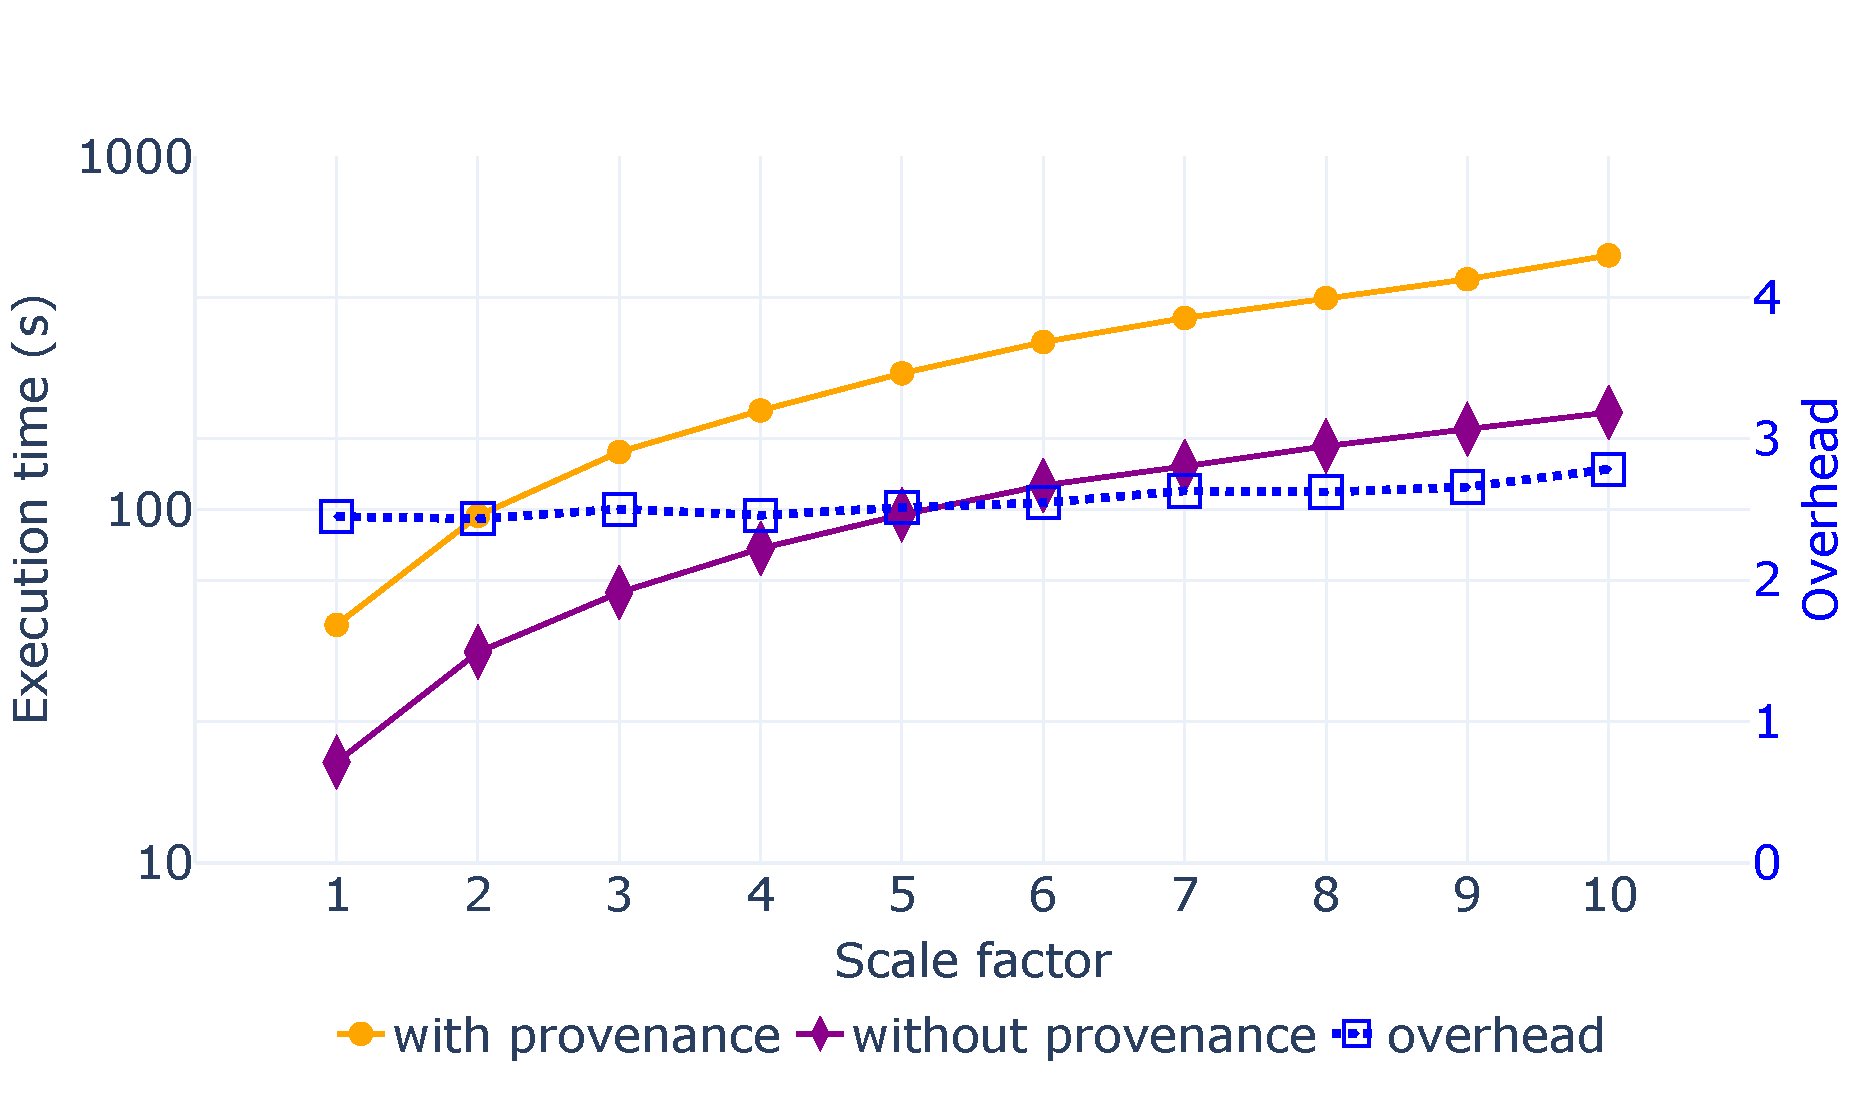
\includegraphics[width=\linewidth]{plots_pdf/overhead_qset.pdf}
		\caption{On the entire \qcust\ set}\label{fig:provsql_overhead_qset}
	\end{subfigure}
	\begin{subfigure}{\linewidth}
		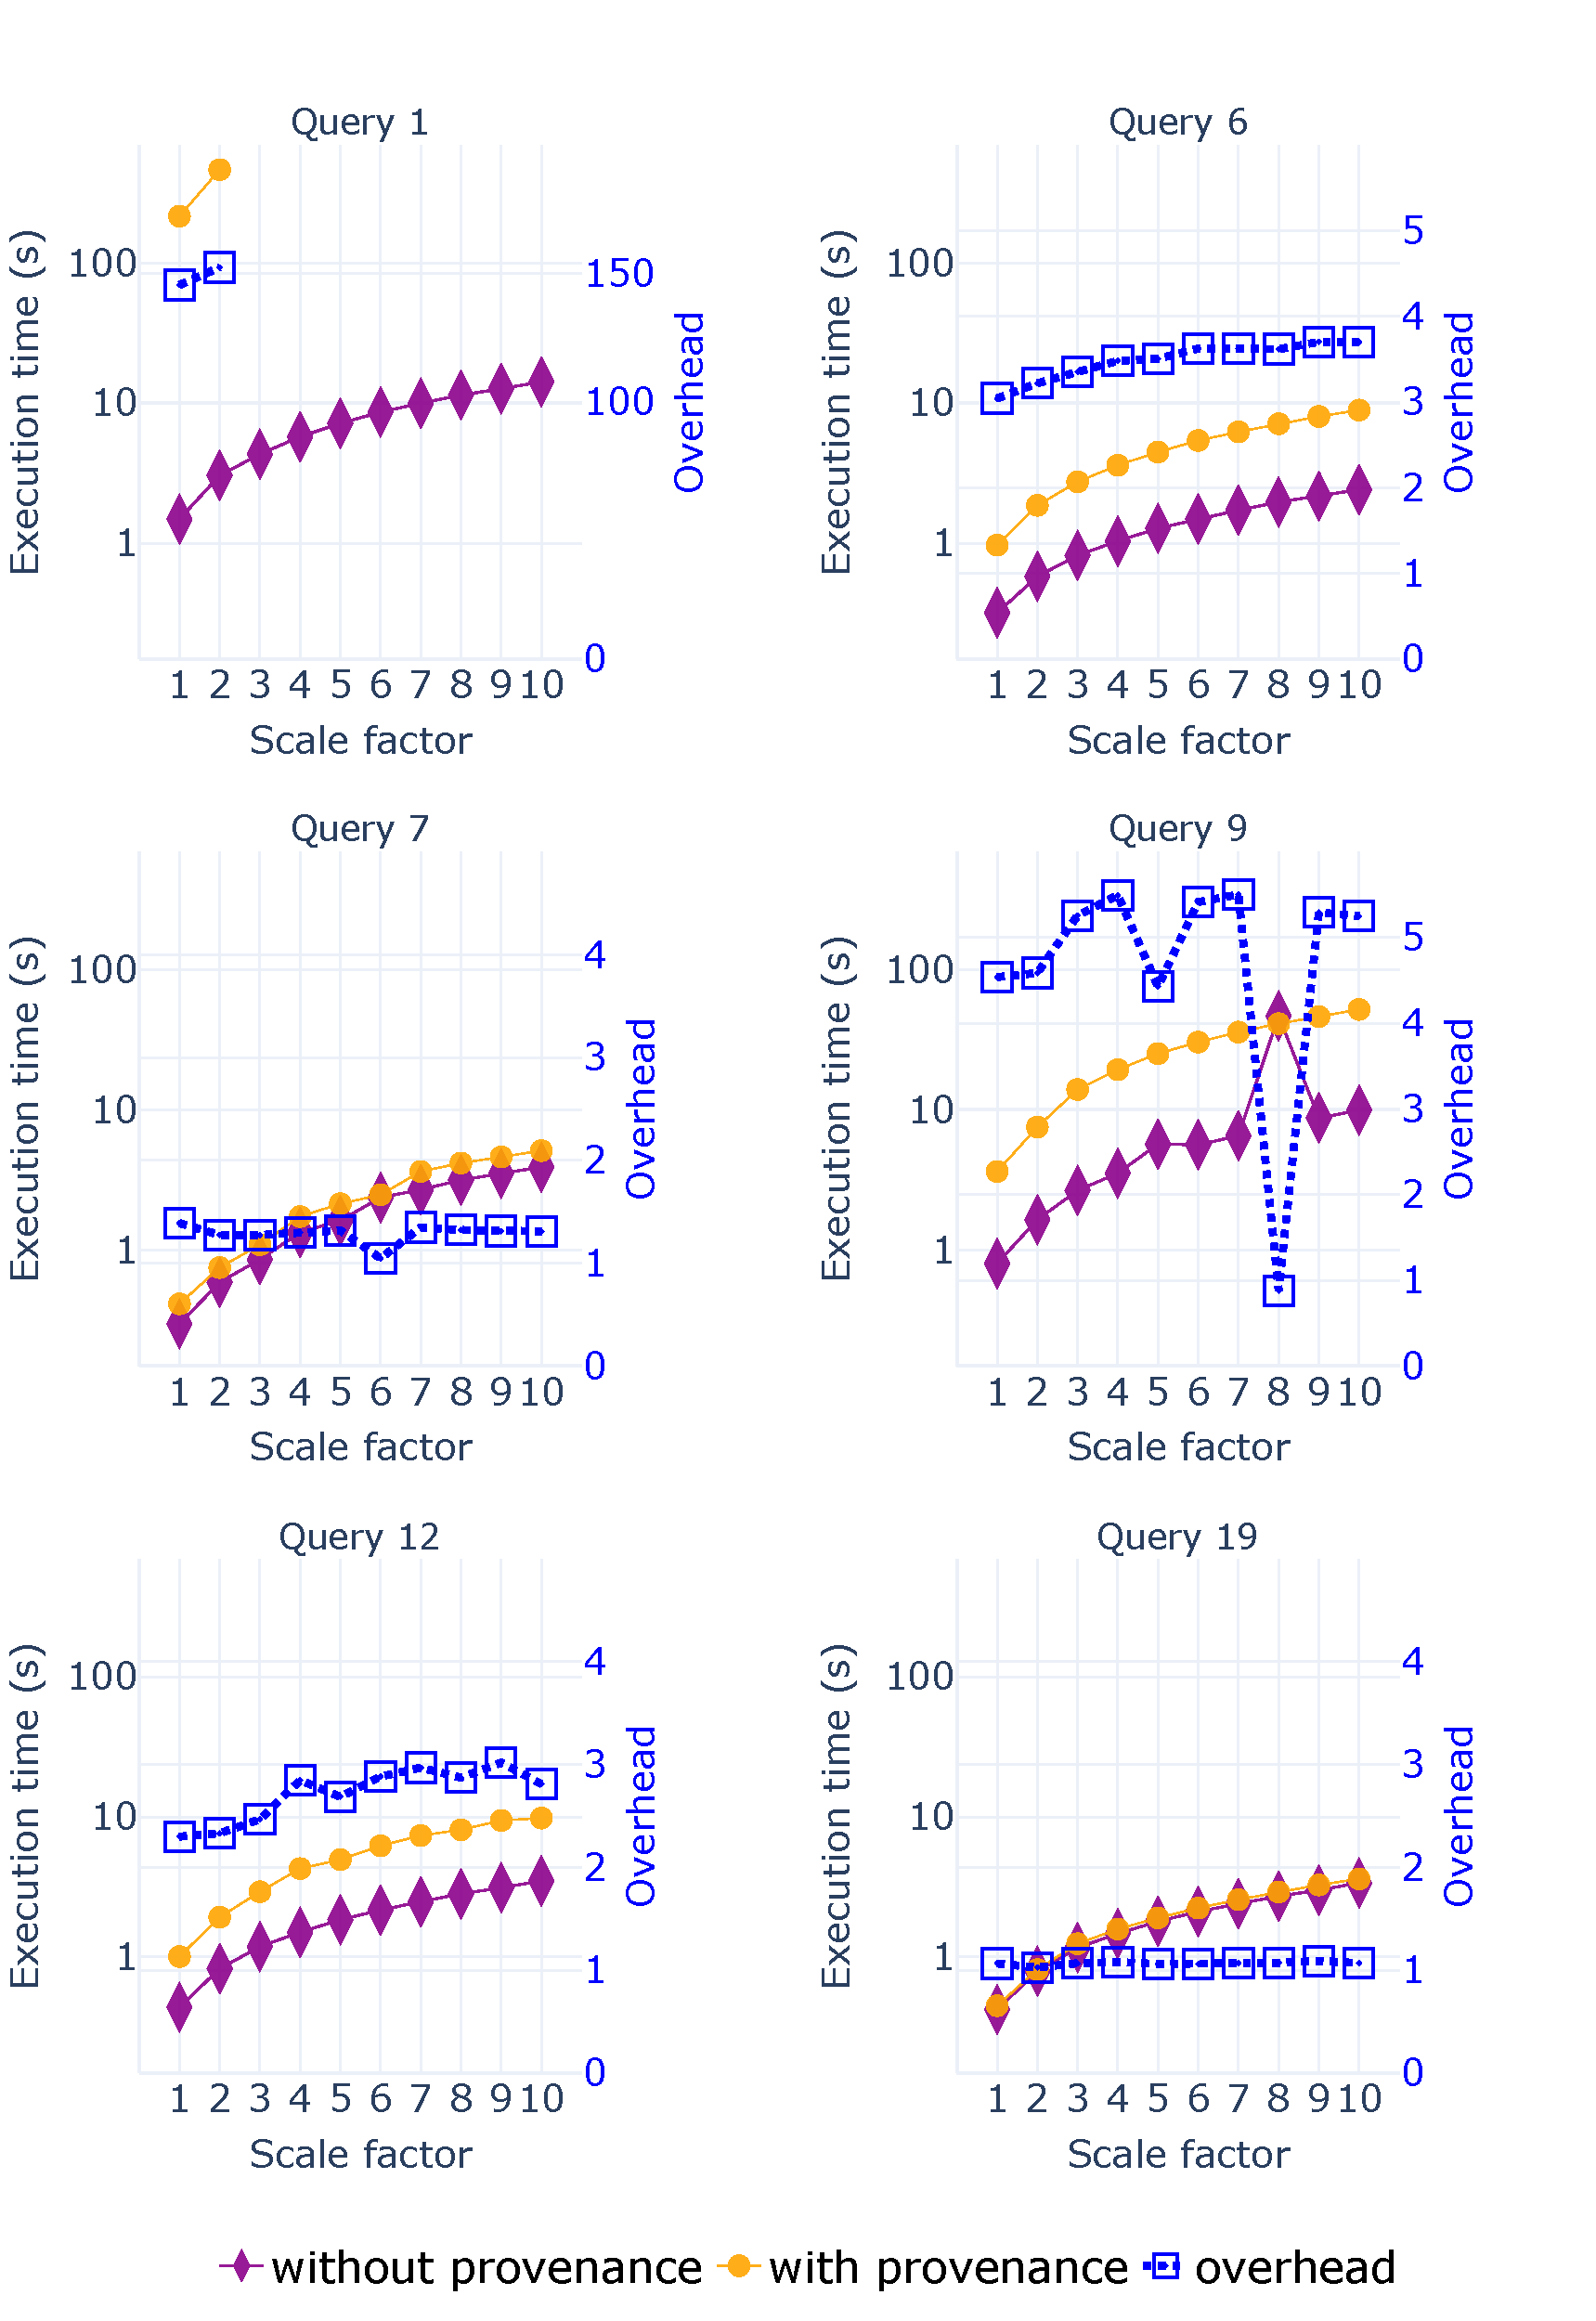
\includegraphics[width=\linewidth]{plots_pdf/overhead_tpch.pdf}
		\caption{On individual \qtpc\ queries}\label{fig:provsql_overhead_tpch}
	\end{subfigure}


	\caption{Scalability and provenance overhead: execution times (left $y$-axis, log-scale) and overhead (right $y$-axis, linear scale), at various scale factors ($x$-axis)}\label{fig:provsql_overhead}
\end{figure}



\paragraph*{Scalability and provenance overhead}
We compare the running time of queries over
PostgreSQL with the running time under ProvSQL, with provenance tracking
enabled, on TPC-H data of scale factors between 1 and 10. We are
especially interested in the overhead ratio, computed as
$\text{overhead}=\frac{t_{\text{provenance}}}{t_{\text{original}}}$.
We run the experiment on the entire \qcust query set, and on
individual queries from~\qtpc.
We show the results in Figure~\ref{fig:provsql_overhead}. Note that the blue curve corresponds
to the overhead, on the right (linear) y-axis of each plot, while the other two
curves use the left (logarithmic) y-axis.

On \qcust, Figure~\ref{fig:provsql_overhead_qset}
shows that the overhead is near-constant with the dataset size, indicating that provenance tracking scales at a similar rate as regular query execution.
This reflects the efficient implementation of provenance tracking by using provenance circuits in ProvSQL.

Results on \qtpc, Figure \ref{fig:provsql_overhead_tpch},
are of particular interest.
Query $19$ has a nearly constant overhead with little variation as the scale factor increases, characterizing efficient provenance tracking that scales independently of the database size.
For queries $7$ and $9$, we observe an anomalous \emph{decrease} in
overheads at certain scale factors due to PostgreSQL's query
optimizer adopting different execution plans when provenance tracking is
enabled, which happen to be better for that particular query. For
instance on query 9, the overhead at scale factor 8 completely
disappears. Indeed, in certain cases, provenance computation can
accidentally lead to performance improvement by guiding the PostgreSQL
optimizer to adopt a faster execution strategy. The size of the TPC-H
dataset incrementally increases with each scale factor and can cause
changes in join selectivity, indexing effectiveness and the optimizer's
cost estimates. For example, in queries $7$ and $9$ which have complex
joins, provenance tracking may force the optimizer to adopt a more
efficient join order. Except for these optimizer-driven fluctuations,
queries $7$ and $9$ have a constant overhead.
Queries $6$ and $12$ exhibit a high overhead that however remains under a
factor of~$4$, indicating scalability challenges in comparison to other
queries in this experiment. Query 6 does not involve any inner joins and
operates exclusively on the largest table in the dataset,
\texttt{lineitem}. The size of \texttt{lineitem} scales with the TPC-H
scale factor and also contains attributes with skewed, uniform, and
categorical distributions, making it a bottleneck for database optimizers
in situations where provenance tracking involves queries with a high
amount of filtering. For query $12$, the high overhead may be because of
the fact that it involves filtering conditions on aggregated tuples.
We note that ProvSQL cannot scale beyond scale factor $2$ for query~$1$ due
to memory limitations; at scale factor 1, the number of gates created in
the provenance circuit by ProvSQL for this query is
45.71M gates. For comparison, for query 7 it is 18.27k gates and
for query 9 it is 0.99M gates. Query 1 is a relatively broad query having a single filter on dates
filter along with $8$ aggregations on the
\texttt{lineitem} table, grouped on low-cardinality
columns such as \emph{l\_linestatus} and \emph{l\_returnflag}, thus limiting
scalability.
%and imposing unreasonable memory demands for higher scale factors.}


This experiment provides us with an important insight: while computing
provenance annotations generally adds overhead, this overhead is limited and even constant in most cases. It also indicates avenues for optimization of provenance computation, especially by reducing intermediate data structures.

\begin{figure}

	\begin{subfigure}{\linewidth}
		\centering
		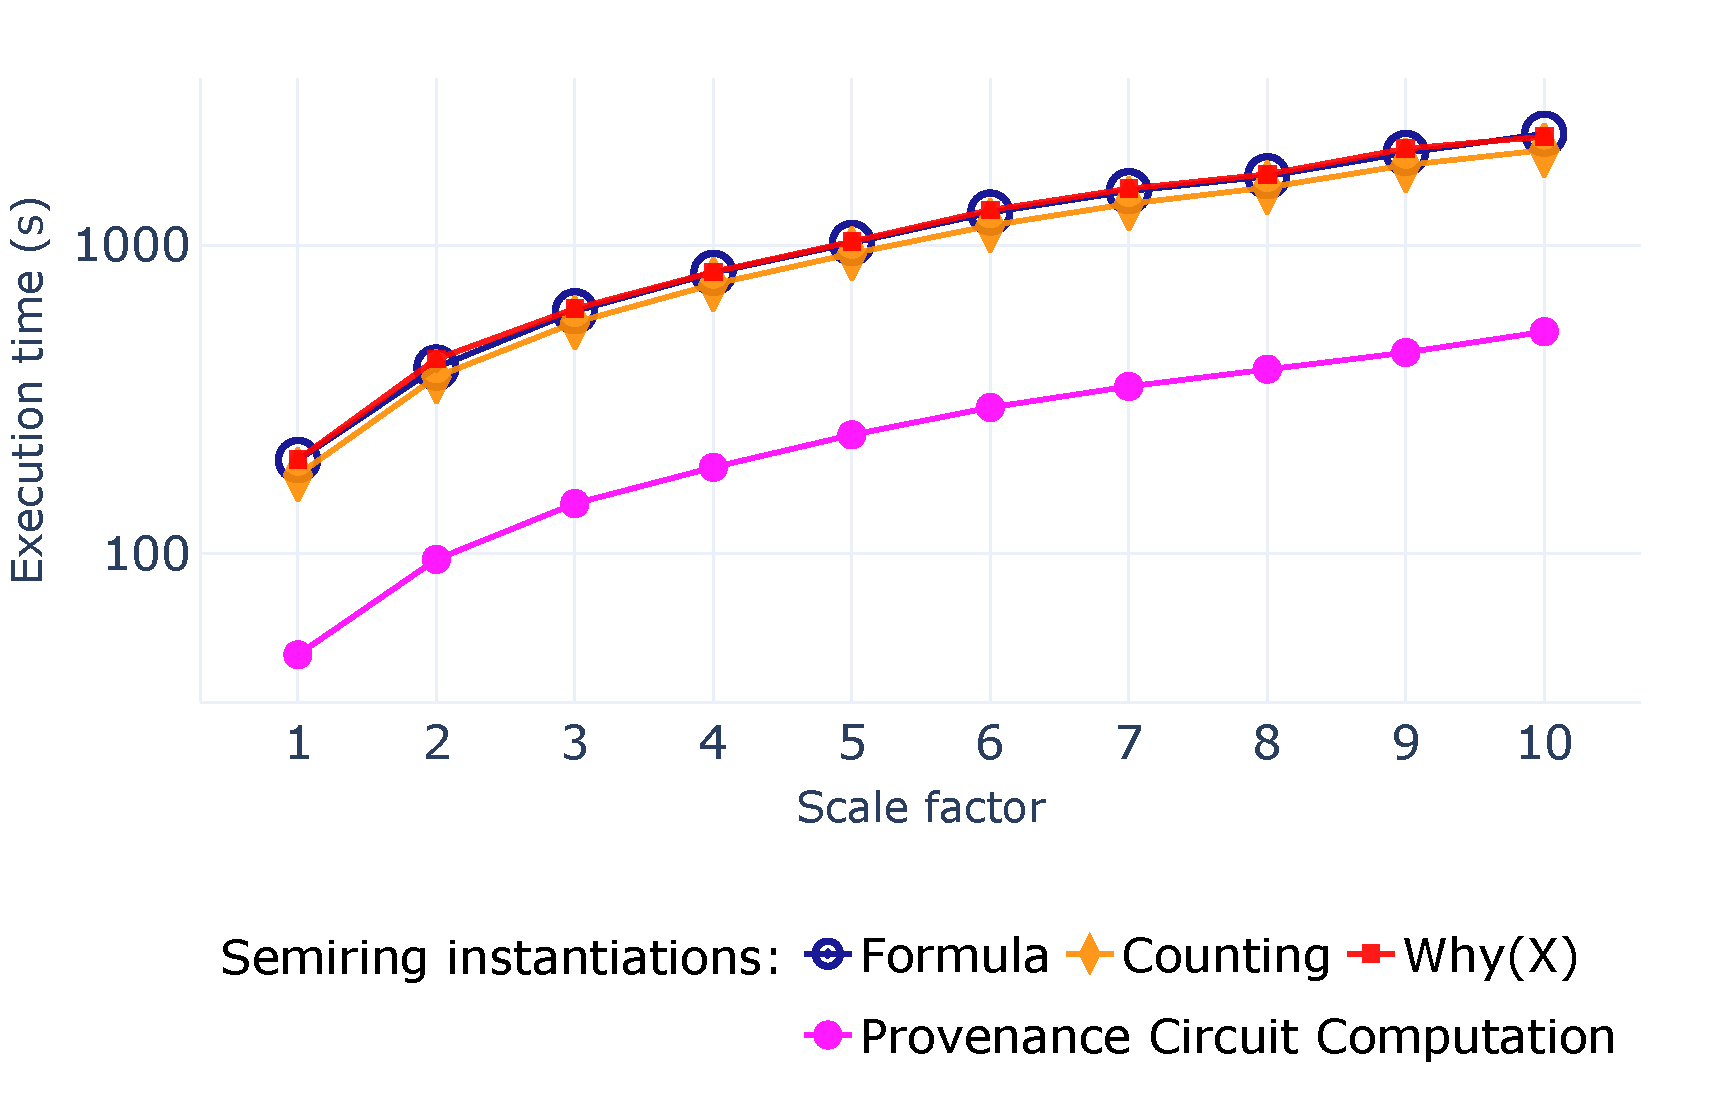
\includegraphics[width=0.8\linewidth]{plots_pdf/qset_semirings_provsql.pdf}
		\subcaption{On the entire \qcust\ set (log scale)}\label{fig:provsql_semirings_qset}
	\end{subfigure}
	\begin{subfigure}{\linewidth}
		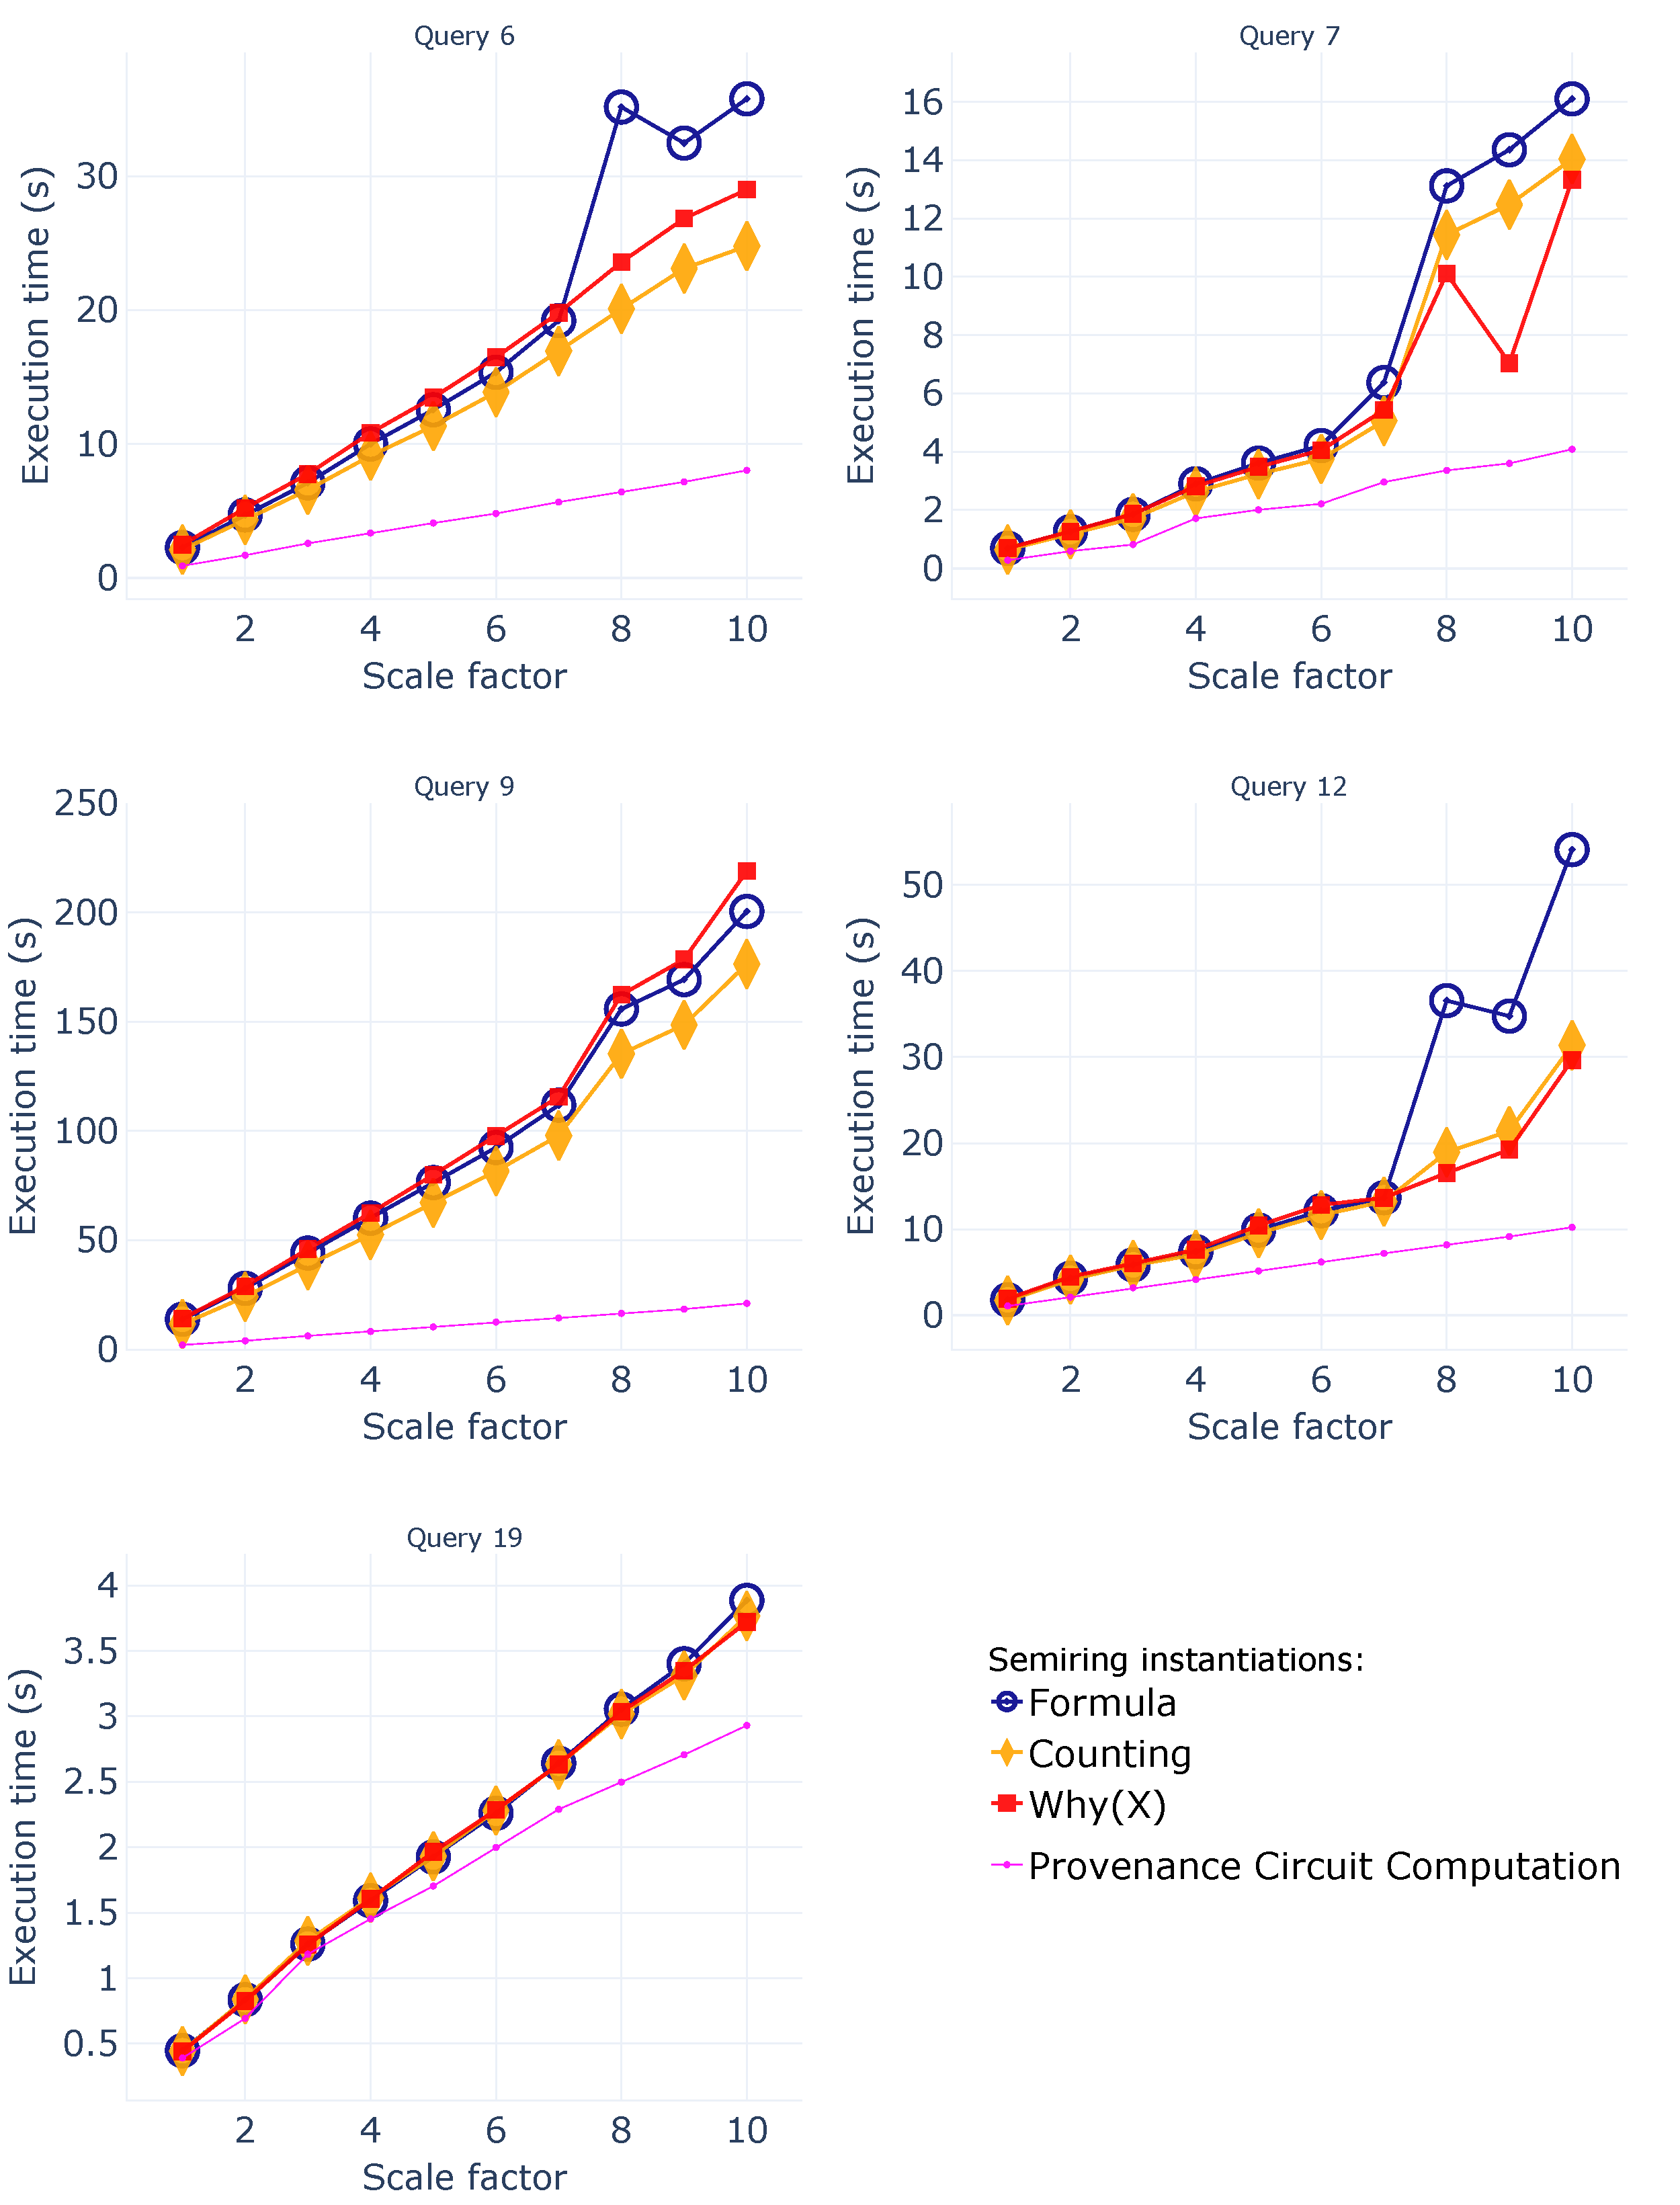
\includegraphics[width=\linewidth]{plots_pdf/semirings_tpch.pdf}
		\subcaption{On individual \qtpc\ queries  (linear scale)}\label{fig:provsql_semirings_tpch}
	\end{subfigure}


	\caption{Scalability of semiring instantiations in ProvSQL}\label{fig:provsql_semirings}
\end{figure}

\paragraph*{Semiring provenance evaluation}
We evaluate in Figure~\ref{fig:provsql_semirings} the overhead induced by
evaluating the resulting provenance circuits on different semirings
supported by ProvSQL (\emph{counting}, \emph{why-provenance}, as well as a
pseudo-semiring that just serializes in a \emph{formula}-based
representation the provenance circuit), on the TPC-H database across
scale factors 1 to 10. On the queries in \qcust\
(Figure~\ref{fig:provsql_semirings_qset}) we observe linear
trends, with the semiring instantiations across TPC-H scale factors 1 to
10. All three of the semirings introduce
virtually the same overhead to provenance computation.
The overheads observed are constant with the database size, as
none of the queries in \qcust\ have aggregates. This increased efficiency compared to aggregate provenance is due to the fact provenance computation for aggregates involves poly-sized overheads caused by
the $K-$semimodule operations.

Figure~\ref{fig:provsql_semirings_tpch} shows the overheads incurred for
individual \qtpc{} queries. We omit query 1 from \qtpc\ in this
experiment, as we just saw ProvSQL does not scale for  query 1 even when
we are only computing the provenance circuit. Except for query 9 the execution times for
the semiring instantiations indicate minimal poly-sized overheads over circuit computation times.

\paragraph*{Comparing scalability and performance queries 7 and 9 of \qtpc}
We detail the functioning of queries 7 and 9 for different implementation of ProvSQL, as we consider they are representative to some possible optimizations. Figure~\ref{fig:provsql_versions} (left) shows the scalability of three different versions of ProvSQL, implementing provenance circuits differently. Due to compatibility issues with the older implementations of circuits in ProvSQL we had to to run this experiment on PostgreSQL 14.
The current version of ProvSQL (\emph{provsql\_mmap}), which uses memory-mapped files, has the fastest running times of all three. Moreover, the running time scales linearly. The shared-memory version of ProvSQL (\emph{provsql\_shm}), in which circuits are kept in the PostgreSQL shared memory, does not scale beyond TPC-H
scale factor 4. The shared-memory implementation is also slower than the memory-mapped implementation; this is due to the impossibility to parallelize the PL/pgSQL functions that use LOCK on \emph{aggregate values}.
Although the in-database implementation of ProvSQL (\emph{provsql\_indb}), where provenance circuits are stored as PostgreSQL tables, scales linearly, it has the slowest running times.

Figure~\ref{fig:provsql_versions} (right) shows the number of gates created by ProvSQL in the provenance circuit on evaluation of the query. We can see that the number of gates created at each scale factor is significantly higher when executing query 9 of \qtpc\ than query 7. This is because, even though queries 7 and 9
 of \qtpc\ have the same number of joins and aggregations, query 9 is more selective than query 7. This also explains why the execution time for query 9 is significantly higher than query 7, and suggests that reducing the number of gates created in the provenance circuit is a good direction for future optimizations.

\begin{figure}
    \centering
        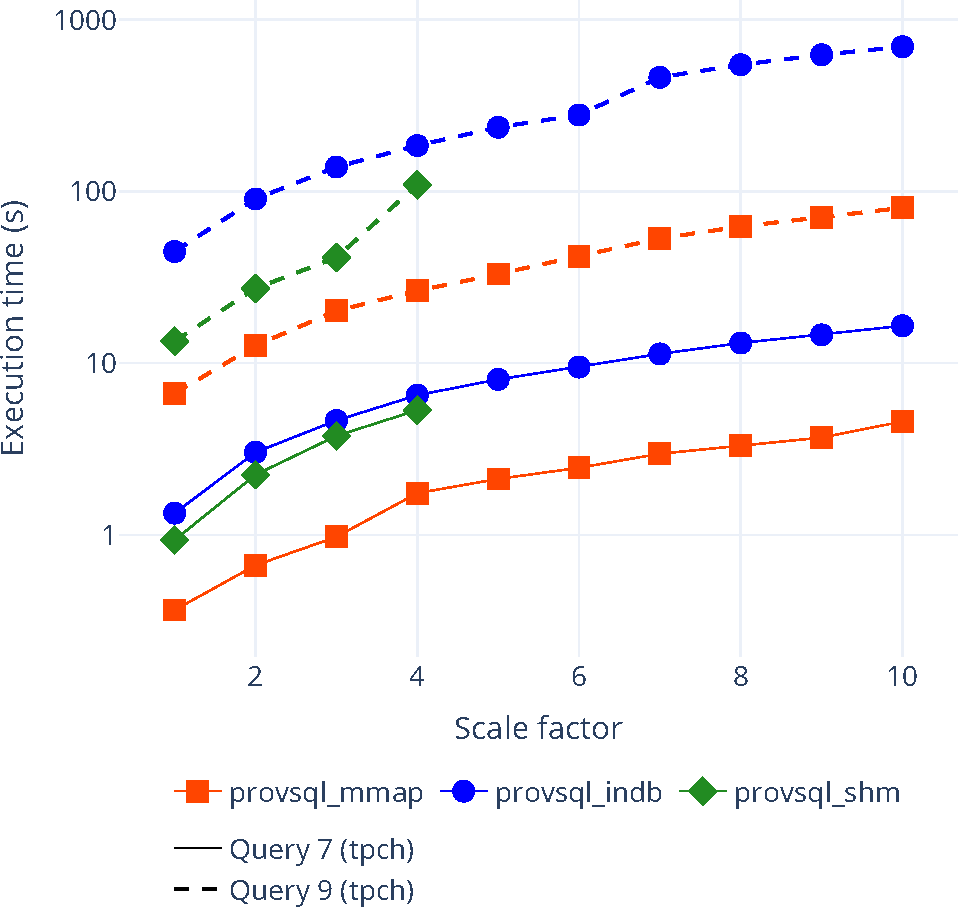
\includegraphics[width=0.48\linewidth]{plots_pdf/provsql_versions.pdf}
        \hfill
        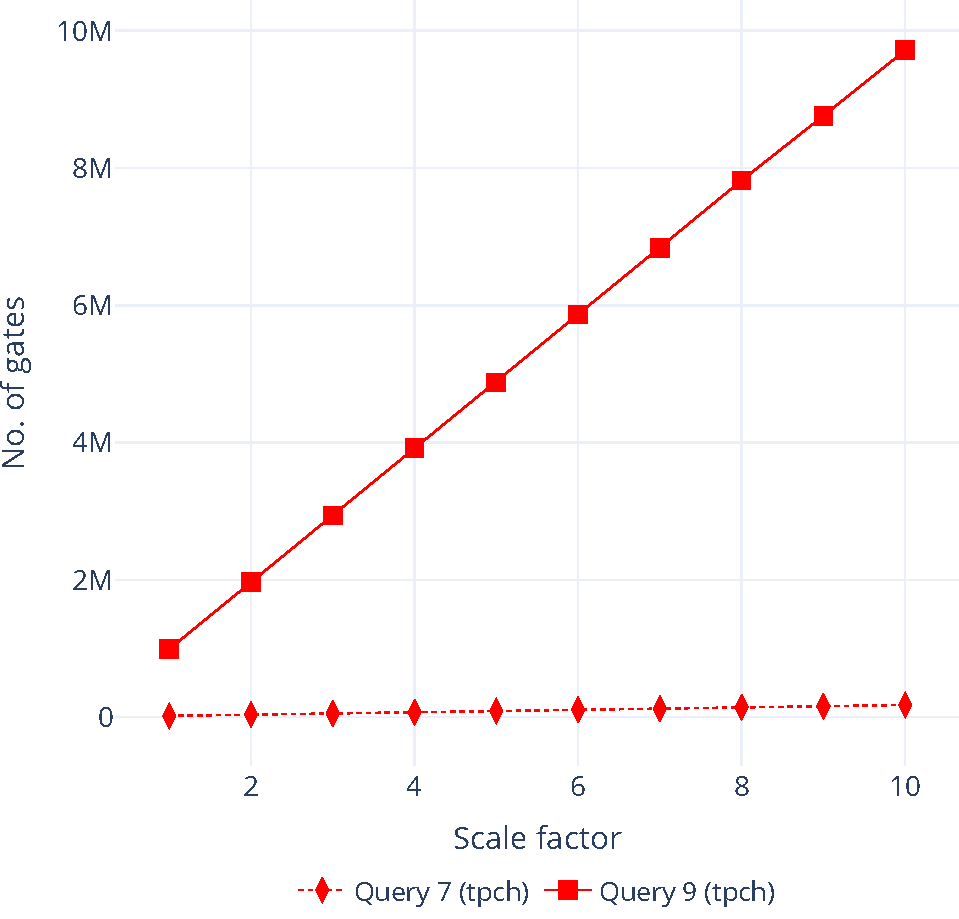
\includegraphics[width=0.48\linewidth]{plots_pdf/circuit_size_difference.pdf}
        \caption{Detailed analysis of ProvSQL on queries 7
          and 9 from \qtpc\ for different TPC-H scale factors. Left: scalability and performance of different ProvSQL
          versions (log scale). Right: number of extra gates of the provenance circuit.}
        \label{fig:provsql_versions}
\end{figure}

\begin{figure}

	\begin{subfigure}{0.4\linewidth}
		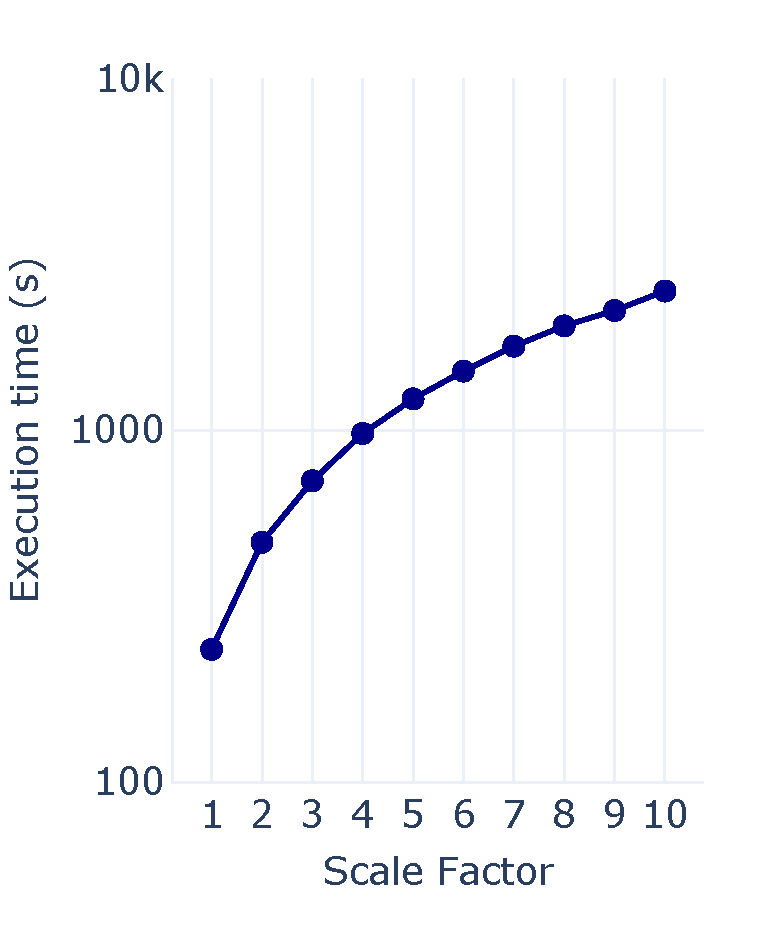
\includegraphics[width=1.2\linewidth]{plots_pdf/provsql_probab_qset.pdf}
		\subcaption{On the entire \qprob\ set (log scale)}\label{fig:provsql_prob_qset}
	\end{subfigure}%
	\hfill
	\begin{subfigure}{0.5\linewidth}
		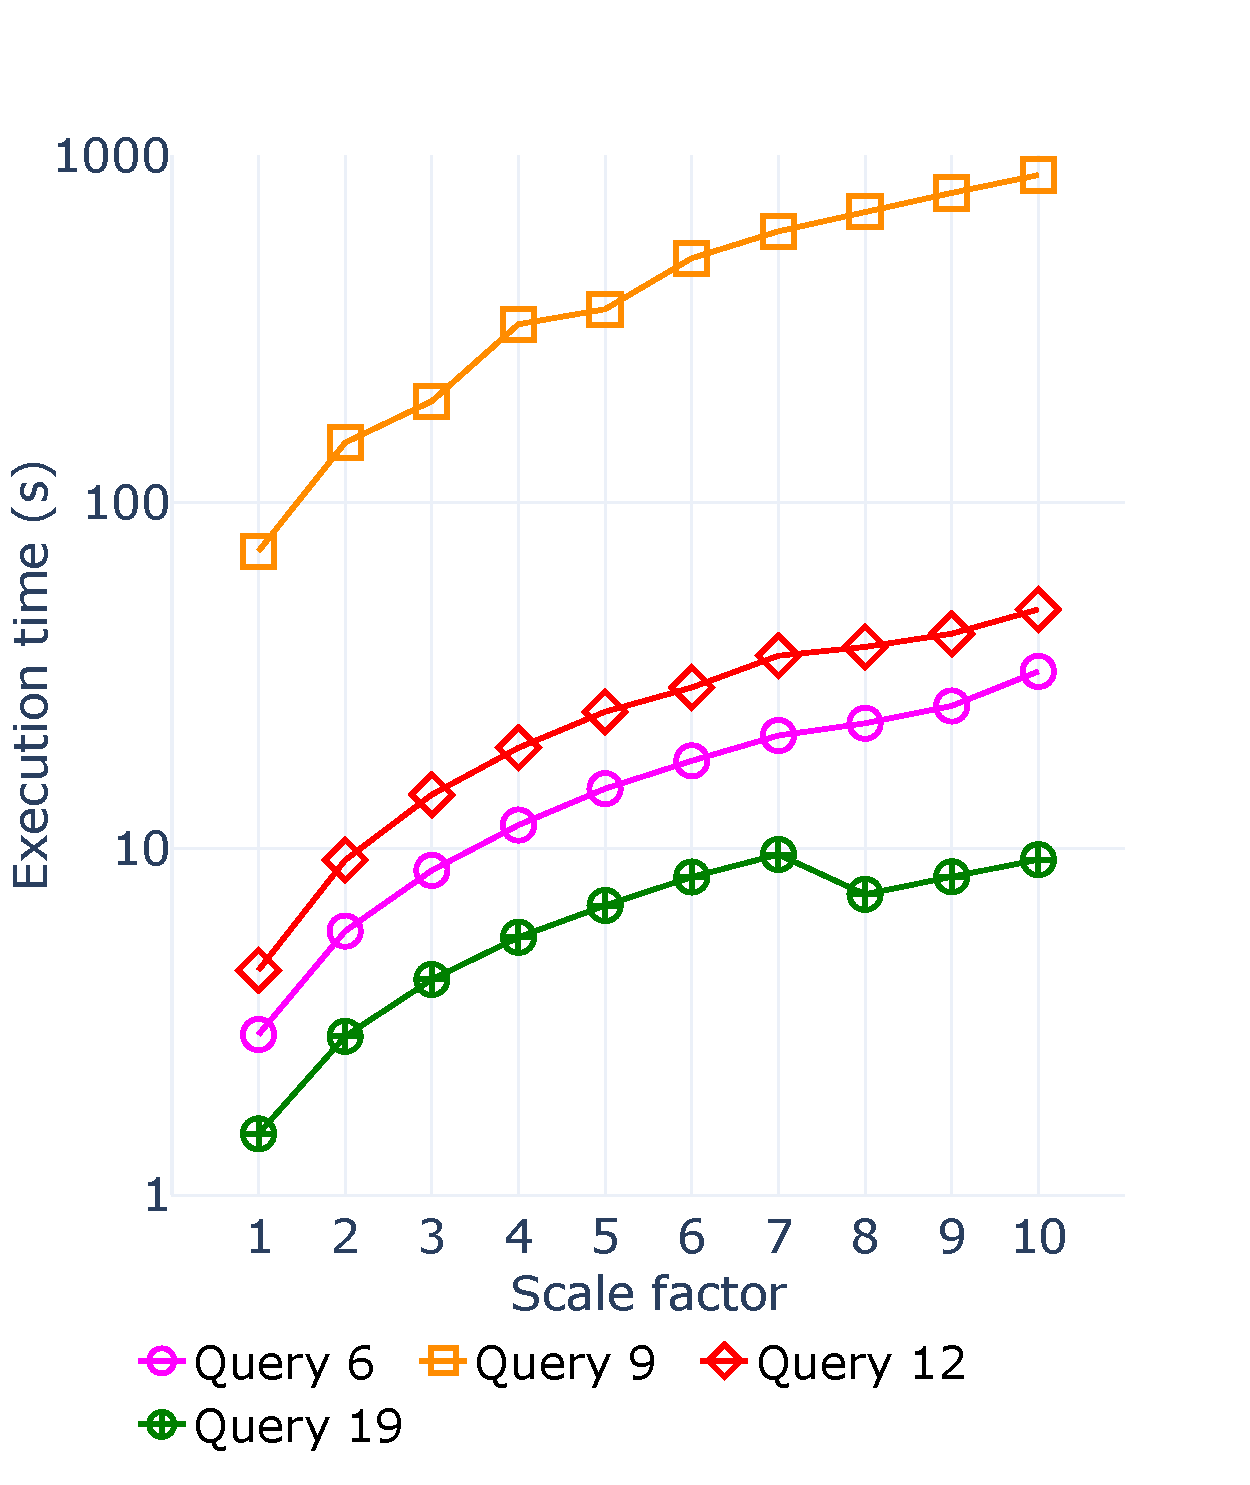
\includegraphics[width=\linewidth]{plots_pdf/probabilities_tpch_provsql.pdf}
		\subcaption{On individual \qtpc\ queries (log scale)}\label{fig:provsql_prob_tpch}
	\end{subfigure}

	\caption{Scalability of probability computation in ProvSQL}\label{fig:provsql_prob}
\end{figure}
\paragraph*{Probability evaluation}
Query 9 in \qcust\ has 8 joins and ProvSQL goes out of memory while
computing probabilities for it (more precisely, the knowledge compiler d4
called by ProvSQL runs out of memory).
We omit query 9 from \qcust\ and denote this new query set as \qprob.
Figure{~\ref{fig:provsql_prob_qset}} shows that ProvSQL scales linearly with the dataset size, when computing probabilities on query set \qprob.

Figure~\ref{fig:provsql_prob_tpch} shows generally linear scalability trends across queries 6, 9, 12, 19 from \qtpc. The exception is query 19: some optimizer driven fluctuations generate counter-intuitive performance \emph{gains} between scale factors 7 and 9. For queries 1 and 7 (not shown here) ProvSQL goes out of memory when computing probabilities, for the same reasons as outlined in the provenance overhead experiment.




\subsection{GProM vs ProvSQL for Provenance}
We now compare the performance of ProvSQL to that of GProM for computing
the provenance of query results.

\begin{figure}

		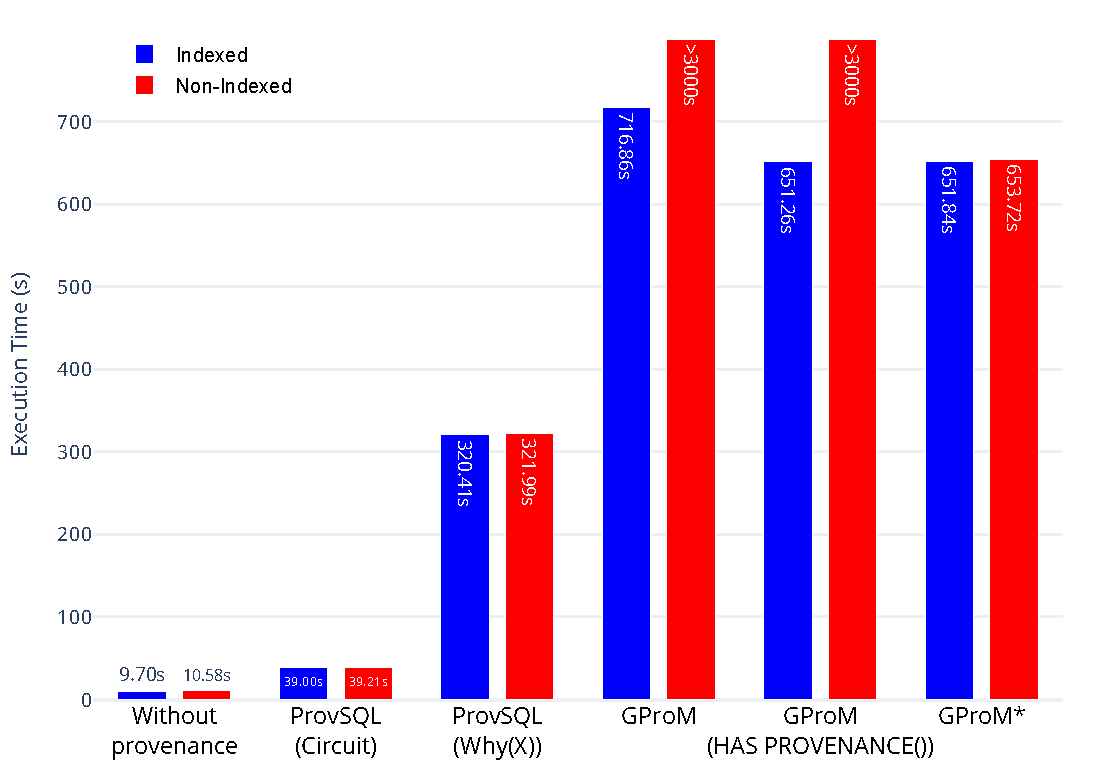
\includegraphics[width=\linewidth]{plots_pdf/indexing.pdf}
		\caption{GProM vs ProvSQL on 1 GB TPC-H dataset (with and without indexing) for \qgprom\ }\label{fig:index}

\end{figure}

We compare the execution times of provenance tracking for GProM and ProvSQL
on \qgprom, consisting of all queries in \qcust\ that GProM supports (see
Table~\ref{tab:sys_comp}) in Figure~\ref{fig:index}.
By using GProM's \mintinline{sql}{HAS PROVENANCE()} construct on the primary keys of the
tables used in a query, GProM can compute provenance expressions that closely resemble
the form of why-provenance defined in semiring-based provenance models.
However, in \mbox{TPC-H}, the primary keys are defined separately for each individual table. They cannot be used as provenance annotations because
provenance annotations, by construction, should be globally unique across the entire database.
Since GProM does not use global identifiers, we created composite primary keys for each table in the
TPC-H dataset by prefixing the table name to the primary keys and call
\mintinline{sqL}{HAS PROVENANCE()} on the composite primary keys.

We first consider the impact of indexing on the performance of these
systems.
In TPC-H, no indices (primary keys, unique constraints, etc) are defined
by default, and it is usually advised not to use indexes to compare the
performance of classical relational database systems on this dataset. In
small-scale datasets, the benefit of indexing on TPC-H queries is
actually negligible. We can observe this in Figure~\ref{fig:index} (scale
factor~1) for PostgreSQL runtime and
provenance computation using ProvSQL. However for GProM, indexing
dramatically reduces the execution time. Post-indexing, GProM yields
better results when using \mintinline{sql}{HAS PROVENANCE()}.
The bars labeled GProM$^*$ shows normalized execution
  times of GProM (with \mintinline{sql}{HAS PROVENANCE()}) rewritings, evaluated
  directly within PostgreSQL, without relying on query evaluation in
  GProM. This allows direct comparison of the query rewriting approaches
  between GproM and ProvSQL. The reported times are the total execution time of both query
  rewriting and query evaluation.


\begin{figure}
		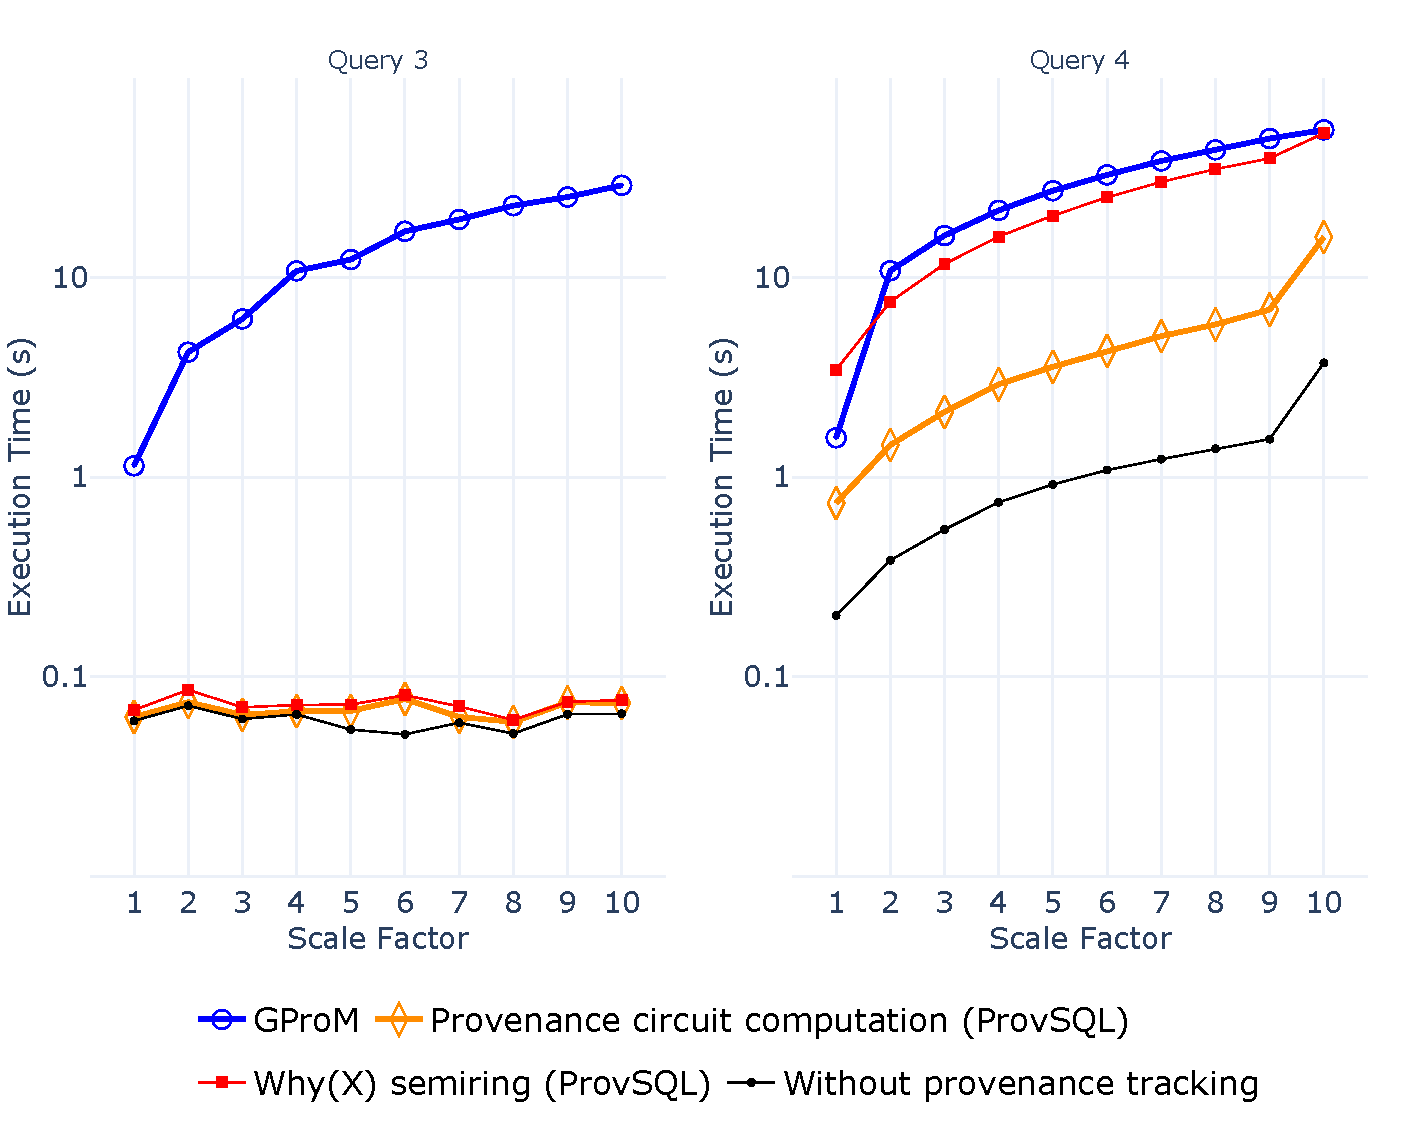
\includegraphics[width=\linewidth]{plots_pdf/gprom_tpch.pdf}
	    \caption{Scalability of GProM vs ProvSQL on query 3 and~4 from \qtpce\ (log scale)}\label{fig:gprom_tpch}
\end{figure}


In Figure~\ref{fig:gprom_tpch} we compare the scalability of provenance tracking in GProM with ProvSQL on queries 3 and 4 from \qtpce\ .
These queries are simple queries without aggregation. For query~3
the number of output tuples is limited to 20 and provenance tracking is
highly efficient across scale factors for ProvSQL. The semiring instantiations incur negligible overhead over baseline execution times
and circuit computation times. Even though GProM underperforms relatively to ProvSQL, it scales linearly.
For query 4 there are no constraints on the number of output tuples. Both ProvSQL and GProM scale linearly. The semiring instantiations in ProvSQL
incur constant overhead throughtout the scale factors. For query 4
GProM's execution times are slightly higher (except at scale factor~1).
% We compare the scalability of provenance tracking in GProM vs ProvSQL
% on \qgprom, consisting of all queries in \qcust\ that GProM supports (see
% Table~\ref{tab:sys_comp}) in Figure~\ref{fig:gprom_qset}. We outline some scalability issues with GProM.
% For scale factors 7, 8 and 9  GProM takes more than $25\,000$ seconds whereas for scale factor 10 it runs out of memory and crashes even before the timeout threshold. ProvSQL exhibits a significant overhead when it comes to provenance computation on the why-provenance semiring, but even then it scales linearly with TPC-H scale factors, unlike GProM which seems to show exponential growth in execution times.

% We zoom in on this experiment for query 3 from \qtpce\, as GProM does not
% support any of the original TPC-H queries. In Figure~\ref{fig:gprom_tpch}
% (note the y-axis is cut in two parts for readability of both
% sets of plots), we see that GProM exhibits
% exponentially increasing execution times, indicating poor scalability. At scale factor 10, GProM crashes and goes out of memory while running query 3.

% GProM's provenance representation -- discussed in detail in the supplementary material -- may be the main reason for this scalability
% issue. The size of provenance expressions (represented by extra
% attributes) can grow significantly with the number of joins. While ProvSQL benefits from efficient provenance representations, GProM's explicit tuple-level provenance annotations, by means of appending duplicates of entire tuples with renamed schema features, results in poor scalability. Although ProvSQL shows a noticeable overhead when evaluating semirings on top of the provenance circuits, it still outperforms GProM by a large margin. Moreover, Figure~\ref{fig:gprom_tpch} again shows that ProvSQL, at certain scale factors, may benefit from optimizer-driven performance improvements, as previously discussed.

\begin{figure}
	\begin{subfigure}{\linewidth}
		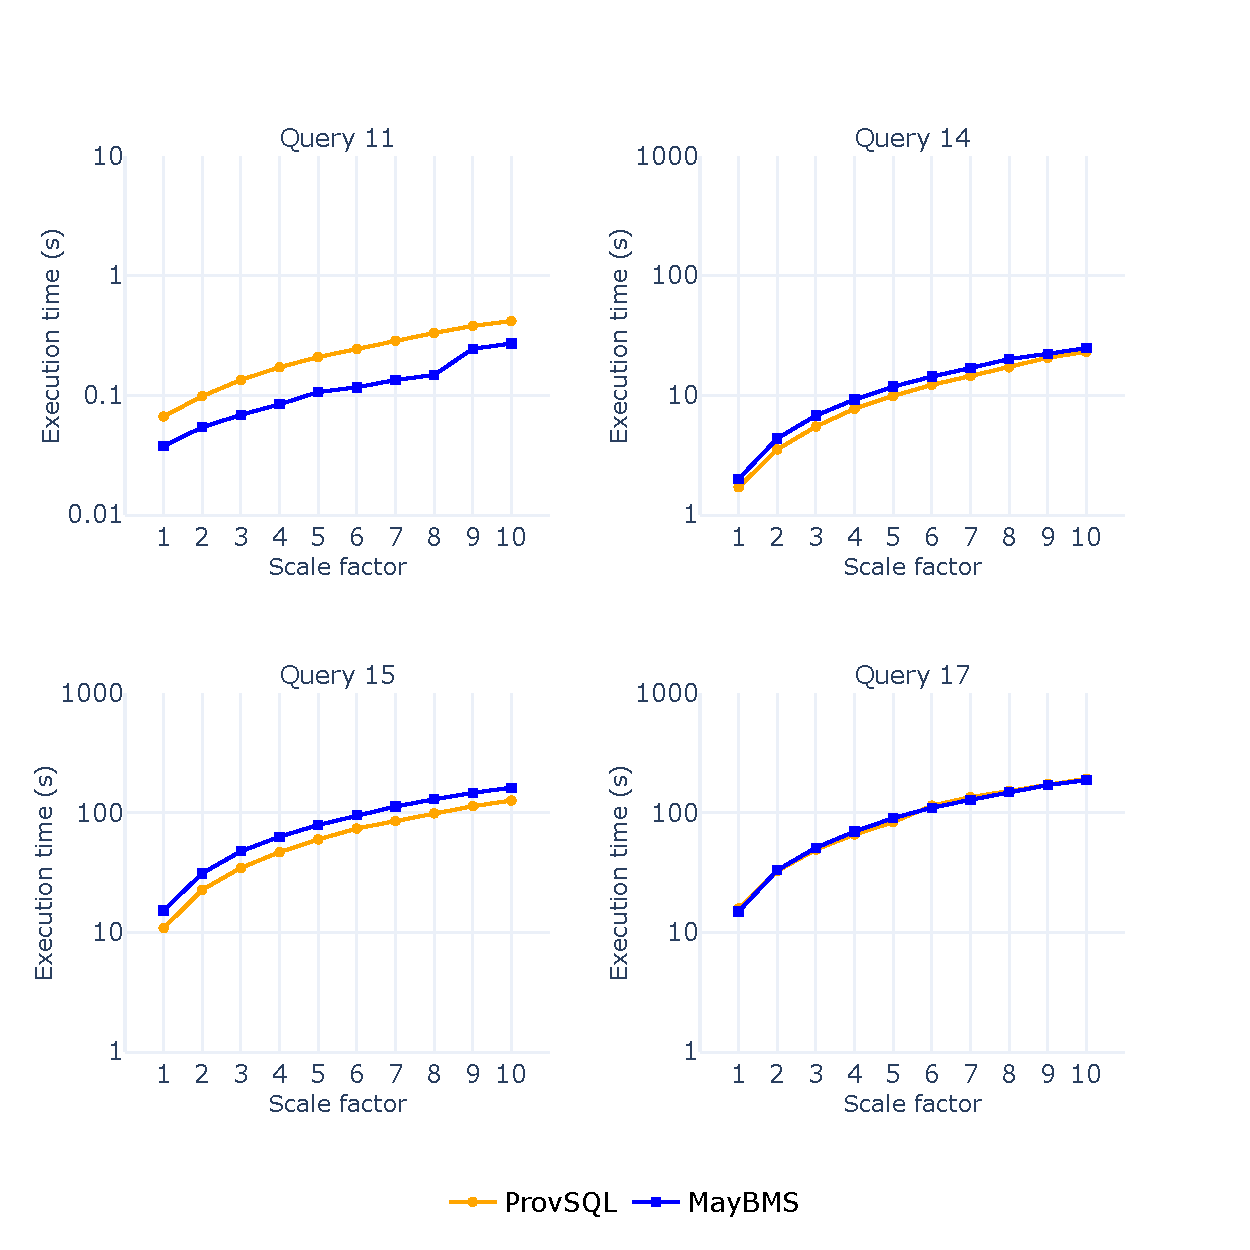
\includegraphics[width=\linewidth]{plots_pdf/unsafe.pdf}
		\subcaption{On queries 11, 14, 15 and 17 from $\mathcal{Q}^{MayBMS}$ (log scale)}\label{fig:unsafe}
	\end{subfigure}
  \vspace{-1.2em}

	\begin{subfigure}{\linewidth}
		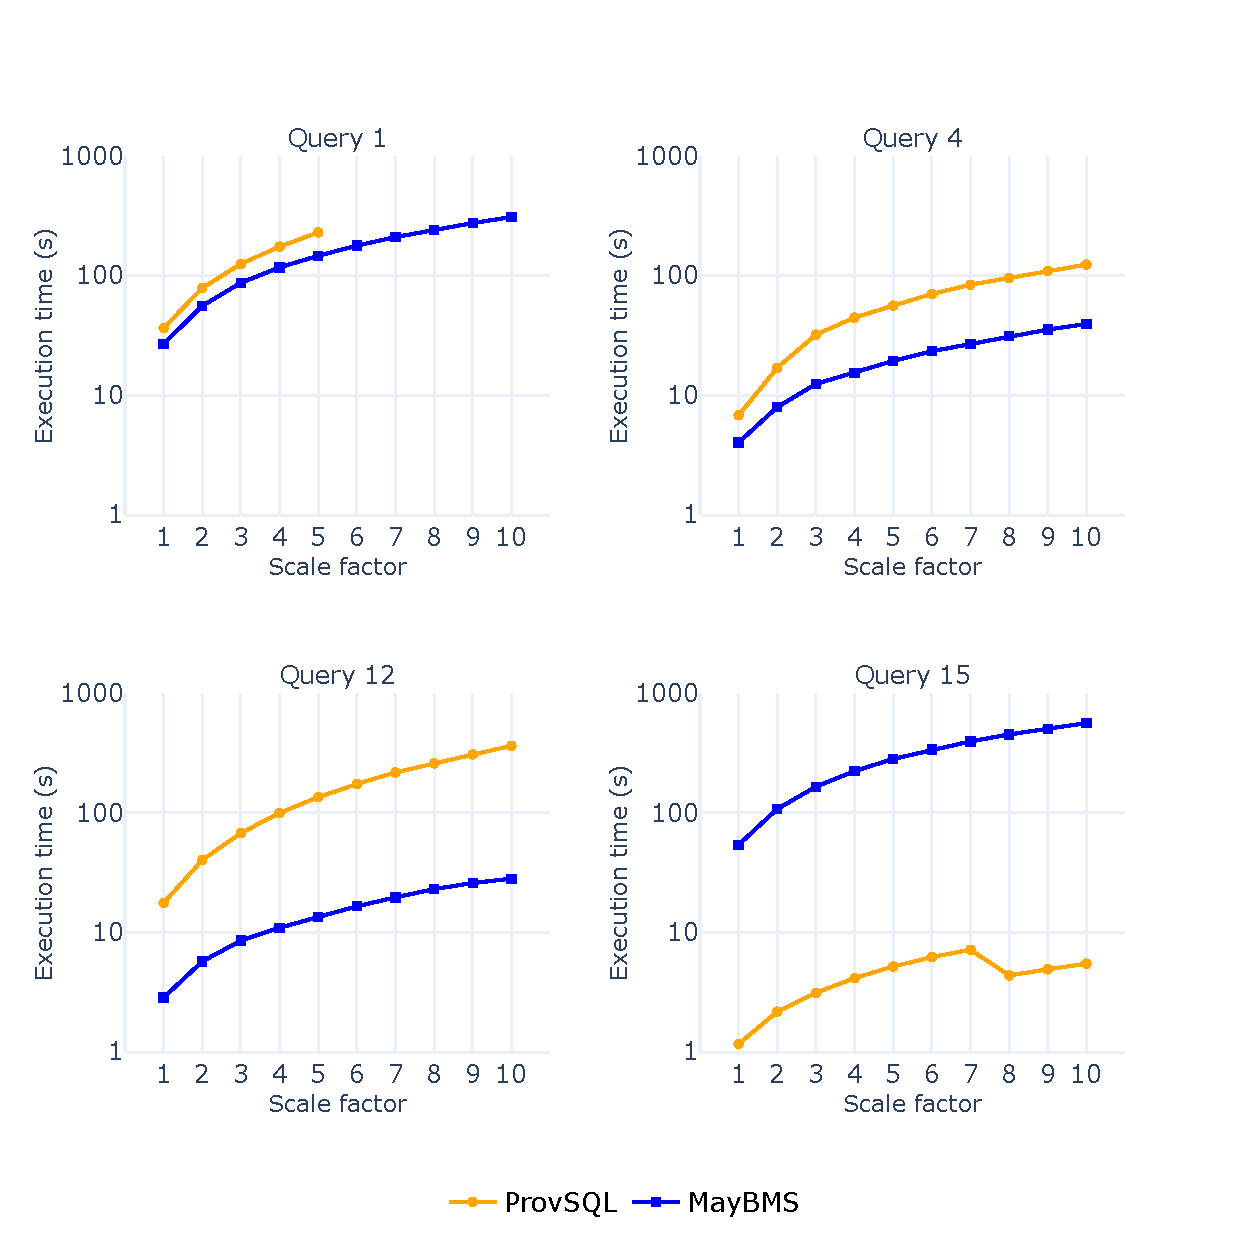
\includegraphics[width=\linewidth]{plots_pdf/maybms_provsql_tpch.pdf}
		\subcaption{On queries 1, 4, 12 and 15 from \qtpce\ (log scale)}\label{fig:safe}
	\end{subfigure}

	\caption{Scalability of MayBMS vs ProvSQL}
\end{figure}

\subsection{MayBMS vs ProvSQL for Probability}
We compare the scalability of ProvSQL and MayBMS when it comes to probability computation on uncertain tuple-independent databases, excluding queries involving set operations and aggregations, that MayBMS does not support (see Table~\ref{tab:sys_comp}).
The queries used in this experiment were rewritten
for MayBMS to adhere to the syntax constraints of this system.
%, in
%particular using
%\mintinline{sql}{conf()} and \mintinline{sql}{tconf()} were appropriate.

MayBMS implements efficient query plans for \emph{safe
	queries}~\cite{dalvi2013dichotomy}, something ProvSQL does not.
We first select 4 queries that are not safe (11, 14, 15 and 17), from our set of
custom queries for which MayBMS can compute probabilities; this query set
is denoted as \qmay.
Figure~\ref{fig:unsafe} shows that both ProvSQL and MayBMS perform similarly on all 4 queries, exhibiting linear growth with TPC-H scale factors. ProvSQL performs slightly better on queries 14 and 15; ProvSQL and MayBMS have nearly the same execution times for query 17.

We also compared ProvSQL with MayBMS by carrying out probability
computations on the modified TPC-H queries, which were used to benchmark
MayBMS. These are the largest subqueries from the original TPC-H queries
$1$, $4$, $12$, and $15$ but without aggregations and inequality joins.
Figure~\ref{fig:safe} shows how MayBMS and ProvSQL scales against the
TPC-H scale factors. For query 1, ProvSQL goes out of memory beyond scale
factor~5. Both systems scale linearly with dataset size, but MayBMS
performs noticeably better than ProvSQL on queries 1, 4 and 12. This
difference in their performance is mainly because MayBMS
and ProvSQL have different approaches when it comes to probability
evaluation. In this experiment all queries are safe and MayBMS employs
safe query plans which often results in efficient probability evaluation.
ProvSQL does not implement the safe query approach. It is designed to be
a generic system that allows provenance tracking and also offers
probability computation by means of Boolean provenance circuits. When
provenance circuits exceed manageable limits it resorts to knowledge
compilers, which may be unable to exploit the structure of the
provenance formula. In some queries, however, such as query 15, this
mechanism allows ProvSQL to compute probabilities faster than
MayBMS.

\begin{toappendix}
	\section{DSQGEN query templates for queries in \qcust}
	\begin{minted}[autogobble,fontsize=\small]{postgresql}
  -- Query 1:
  define QUANT=RANDOM(1,50,uniform);
  define MODE=TEXT({"REG AIR",1},{"AIR",1},{"RAIL",1},
  {"SHIP",1},{"TRUCK",1},{"MAIL",1},{"FOB",1});
  define DISC=RANDOM(0,10,uniform);
  SELECT l_orderkey, l_partkey, l_suppkey,
  l_linenumber, l_linestatus
  FROM lineitem
  WHERE l_shipmode = '[MODE]'
  AND l_quantity > [QUANT]
  OR l_discount >= cast([DISC] as float)/100.0;

  -- Query 2:
  define NATION=RANDOM(0,24,uniform);
  define PRICE=RANDOM(10000,100000,uniform);
  SELECT DISTINCT o.o_orderdate, o.o_custkey
  FROM orders o, customer c
  WHERE o.o_custkey = c.c_custkey
  AND o.o_totalprice > [PRICE]
  AND c.c_nationkey = [NATION]
  AND o.o_orderstatus IN ('P','F');

  -- Query 3:
  define REGION=RANDOM(0,4,uniform);
  define COST=RANDOM(1,1000,uniform);
  SELECT p.p_name, p.p_mfgr, p.p_partkey, p.p_retailprice
  FROM part p
  INNER JOIN partsupp ps ON p.p_partkey = ps.ps_partkey
  INNER JOIN supplier s  ON ps.ps_suppkey = s.s_suppkey
  INNER JOIN nation n    ON s.s_nationkey = n.n_nationkey
  INNER JOIN region r    ON n.n_regionkey = r.r_regionkey
  WHERE r.r_regionkey = [REGION]
  AND ps.ps_supplycost < [COST];

  -- Query 4:
  define PRICE=RANDOM(10000,100000,uniform);
  SELECT DISTINCT c.c_name, c.c_nationkey
  FROM customer c, orders o
  WHERE c.c_custkey = o.o_custkey
  AND o.o_totalprice > [PRICE]
  GROUP BY c.c_nationkey,c.c_name;

  -- Query 5:
  define COST=RANDOM(100,1000,uniform);
  define AVAIL=RANDOM(1,8888,uniform);
  SELECT s.s_name, s.s_address, s.s_phone
  FROM supplier s INNER JOIN partsupp ps
  ON s.s_suppkey = ps.ps_suppkey
  WHERE ps.ps_supplycost > [COST]
  OR (ps.ps_availqty > [AVAIL] AND
  ps.ps_supplycost > cast([COST] as float)/2);

  -- Query 6:
  define A=TEXT({"STANDARD",1},{"SMALL",1},{"MEDIUM",1},
  {"LARGE",1},{"ECONOMY",1},{"PROMO",1});
  define B=TEXT({"ANODIZED",1},{"BURNISHED",1},{"PLATED",1},
  {"POLISHED",1},{"BRUSHED",1});
  define C=TEXT({"TIN",1},{"NICKEL",1},{"BRASS",1},
  {"STEEL",1},{"COPPER",1});
  define SIZE=RANDOM(1,50,uniform);
  SELECT part.p_name, part.p_brand
  FROM part
  WHERE p_type = '[A] [B] [C]'
  AND p_size = [SIZE]
  GROUP BY part.p_brand, part.p_name;

  -- Query 7:
  define MODE=TEXT({"REG AIR",1},{"AIR",1},{"RAIL",1},
  {"SHIP",1},{"TRUCK",1},{"MAIL",1},{"FOB",1});
  define QUANT=RANDOM(1,50,uniform);
  SELECT *
  FROM lineitem
  WHERE l_shipmode = '[MODE]'
  AND l_quantity < [QUANT]
  AND l_linestatus = 'F';

  -- Query 8:
  define OP=TEXT({"1-URGENT",1},{"2-HIGH",1},{"3-MEDIUM",1},
  {"4-NOT SPECIFIED",1},{"5-LOW",1});
  define CLERK=RANDOM(1,9,uniform);
  SELECT c.c_name, o.o_orderdate
  FROM orders o INNER JOIN customer c ON o_custkey= c_custkey
  WHERE o_orderpriority = '[OP]'
  AND o_clerk like 'Clerk#00000000[CLERK]%';

  -- Query 9:
  define NATION=RANDOM(0,24,uniform);
  define BAL=RANDOM(1,10000,uniform);
  SELECT c.c_name, o.o_orderstatus
  FROM customer c, orders o, nation n, region r, part p,
  supplier s, partsupp ps, lineitem l
  WHERE c.c_custkey = o.o_custkey
  AND o.o_orderkey = l.l_orderkey
  AND l.l_partkey = ps.ps_partkey
  AND ps.ps_suppkey= s.s_suppkey
  AND ps.ps_partkey = p.p_partkey
  AND s.s_nationkey = n.n_nationkey
  AND n.n_regionkey = r.r_regionkey
  AND c.c_nationkey = [NATION]
  AND c_acctbal > [BAL]
  GROUP BY o.o_orderstatus, c.c_name;

  -- Query 10:
  define NATION=RANDOM(0,24,uniform);
  define BAL=RANDOM(1,10000,uniform);
  SELECT c.c_name, o.o_orderstatus
  FROM customer c, orders o, partsupp ps, lineitem l
  WHERE c.c_custkey = o.o_custkey
  AND o.o_orderkey = l.l_orderkey
  AND l.l_partkey = ps.ps_partkey
  AND c.c_nationkey = [NATION]
  AND c_acctbal > [BAL]
  GROUP BY o.o_orderstatus, c.c_name;

  -- Query 11:
  define REGION=RANDOM(0,4,uniform);
  define BAL=RANDOM(1,10000,uniform);
  SELECT s.*
  FROM supplier s
  INNER JOIN nation n ON  s.s_nationkey = n.n_nationkey
  INNER JOIN region r ON  n.n_regionkey = r.r_regionkey
  WHERE r.r_regionkey = [REGION]
  AND s.s_acctbal < [BAL];

  -- Query 12:
  define DMIN = RANDOM(1,121,uniform);
  define DMAX = RANDOM([DMIN],121,uniform);
  define TAX_A = RANDOM(0,3,uniform);
  define TAX_B = RANDOM(4,8,uniform);
  SELECT l.*, o.o_clerk, o.o_orderdate, o.o_totalprice
  FROM lineitem l INNER JOIN orders o
  ON l.l_orderkey = o.o_orderkey
  WHERE l.l_shipdate >= date '1994-12-01'
  - interval '[DMIN]' day
  AND l.l_shipdate < date '1996-12-01'
  - interval '[DMAX]' day
  AND (
  l.l_tax <= cast([TAX_A] as float)/100.0
   OR
  (l.l_tax > cast([TAX_B] as float)/100.0 AND o.o_orderstatus = 'O')
  );

  -- Query 13:
  define NATION = RANDOM(0,24,uniform);
  define P_MIN = RANDOM(10000,100000,uniform);
  define P_MAX = RANDOM([P_MIN],200000,uniform);
  SELECT c.c_name, o.o_orderstatus, c.c_nationkey, c.c_phone
  FROM customer c, orders o
  WHERE c.c_custkey = o.o_custkey
  AND c.c_nationkey = [NATION]
  AND o.o_totalprice >= [P_MIN]
  AND o.o_totalprice <= [P_MAX];

  -- Query 14:
  define REGION=RANDOM(0,4,uniform);
  define S_MIN=RANDOM(1,1000,uniform);
  define S_MAX=RANDOM([S_MIN],2000,uniform);
  SELECT s.s_name, p.p_brand, p.p_name
  FROM supplier s, partsupp ps, part p, nation n, region r
  WHERE s.s_suppkey = ps.ps_suppkey
  AND ps.ps_partkey = p.p_partkey
  AND s.s_nationkey = n.n_nationkey
  AND n.n_regionkey = r.r_regionkey
  AND r.r_regionkey = [REGION]
  AND ps.ps_supplycost >= [S_MIN]
  AND ps.ps_supplycost <= [S_MAX]
  GROUP BY p.p_brand, p.p_name, s.s_name;

  -- Query 15:
  define P_MIN = RANDOM(10000,100000,uniform);
  define P_MAX = RANDOM([P_MIN],200000,uniform);
  SELECT DISTINCT c.c_name, o.o_orderkey, l.l_linenumber
  FROM customer c, orders o, lineitem l
  WHERE c.c_custkey = o.o_custkey
  AND o.o_orderkey = l.l_orderkey
  AND o.o_totalprice >= [P_MIN]
  AND o.o_totalprice <= [P_MAX];

  --Query 16:
  define SIZE=RANDOM(1,50,uniform);
  define M=RANDOM(1,5,uniform);
  define N=RANDOM(1,5,uniform);
  SELECT c.c_name AS name, 'Customer' AS type
  FROM customer c, orders o, lineitem l, part p
  WHERE c.c_custkey = o.o_custkey
  AND o.o_orderkey = l.l_orderkey
  AND l.l_partkey = p.p_partkey
  AND p.p_size = [SIZE]
  EXCEPT
  SELECT c.c_name AS name, 'Customer' AS type
  FROM customer c, orders o, lineitem l, part p
  WHERE c.c_custkey = o.o_custkey
  AND o.o_orderkey = l.l_orderkey
  AND l.l_partkey = p.p_partkey
  AND p.p_brand = 'BRAND#[M][N]';

  -- Query 17:
  define MIN = RANDOM(1,50,uniform);
  define MAX = RANDOM([MIN],50,uniform);
  SELECT p.p_type, p.p_name, s.s_name, ps.ps_supplycost
  FROM part p, partsupp ps, supplier s
  WHERE p.p_partkey = ps.ps_partkey
  AND ps.ps_suppkey = s.s_suppkey
  AND p.p_size >= [MIN]
  AND p.p_size <= [MAX]
  GROUP BY p.p_type, p.p_name, s.s_name, ps.ps_supplycost ;

  -- Query 18:
  define NATION = RANDOM(1,25,uniform);
  SELECT c.c_name AS name, 'Customer' AS type
  FROM customer c
  WHERE c.c_nationkey = [NATION]
  UNION
  SELECT s.s_name AS name, 'Supplier' AS type
  FROM supplier s
  WHERE s.s_nationkey = [NATION];
  \end{minted}

	\section{\qtpc}
	\begin{minted}[autogobble,fontsize=\small]{postgresql}
--Query 1:
select
l_returnflag,
l_linestatus,
sum(l_quantity) as sum_qty,
sum(l_extendedprice) as sum_base_price,
sum(l_extendedprice * (1 - l_discount)) as sum_disc_price,
sum(l_extendedprice * (1 - l_discount) * (1 + l_tax)) as sum_charge,
avg(l_quantity) as avg_qty,
avg(l_extendedprice) as avg_price,
avg(l_discount) as avg_disc,
count(*) as count_order

from
	lineitem
where
	l_shipdate <= date '1998-12-01' - interval '117' day
group by
	l_returnflag,
	l_linestatus
order by
	l_returnflag,
	l_linestatus;

--Query 6:
select
	sum(l_extendedprice * l_discount) as revenue
from
	lineitem
where
	l_shipdate >= date '1995-01-01'
	and l_shipdate < date '1995-01-01' + interval '1' year
	and l_discount between 0.09 - 0.01 and 0.09 + 0.01
	and l_quantity < 24;

--Query 7:
select
	supp_nation,
	cust_nation,
	l_year,
	sum(volume) as revenue
from
	(
		select
			n1.n_name as supp_nation,
			n2.n_name as cust_nation,
			extract(year from l_shipdate) as l_year,
			l_extendedprice * (1 - l_discount) as volume
		from
			supplier,
			lineitem,
			orders,
			customer,
			nation n1,
			nation n2
		where
			s_suppkey = l_suppkey
			and o_orderkey = l_orderkey
			and c_custkey = o_custkey
			and s_nationkey = n1.n_nationkey
			and c_nationkey = n2.n_nationkey
			and (
				(n1.n_name = 'RUSSIA' and n2.n_name = 'INDIA')
				or (n1.n_name = 'INDIA' and n2.n_name = 'RUSSIA')
			)
			and l_shipdate between date '1995-01-01' and date '1996-12-31'
	) as shipping
group by
	supp_nation,
	cust_nation,
	l_year
order by
	supp_nation,
	cust_nation,
	l_year;

--Query 9:

select
	nation,
	o_year,
	sum(amount) as sum_profit
from
	(
		select
			n_name as nation,
			extract(year from o_orderdate) as o_year,
			l_extendedprice * (1 - l_discount) - ps_supplycost * l_quantity as amount
		from
			part,
			supplier,
			lineitem,
			partsupp,
			orders,
			nation
		where
			s_suppkey = l_suppkey
			and ps_suppkey = l_suppkey
			and ps_partkey = l_partkey
			and p_partkey = l_partkey
			and o_orderkey = l_orderkey
			and s_nationkey = n_nationkey
			and p_name like '%orchid%'
	) as profit
group by
	nation,
	o_year
order by
	nation,
	o_year desc;


--Query 12:
select
	l_shipmode,
	sum(case
		when o_orderpriority = '1-URGENT'
			or o_orderpriority = '2-HIGH'
			then 1
		else 0
	end) as high_line_count,
	sum(case
		when o_orderpriority <> '1-URGENT'
			and o_orderpriority <> '2-HIGH'
			then 1
		else 0
	end) as low_line_count
from
	orders,
	lineitem
where
	o_orderkey = l_orderkey
	and l_shipmode in ('TRUCK', 'AIR')
	and l_commitdate < l_receiptdate
	and l_shipdate < l_commitdate
	and l_receiptdate >= date '1997-01-01'
	and l_receiptdate < date '1997-01-01' + interval '1' year
group by
	l_shipmode
order by
	l_shipmode;

--Query 19:
select
	sum(l_extendedprice* (1 - l_discount)) as revenue
from
	lineitem,
	part
where
	(
		p_partkey = l_partkey
		and p_brand = 'Brand#54'
		and p_container in ('SM CASE', 'SM BOX', 'SM PACK', 'SM PKG')
		and l_quantity >= 4 and l_quantity <= 4 + 10
		and p_size between 1 and 5
		and l_shipmode in ('AIR', 'AIR REG')
		and l_shipinstruct = 'DELIVER IN PERSON'
	)
	or
	(
		p_partkey = l_partkey
		and p_brand = 'Brand#51'
		and p_container in ('MED BAG', 'MED BOX', 'MED PKG', 'MED PACK')
		and l_quantity >= 11 and l_quantity <= 11 + 10
		and p_size between 1 and 10
		and l_shipmode in ('AIR', 'AIR REG')
		and l_shipinstruct = 'DELIVER IN PERSON'
	)
	or
	(
		p_partkey = l_partkey
		and p_brand = 'Brand#21'
		and p_container in ('LG CASE', 'LG BOX', 'LG PACK', 'LG PKG')
		and l_quantity >= 28 and l_quantity <= 28 + 10
		and p_size between 1 and 15
		and l_shipmode in ('AIR', 'AIR REG')
		and l_shipinstruct = 'DELIVER IN PERSON'
	);
  \end{minted}

	\section{\qtpce}

		\begin{minted}[autogobble,fontsize=\small]{postgresql}
--Query1
SELECT l_returnflag, l_linestatus FROM
lineitem WHERE l_shipdate<=date '1998-09-01' GROUP BY l_returnflag, l_linestatus;

--Query3
 SELECT l_orderkey FROM customer, orders, lineitem
 WHERE c_mktsegment='BUILDING' AND c_custkey=o_custkey AND
 l_orderkey=o_orderkey AND o_orderdate<date '1995-03-15' AND
 l_shipdate>date '1995-05-15' GROUP BY l_orderkey,
 o_orderdate, o_shippriority LIMIT 20;

--Query 4
 SELECT o_orderpriority FROM orders, lineitem
 WHERE o_orderdate>=date '1993-07-01' AND o_orderdate<date '1993-10-01'
 AND l_orderkey=o_orderkey AND
 l_commitdate<l_receiptdate GROUP BY o_orderpriority;


--Query12
 SELECT l_shipmode FROM orders, lineitem WHERE
 o_orderkey=l_orderkey AND ( l_shipmode='MAIL' OR l_shipmode='SHIP' )
 AND l_commitdate<l_receiptdate AND
 l_shipdate<l_commitdate AND l_receiptdate>='1992-01-01'
 AND l_receiptdate<'1999-01-01'
 GROUP BY l_shipmode;


--Query 15
 SELECT s_suppkey, s_name, s_address, s_phone
 FROM supplier, lineitem WHERE s_suppkey=l_suppkey
 AND l_shipdate>=date '1991-10-10' AND
 l_shipdate<date '1992-01-10' GROUP BY s_suppkey, s_name, s_address, s_phone;
                    \end{minted}


\end{toappendix}

\section{Conclusion}
\label{sec:conlusion}
ProvSQL's data model, architecture, and generic design makes it suitable
to compute a large range of provenance annotations
and to
provide a generic solution for query evaluation in probabilistic databases. ProvSQL supports
a larger subset of SQL than other existing systems and is actively
maintained. Its performance is suitable for multi-GB
databases; overhead of provenance computation is often
constant (with the notable exception of aggregate queries) and, despite
the \textsf{\#P}-hardness of the problem, it is often possible to compute
probabilities of query outputs in acceptable time.

Many perspectives for improvement exist. First, augmenting the support of
SQL is a necessity for general applicability; this includes
relatively simple cases such as subqueries in \mintkeyword{WHERE}
clauses or \mintkeyword{OUTER JOIN} queries, nested aggregations, and much more complex cases
such as \mintkeyword{WITH RECURSIVE} queries which requires changes to
the
query executor.
Second, when
evaluating safe queries over tuple-independent databases, the intensional
approach to probabilistic query evaluation is suboptimal. It is
unknown whether the safe plan algorithm~\cite{dalvi2013dichotomy}
can be turned into an intensional approach, but some results in this
direction~\cite{DBLP:conf/pods/Monet20} are a first step toward
safe query plans.


\section*{Acknowledgements}
This research is part of the program DesCartes and is supported by the National Research Foundation, Prime Minister's Office, Singapore
 under its Campus for Research Excellence and Technological Enterprise
 (CREATE) program. It is also partially supported by DataGEMS, funded by
 the European Union's Horizon Europe Research and Innovation
 programme, under grant agreement 101188416.
 We are also grateful to Charles Paperman for suggesting the memory-mapped
 implementation of the circuit.

\clearpage
\section*{AI-Generated Content Acknowledgement}
We used generative AI tools, like ChatGPT, to draft an initial version
of some automation scripts for benchmarks and figures; these scripts were subsequently reviewed
and fully adjusted by hand. Some of the Lean formal proofs were also aided by
the use of generative AI tools. We did not use any AI system to develop any of the
algorithms, theorems, human-readable proofs, or any other
technical content of the paper; we did not use any AI system for the
implementation of ProvSQL itself.

\bibliographystyle{IEEEtran}
\bibliography{refs}


\end{document}
